% The Universe of Knobs. Build: tectonic universe_of_knobs.tex
% Figures: python3 figures.py. Worked numbers: python3 worked_numbers.py.
\documentclass[10pt,openany]{book}
\usepackage[paperwidth=6in,paperheight=9in,inner=0.72in,outer=0.6in,top=0.7in,bottom=0.75in]{geometry}
\usepackage[T1]{fontenc}
\usepackage[utf8]{inputenc}
\usepackage{lmodern}
\usepackage{microtype}
\usepackage{amsmath,amssymb}
\usepackage{booktabs,array,tabularx}
\usepackage{graphicx}
\usepackage{xcolor}
\usepackage[most]{tcolorbox}
\usepackage{enumitem}
\usepackage{fancyhdr}
\usepackage{titlesec}
\usepackage[hidelinks]{hyperref}
\hypersetup{pdftitle={The Universe of Knobs},pdfauthor={C. P. Zimmerman}}

\definecolor{knobred}{HTML}{C0392B}
\definecolor{knobink}{HTML}{1F2A44}
\definecolor{knobgold}{HTML}{D4A017}
\definecolor{knobblue}{HTML}{2E6DA4}

\setlist{itemsep=2pt,topsep=4pt,leftmargin=1.4em}
\setlength{\parskip}{3pt}
\sloppy

\titleformat{\chapter}[display]{\normalfont\bfseries\color{knobink}}{\large\scshape Chapter \thechapter}{6pt}{\LARGE}
\titlespacing*{\chapter}{0pt}{0pt}{18pt}
\titleformat{\section}{\normalfont\large\bfseries\color{knobink}}{}{0pt}{}
\titleformat{\subsection}{\normalfont\normalsize\bfseries\itshape\color{knobink}}{}{0pt}{}

\pagestyle{fancy}
\fancyhf{}
\fancyhead[LE]{\small\scshape The Universe of Knobs}
\fancyhead[RO]{\small\scshape\nouppercase{\leftmark}}
\fancyfoot[C]{\small\thepage}
\renewcommand{\headrulewidth}{0.3pt}
\renewcommand{\chaptermark}[1]{\markboth{#1}{}}

% Boxes
\newtcolorbox{knobbox}[1]{enhanced,breakable,colback=knobred!4,colframe=knobred!70,
  fonttitle=\bfseries\small,title={#1},arc=2pt,boxrule=0.6pt,left=5pt,right=5pt,top=3pt,bottom=3pt}
\newtcolorbox{honestbox}[1][Honesty box]{enhanced,breakable,colback=knobink!4,colframe=knobink!75,
  fonttitle=\bfseries\small,title={#1},arc=2pt,boxrule=0.6pt,left=5pt,right=5pt,top=3pt,bottom=3pt}
\newtcolorbox{mathbox}[1]{enhanced,breakable,colback=knobblue!4,colframe=knobblue!70,
  fonttitle=\bfseries\small,title={#1},arc=2pt,boxrule=0.6pt,left=5pt,right=5pt,top=3pt,bottom=3pt}

\usepackage[section]{placeins}
\usepackage{etoolbox}
\AtBeginEnvironment{tabular}{\footnotesize}
\setlength{\tabcolsep}{4pt}
\renewcommand{\topfraction}{0.85}\renewcommand{\bottomfraction}{0.6}\renewcommand{\textfraction}{0.1}\renewcommand{\floatpagefraction}{0.75}
\setcounter{totalnumber}{5}\setcounter{topnumber}{3}\setcounter{bottomnumber}{3}
\newcommand{\fig}[3][0.9]{\begin{figure}[!htbp]\centering\includegraphics[width=#1\linewidth]{figures/#2.pdf}\caption{#3}\end{figure}}
\newcommand{\dex}{\ensuremath{\,\mathrm{dex}}}
\newcommand{\gbar}{\ensuremath{g_{\rm bar}}}
\newcommand{\rhoDE}{\ensuremath{\rho_{\rm DE}}}
\newcommand{\Msun}{\ensuremath{M_\odot}}
\newcommand{\LCDM}{$\Lambda$CDM}
\newcommand{\kms}{\ensuremath{\,\mathrm{km\,s^{-1}}}}
\newcommand{\ms}{\ensuremath{\,\mathrm{m\,s^{-2}}}}
\newcommand{\epi}[1]{\begin{flushright}\begin{minipage}{0.82\linewidth}\raggedleft\small\itshape #1\end{minipage}\end{flushright}\vspace{6pt}}

\begin{document}
\frontmatter
\begin{titlepage}
\centering
\vspace*{1.2in}
{\Huge\bfseries\color{knobink} The Universe\\[6pt] of Knobs\par}
\vspace{18pt}
{\large\itshape How to fit anything, why you shouldn't,\\ and the one dial nobody gets to touch\par}
\vspace{1.1in}
{\large C. P. Zimmerman\par}
\vfill
{\small First edition, November 2026\par}
{\small DOI 10.5281/zenodo.23990956\par}
\end{titlepage}

\thispagestyle{empty}
\vspace*{\fill}
{\small
\noindent\textbf{The Universe of Knobs}\\
First edition, 5 November 2026. Published on Zenodo as version 1.0, DOI 10.5281/zenodo.23990956, under a CC BY 4.0 licence.

\medskip\noindent
This book is a popular and technical companion to two working notes from an AI-assisted research programme: \emph{ACDM flavored fried chicken version of Galaxy Dynamics} (version 2.3, DOI 10.5281/zenodo.23962973; version 2.0, DOI 10.5281/zenodo.23958263) and \emph{A Galaxy Law Tied to Dark Energy, and a Map of What It Leaves Unexplained} (PAPER67; version 1.0, DOI 10.5281/zenodo.23883741; version 1.1, DOI 10.5281/zenodo.23966443). Every number quoted from those notes can be checked against the scripts and frozen criteria committed in the programme's public repository. Neither note is peer reviewed, and no outside group has reproduced their numbers.

\medskip\noindent
\textbf{Read this before anything else.} The coefficient $\kappa=\tfrac12$ at the centre of this book is \emph{fitted}, not derived. The galaxy law is Milgrom's modified dynamics in its simple form, and the idea of tying its scale to the dark energy density was proposed by Limbach, Psaltis and \"Ozel in 2008. The theory is not closed. It fails in galaxy clusters, it supplies nothing for the cosmic microwave background, and it fails several other tests listed in Chapter~12. Nothing in this book says the data favour this framework over \LCDM\ or over anything else. The fried chicken recipes were tuned to imitate the law; the author does not believe them, and a good imitation is evidence of freedom, not of truth.

\medskip\noindent
This is a picture book on purpose: 130 figures, drawn by \texttt{figures.py}, \texttt{figures\_math\_a.py}, \texttt{figures\_math\_b.py}, \texttt{figures\_picture\_a.py} and \texttt{figures\_picture\_b.py}, with worked examples computed by \texttt{worked\_numbers.py}, all in the book's folder. Illustrations are drawings, not data; cartoons and mock data are labelled on the figure. Jokes are the author's own and carry no physics.

\medskip\noindent
Typeset in Latin Modern with \LaTeX.
}
\vspace*{\fill}
\clearpage

\tableofcontents

\chapter*{Preface: A Word About Knobs}
\addcontentsline{toc}{chapter}{Preface: A Word About Knobs}
\markboth{Preface}{}

Every theory of the universe comes with a control panel.

Some panels are tidy: a few dials, each labelled, each set once and then left alone. Some panels look like the cockpit of an airliner. And at least one, if its admirers are right, has a single dial with so many settings that you could not write them all down if every atom in the observable universe were a sheet of paper.

This book is about those panels. It is about the dials on them, which physicists call \emph{free parameters} and which I will mostly call \emph{knobs}, because that is what they are. A knob is a number the theory cannot tell you. You have to look at the sky, read off the answer, and turn the knob until the theory agrees. Every theory has at least one. The interesting questions are how many, which ones, and what happens when you turn them.

The book grew out of an experiment that I ran with an AI research team in the autumn of 2026 and wrote up under a deliberately silly title: \emph{ACDM flavored fried chicken version of Galaxy Dynamics}. The idea was simple and a little mischievous. I had a galaxy law, one formula with one coefficient, that describes the rotation of disc galaxies remarkably well. The standard model of cosmology, \LCDM, explains the same galaxies with halos of dark matter shaped by supernova explosions, black holes and the slow churn of galaxy formation. Those processes come with knobs, and lots of them. So I asked: if I let \LCDM\ turn every knob it has, how close can it get to my one formula? How many knobs does it take? And is there anything the knobs \emph{can't} do?

The answers were surprising, and they cut both ways. That is why this book exists.

\section*{What you will find here}

\textbf{Part I, The Knob Shop}, explains what a knob is, mathematically. It covers degrees of freedom, information criteria, Bayesian evidence and the Occam factor that quietly charges you for every dial you add. Then it takes a respectful tour of the six knobs that run \LCDM's fit to the cosmic microwave background, which are genuinely among the great achievements of science, and an increasingly less respectful tour of the dozens of knobs that appear once you try to make a galaxy.

\textbf{Part II, The Fried Chicken Kitchen}, is the experiment itself. Twelve supernova knobs. Fourteen. Twenty-six. A recipe with 1026 parameters, one with about 1066, and a halo defined directly from my formula that matches it to four decimal places, because the formula went in. You'll see exactly how far knobs get you, which is very far, and the one ingredient that no knob could supply, which is the law's tie to dark energy.

\textbf{Part III, A Knob With $10^{500}$ Clicks}, takes a friendly but pointed look at the string theory landscape. Its famous count of vacua makes the fried chicken kitchen look like a lemonade stand.

\textbf{Part IV, What About One Knob?}, asks the obvious next question. What if a theory had one knob, $\kappa=\tfrac12$, and nothing else at galaxy scale? I lay out what that one knob gets right in galaxies, and then, just as carefully, where it fails. It fails in clusters, in the cosmic microwave background, in a few stubborn dwarf galaxies, in the vertical structure of the Milky Way and elsewhere. A book about counting knobs is worthless if it doesn't count its own.

\textbf{Part V, The Knob That Can't Be Turned}, ends with the part I care about most: a prediction with no knob left in it. Once $\kappa$ is set by galaxies today, the law says how its acceleration scale must change across cosmic time, following the dark energy density measured by surveys that have nothing to do with galaxy rotation. Nobody can tune that, not me and not anyone else. It will either come out right or it won't.

\section*{How to read it}

The book is meant to be fun and technical at the same time. There are jokes, a running cooking metaphor and some chapter openers in a voice I'd never use in a journal. There are also equations, real ones, with every symbol defined, and tables of numbers from frozen, committed calculations. If you like the equations, you'll find derivations in the blue \emph{math boxes}. If you don't, skip them; the prose will carry you. The red \emph{knob boxes} count the knobs in whatever we're discussing. The dark \emph{honesty boxes} say where a claim is weaker than it sounds. Please read those even if you skip everything else.

A unit you'll meet constantly is the \emph{dex}: a difference of 1 dex is a factor of 10, and 0.1 dex is a factor of about 1.26. When I say a recipe sits ``0.0415 dex from the law,'' I mean the typical gap between them, root-mean-square over thousands of points, is a factor of $10^{0.0415}\approx1.10$, about ten per cent.

\section*{A promise}

I'll say this once here and keep saying it: \textbf{nothing in this book shows that my law is right and \LCDM\ is wrong.} The fried chicken experiment shows that \LCDM's knobs can imitate the law closely. That is evidence of \emph{freedom}, not of \emph{failure}. My law fails in places where \LCDM\ succeeds beautifully, above all in the cosmic microwave background. Counting knobs is a way of asking how much a theory has stuck its neck out, not a way of declaring a winner.

What a single unturnable knob can do is let the universe declare the winner. The last chapter is about that.

\bigskip
\noindent\emph{Briar Creek, November 2026}


\mainmatter
\part{The Knob Shop}
\chapter{Turn It Up to Eleven: What Is a Knob?}

\epi{A theory with no knobs predicts everything and is almost certainly wrong.\\ A theory with infinitely many knobs predicts nothing and is never wrong.\\ Physics lives in between, counting.}

\section{The amplifier problem}

Imagine you've been handed a black box with a speaker on the front and a row of dials on top. Somebody plays a song in another room, and your job is to make the box reproduce it. If the box has one dial, volume, you'll get the loudness right and nothing else. Add bass and treble and you're doing better. Give it a thirty-band equaliser, a reverb unit, a pitch shifter and a sampler, and you can make it reproduce the song perfectly. You could also make it reproduce any other song, or a dog barking, or the sound of the sea.

That is the whole problem of free parameters in one picture. A box that can only make one sound is either a stunning discovery or useless, depending on whether it's the right sound. A box that can make every sound tells you nothing about the song. Most scientific theories are somewhere in the middle, and how much they tell you depends on where.

\fig{panels}{Four control panels, drawn to scale where possible. The law has one dial. \LCDM's fit to the microwave background has six. Its galaxy modelling has dozens to about a thousand. The string landscape has one dial with $10^{500}$ settings.}


\section{A definition}

Let a theory be a machine $M$ that takes a list of numbers $\boldsymbol\theta=(\theta_1,\dots,\theta_k)$ and returns predictions for a set of observations $\mathbf{d}=(d_1,\dots,d_n)$:
\begin{equation}
\mathbf{d}_{\rm pred}=M(\boldsymbol\theta).
\end{equation}
Some numbers in $\boldsymbol\theta$ are fixed by things outside the problem: the speed of light, Newton's constant, the mass of the proton. Others are not. The theory doesn't say what they are, so you set them by comparing $\mathbf{d}_{\rm pred}$ to the real $\mathbf{d}$ and adjusting. Those are the knobs.

\begin{knobbox}{Knob, defined}
A \textbf{knob} is any number, function or choice in a model whose value is set by looking at the data the model is meant to explain, rather than by the model's own logic or by an independent measurement.
\end{knobbox}

The definition has teeth because of the last clause. If you measure the mass of the electron in a lab and then use it to predict the hydrogen spectrum, the electron mass isn't a knob for the hydrogen problem; it came from elsewhere. If you set it by fitting the hydrogen spectrum, it is. The same number can be a knob in one problem and an input in another. What makes something a knob is where its value came from.

\section{A field guide to knobs}

Knobs come in several species, and part of the fun of this book is learning to spot them in the wild. Here are the ones we'll meet.

\begin{description}[leftmargin=1em,style=nextline]
\item[Global knobs.] One number for the whole universe. The density of dark matter in \LCDM, or the coefficient $\kappa$ in my galaxy law. These are the honest, visible dials on the front panel.
\item[Per-object knobs.] One number \emph{per galaxy}, per cluster or per star. A galaxy's halo mass, its concentration, its distance, its inclination, its stellar mass-to-light ratio $\Upsilon$. These multiply: six per-galaxy knobs over 171 galaxies is 1026 knobs. They are often called \emph{nuisance parameters}, which makes them sound harmless. Some are, if an independent measurement constrains them tightly. Some aren't.
\item[Shape knobs.] The choice of a \emph{function} rather than a number. Do halos follow the NFW profile or the Einasto profile? Is the interpolation between two regimes sharp or gentle? A choice of function hides an infinite number of potential knobs behind a single decision.
\item[Hand terms.] A dependence written in after seeing that the fit fails without it. ``Let the concentration scale as the dark energy density to the third power.'' A hand term is a knob that also confesses something: the model didn't produce this behaviour, so somebody typed it in.
\item[Priors.] Soft knobs. A range or a probability distribution that says how far a knob is allowed to move. Widening a prior is quietly turning a knob's limit stop.
\item[Choices of sample and statistic.] Which galaxies are kept, which data points are cut, which goodness-of-fit number is reported. These are the knobs nobody lists. Good practice is to freeze them in writing \emph{before} looking at the result.
\end{description}

\section{The elephant in the room}

There's a famous story about knobs. In 1953 the young Freeman Dyson travelled to Chicago to show Enrico Fermi a calculation that agreed nicely with Fermi's own measurements. Fermi wasn't impressed. He asked how many arbitrary parameters Dyson had used. Four, said Dyson. Fermi then repeated a remark he attributed to John von Neumann: with four parameters you can fit an elephant, and with five you can make it wiggle its trunk. Dyson took the train home and dropped the project. He told the story half a century later in \emph{Nature}.

In 2010 three physicists, J\"urgen Mayer, Khaled Khairy and Jonathon Howard, took the joke literally. They drew an elephant outline with four complex parameters, which is eight real numbers if you are counting carefully, and used a fifth to wiggle the trunk. It works. The elephant looks like an elephant. The point of the exercise was the same as the point of this book. A fit that looks wonderful may only be telling you how many knobs you had.

\section{Counting with a polynomial}

Here is the elephant in mathematical form. Take $n$ data points $(x_i,y_i)$ with distinct $x_i$. A polynomial of degree $n-1$,
\begin{equation}
p(x)=\sum_{j=0}^{n-1}\theta_j x^j,
\end{equation}
has $k=n$ coefficients. The $n$ equations $p(x_i)=y_i$ form a linear system whose matrix (the Vandermonde matrix) is invertible whenever the $x_i$ are distinct. So there is always exactly one polynomial through all $n$ points. The fit is perfect, $\chi^2=0$, and it means nothing at all, because it would be perfect for any $y_i$ whatever.

We'll see this precise situation in Chapter~5. A recipe called R5 gives every one of 3373 radial shells in 171 galaxies its own dark-matter mass. It has 3373 knobs for 3373 data points. It matches my law with an rms error of $0.0000\dex$. It's the polynomial through all the points, dressed as a halo.

\fig{elephant}{The elephant in miniature. Eight measurements of a straight line with noise. Two knobs (blue) capture the trend. Eight knobs (red) pass through every point exactly and swing wildly in between and beyond. A perfect fit with as many knobs as data points says nothing.}


\section{Goodness of fit, and its blind spot}

The workhorse statistic is chi-squared. For independent Gaussian errors $\sigma_i$,
\begin{equation}
\chi^2(\boldsymbol\theta)=\sum_{i=1}^{n}\frac{\bigl[d_i-M_i(\boldsymbol\theta)\bigr]^2}{\sigma_i^2}.
\end{equation}
Minimise it over the knobs to get $\chi^2_{\min}$. If the model is right and the errors are honest, $\chi^2_{\min}$ should be about the number of \emph{degrees of freedom},
\begin{equation}
\nu=n-k,
\end{equation}
with a scatter of about $\sqrt{2\nu}$. Here is the first place knob-counting enters: every knob you add lowers the expected $\chi^2$ by about one, because it soaks up one dimension of the noise. A model with $k=n$ has $\nu=0$ and fits perfectly whether or not it's true.

In this book I'll often quote a simpler number, the \textbf{rms distance in dex},
\begin{equation}
\mathrm{rms}=\left[\frac1n\sum_{i=1}^{n}\left(\log_{10}g_{{\rm model},i}-\log_{10}g_{{\rm target},i}\right)^2\right]^{1/2},
\end{equation}
because the fried chicken experiment compares a recipe to a target \emph{law} rather than to noisy data, so there are no error bars to divide by. The rms has the same blind spot as $\chi^2$. More knobs always lower it, or at least never raise it on the data used to set them.

\section{Two cures: holdouts and penalties}

There are two standard ways to stop knobs from flattering you.

\textbf{Hold some data out.} Split the sample in two. Turn the knobs on the first half, then grade on the second half without touching anything. A model that has learned something real does about as well on the unseen half. A model that has memorised noise falls apart. In the fried chicken experiment the twelve-knob recipe scored $0.0405\dex$ on the half it was tuned on and $0.0445\dex$ on the half it hadn't seen. That's a small drop, so the recipe generalises. Note, though, that a recipe can generalise beautifully and still be an imitation. Generalising only means the knobs captured a pattern; it doesn't say where the pattern came from.

\fig{holdout}{Why hold data out. Fitting noisy data with more and more knobs always lowers the error on the data used (blue). The error on data held out (red) falls, bottoms out, then climbs as the knobs start fitting noise.}


\textbf{Charge rent for each knob.} Information criteria add a penalty that grows with $k$. The two most common are
\begin{align}
\mathrm{AIC}&=2k-2\ln\mathcal{L}_{\max},\\
\mathrm{BIC}&=k\ln n-2\ln\mathcal{L}_{\max},
\end{align}
where $\mathcal{L}_{\max}$ is the best-fit likelihood (for Gaussian errors, $-2\ln\mathcal{L}=\chi^2$ plus a constant). Lower is better. AIC charges 2 per knob. BIC charges $\ln n$ per knob, which for the fried chicken sample of $n=3373$ points is $8.1$.

\begin{knobbox}{The rent, in numbers}
With $n=3373$ points, BIC's penalty $k\ln n$ is
\begin{center}
\begin{tabular}{lrr}
\toprule
model & $k$ & penalty\\
\midrule
one-knob law & 1 & 8.1\\
twelve-knob recipe & 12 & 97.5\\
fourteen-knob recipe & 14 & 113.7\\
per-galaxy recipe & 1026 & 8334.8\\
\bottomrule
\end{tabular}
\end{center}
A per-galaxy model must beat the one-knob law's $\chi^2$ by more than eight thousand just to break even. Sometimes it does. In Chapter~8 we'll meet a case where cored halos fitted galaxy by galaxy beat my law on observed rotation curves even after paying this rent.
\end{knobbox}

\fig{bic_rent}{Rent per knob. BIC charges $\ln n\approx8.1$ per knob on the fried chicken sample, AIC charges 2. The recipes of Part~II are marked.}


\section{The Occam factor}

The deepest version of knob rent comes from Bayesian probability, and it has a lovely geometric meaning. The \emph{evidence} for a model is the probability of the data averaged over everything the model could have said before seeing it:
\begin{equation}
\mathcal{Z}=\int \mathcal{L}(\boldsymbol\theta)\,\pi(\boldsymbol\theta)\,d^k\theta,
\end{equation}
where $\pi$ is the prior, the range of knob settings the model allowed in advance. Comparing two models, the ratio $\mathcal{Z}_1/\mathcal{Z}_2$ (the Bayes factor) says how much the data shift the odds between them.

\begin{mathbox}{Where the Occam factor comes from}
Take one knob with a flat prior of width $\Delta$, so $\pi=1/\Delta$ inside the range. Suppose the likelihood is a Gaussian bump of width $\sigma_{\rm post}$ around its peak $\mathcal{L}_{\max}$, well inside the range. Then
\[
\mathcal{Z}=\frac{1}{\Delta}\int\mathcal{L}_{\max}\,e^{-(\theta-\hat\theta)^2/2\sigma_{\rm post}^2}\,d\theta
=\mathcal{L}_{\max}\times\underbrace{\frac{\sqrt{2\pi}\,\sigma_{\rm post}}{\Delta}}_{\text{Occam factor}}.
\]
The Occam factor is the fraction of the prior range that survives the data. With $k$ independent knobs it is the product of $k$ such fractions. Every knob whose range the data squeeze by a factor of 100 costs a factor of about 100 in evidence. A model only gets that back if its best fit is that much better.
\end{mathbox}

\begin{figure}[h]
\centering
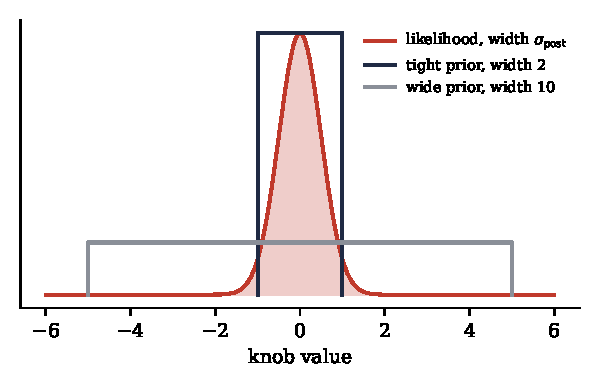
\includegraphics[width=0.85\linewidth]{figures/occam.pdf}
\caption{The Occam factor. The same likelihood (red) under a tight prior and a wide prior. Spreading the prior over a wider range of knob settings lowers its height everywhere, including where the data actually are. A model that ``could have said anything'' is penalised for that freedom automatically.}
\end{figure}

This is Occam's razor with numbers in it. It doesn't say simple models are true. It says a model that could have accommodated a wide range of outcomes gets less credit when the actual outcome turns up, because it spread its bets.

\section{Knobs measured in bits}

There's a neat way to put all knobs on one scale. A knob whose prior range is $\Delta$ and whose data-allowed width is $\sigma$ carries about
\begin{equation}
I=\log_2\frac{\Delta}{\sigma}\ \text{bits}
\end{equation}
of information extracted from the data. That's the number of yes-or-no questions the data had to answer to pin it down. It's also, roughly, minus the base-2 logarithm of the Occam factor.

Take my one galaxy knob, $\kappa$. Suppose before looking you'd have allowed anything from $0.1$ to $10$, a range of 2 dex, and the data pin it to about 5 per cent, or $0.021\dex$. Then
\[
I_\kappa=\log_2\frac{2}{0.0212}\approx6.6\ \text{bits}.
\]
Six and a half yes-or-no questions. Keep that number in mind. We'll compare it with $\log_2(10^{500})\approx1661$ bits in Part~III.

\fig{bits_per_knob}{Information in a knob, $\log_2$ of how much the data shrink its allowed range. Every factor of two is one bit.}


\section{Knobs at the bounds}

One more diagnostic will matter a great deal in Part~II. When you tune a model inside sensible prior ranges and a knob runs to the edge of its range and stays there, the model is telling you something. It wants to go further than its physics allows. A fit with several knobs pinned at their limits isn't a model behaving naturally; it's a model being stretched.

The fried chicken paper reports, for every recipe, how many knobs sit at their bounds. The twelve-knob recipe has three. The ``complete'' recipe of Chapter~7 has seven, against a limit of three set in advance. When half of 171 galaxies push their halo concentration to the same lower edge, that's not scatter. It's a population asking for a different kind of halo.

\section{Freeze first, then turn}

The last knob is the most dangerous because it's invisible: the freedom to decide \emph{after} seeing the results what counts as success. Physicists call this the garden of forking paths, or, less politely, moving the goalposts. The cure is to write the targets down, date them and commit them before the first number is computed. The programme behind this book does this for every calculation, which it calls a \emph{lane}. Each lane commits its criteria to a public repository before any script exists. It also runs a deliberately broken twin, called MUTATE, which must fail; if it passes, the test can't tell right from wrong. Failures are published under the label frozen in advance.

The fried chicken paper's targets were frozen before any recipe was cooked:
\begin{itemize}
\item \textbf{E1}: pooled rms distance to the law at most $0.02\dex$;
\item \textbf{E2}: 95th percentile of per-galaxy rms at most $0.04\dex$;
\item \textbf{E3}: no half-dex bin in $\gbar$ off by more than $0.02\dex$;
\item \textbf{E4}: the fitted scale must vary with the dark energy density as $d\ln a/d\ln\rhoDE=0.50\pm0.05$;
\item \textbf{E5}: the scale's change with redshift must sit inside the law's predicted band.
\end{itemize}
Recipes were added later at my request, and every one of them is disclosed as a dated amendment. The targets never moved.

\section{The rules of knob accounting}

Here are the rules this book will follow, for every theory, including mine.

\begin{enumerate}
\item \textbf{Count every number set by the data being explained.} Global, per-object, hand terms, all of them.
\item \textbf{Count a hand term twice}: once as a knob, and once as a confession that the model didn't produce the behaviour.
\item \textbf{Report knobs at their bounds.} A stretched knob is a model asking for different physics.
\item \textbf{Hold data out.} A fit on unseen data counts for more than a fit on the data used for tuning.
\item \textbf{An imitation proves freedom, not truth.} If a model was tuned to reproduce a target, matching the target tells you the model was flexible enough. It does not tell you the target is real, and it does not tell you the model is right.
\item \textbf{Fewer knobs is a virtue, not a verdict.} A one-knob theory can be wrong, and a hundred-knob theory can be right. Knob-counting tells you how much each theory has risked, and the data decide the rest.
\end{enumerate}

Rule 6 matters most, and it's the one most often broken in popular writing about cosmology, in both directions. Let's go and look at the knobs on the most successful theory in cosmology, and give it the credit it has earned.

\chapter{The Six Knobs That Run the Sky}

\epi{Credit where it's due: six dials, thousands of numbers, one of the best fits in the history of science.\\ Then the fine print.}

\fig[1.0]{plate_cmb_sky}{The sky the six knobs describe. A simulated patch of microwave sky made from a toy power spectrum (not real data): hot and cold spots that differ by about a hundred-thousandth of the average temperature. Underneath, the six dials that set its statistics.}


\section{A universe on six dials}

If you want to see knob economy at its finest, look at the cosmic microwave background. This is the afterglow of the hot early universe, released about 380,000 years after the beginning when the cosmos cooled enough for electrons and protons to combine into neutral hydrogen and let light travel freely. The Planck satellite mapped its temperature and polarisation across the whole sky. Statistically, the map is summarised by power spectra: how much the temperature varies, on average, on each angular scale. The spectra are labelled by multipole $\ell$, where $\ell\approx180^\circ/\theta$ for an angle $\theta$. Planck measured them from $\ell=2$ up to $\ell\approx2500$, in temperature (TT), polarisation (EE) and their cross-correlation (TE). That's thousands of measured numbers.

The spectrum has a shape you can learn to read, like a fingerprint. Each feature is set mainly by one or two of the knobs below, which is why six numbers can pin down thousands of measurements.


\fig{cmb_anatomy}{Reading the microwave spectrum (a cartoon). The large scales carry the primordial seeds; the first peak's position is the acoustic angle; the second peak is lowered by baryons loading the sound waves; the third is driven by dark matter's gravity; and the tail is erased by photons diffusing.}



Base \LCDM\ fits all of them with six knobs. I'll introduce them properly, because in a book about knobs these six deserve a bow before the jokes start.

\section{The expansion: Friedmann's equation}

Everything rests on one equation from general relativity applied to a uniform universe. The expansion rate $H$ at redshift $z$ obeys
\begin{equation}
H^2(z)=H_0^2\left[\Omega_r(1+z)^4+\Omega_m(1+z)^3+\Omega_k(1+z)^2+\Omega_\Lambda\right],
\end{equation}
where $H_0$ is today's expansion rate and each $\Omega$ is a component's share of the critical density $\rho_c=3H_0^2/8\pi G$: radiation (falling as $(1+z)^4$), matter ($(1+z)^3$), spatial curvature ($(1+z)^2$) and the cosmological constant (constant). In base \LCDM\ the universe is flat, $\Omega_k=0$, so $\Omega_\Lambda=1-\Omega_m-\Omega_r$ is not a separate knob. People sometimes say \LCDM\ has seven parameters by counting $\Lambda$ twice. It has six.

\fig{friedmann}{Friedmann's equation, one term at a time. Radiation dominates the early universe, matter takes over at $z\approx3400$, and the cosmological constant takes over only at $z\approx0.3$. The CMB was released in the matter era. (Densities from the standard reading of the expansion history, for illustration.)}


\section{The six, one at a time}

\begin{description}[leftmargin=1em,style=nextline]
\item[1. $\omega_b=\Omega_bh^2\approx0.0224$, the baryon density.] Ordinary matter (protons, neutrons, the stuff of stars and you), with $h=H_0/(100\kms\,\mathrm{Mpc}^{-1})$. Baryons add inertia to the photon fluid. The ratio $R=3\rho_b/4\rho_\gamma$ shifts the balance between gravity and pressure, which makes the compressions (odd-numbered peaks) higher than the rarefactions (even-numbered peaks). The ratio of the first two peaks reads off $\omega_b$ almost directly. It agrees with the deuterium abundance from Big Bang nucleosynthesis, an independent physical process minutes after the beginning. That agreement is one of the great cross-checks in physics.
\item[2. $\omega_c=\Omega_ch^2\approx0.120$, the cold dark matter density.] This is about five times the baryon density. It sets when matter came to outweigh radiation, which controls how strongly the oscillations are driven, and it shapes the third peak, which is sensitive to potential wells that don't oscillate with the photons. It is the amount of a substance that has never been detected in a laboratory.
\item[3. $\theta_*\approx1.041\times10^{-2}$, the acoustic angle.] The sound horizon at last scattering divided by the distance to it:
\begin{equation}
\theta_*=\frac{r_s(z_*)}{D_M(z_*)},\qquad r_s=\int_{z_*}^{\infty}\frac{c_s(z)\,dz}{H(z)},\qquad c_s=\frac{c}{\sqrt{3(1+R)}}.
\end{equation}
It fixes where the peaks fall, and it's measured to about 0.03 per cent, one of the most precise numbers in cosmology. Combined with the others it gives $H_0\approx67.4\kms\,\mathrm{Mpc}^{-1}$.
\item[4. $\tau\approx0.054$, the optical depth to reionisation.] When the first stars and quasars reionised the universe, free electrons re-scattered some CMB light. That suppresses the peaks by a factor of $e^{-2\tau}$ on small scales and creates a bump in polarisation on the largest scales.
\item[5 and 6. $A_s\approx2.1\times10^{-9}$ and $n_s\approx0.965$, the primordial fluctuations.] The initial seeds are assumed to follow a power law,
\begin{equation}
\mathcal{P}_\mathcal{R}(k)=A_s\left(\frac{k}{k_{\rm p}}\right)^{n_s-1},\qquad k_{\rm p}=0.05\,\mathrm{Mpc}^{-1},
\end{equation}
with amplitude $A_s$ and tilt $n_s$. That $n_s$ comes out slightly below 1 is a genuine success for inflation, which predicted a small tilt.
\end{description}

\fig{cmb_cartoon}{What four of the six knobs do to the CMB temperature spectrum. \textbf{This is a cartoon}, a toy oscillation with damping, not a computed spectrum. Baryons raise the odd peaks relative to the even ones; the acoustic angle slides the peaks; reionisation lowers everything above the largest scales; the tilt tips small scales up or down.}


\begin{knobbox}{Base \LCDM\ at the CMB}
Six global knobs: $\omega_b$, $\omega_c$, $\theta_*$, $\tau$, $A_s$, $n_s$. Thousands of measured spectrum values fitted, and the predicted shape of each spectrum carries information on all six at once. By the information measure of Chapter~1, each knob is pinned at the per-cent level or better, which is roughly 6 to 12 bits per knob, on the order of 50 bits for the set. That's an astonishingly good exchange rate.
\end{knobbox}

The acoustic angle deserves a picture of its own, because it is the most precise number in cosmology and it works like a ruler held at arm's length.


\fig{sound_horizon}{The sound horizon as a ruler. Left: a sound wave spreads from every clump in the early universe until the light is released; the distance it has travelled then is $r_s$. Right: seen from across the observable universe, that ruler spans the angle $\theta_*=r_s/D_M$, about 0.6 degrees on the sky.}



\begin{honestbox}[Honesty box: this is the theory's strongest ground]
The CMB is exactly where my own law has nothing to offer. The acceleration scale $a_0$ doesn't appear in the linear equations of a uniform expanding universe, and the programme's record has no CMB fit without a component that behaves, at linear order, like cold dark matter. When the law was run alone on the cosmic web, starting from baryons only, it got the shape of the CMB lensing spectrum wrong under every rule tried (Chapter~12). Any reader who comes away from this book thinking that knob-counting has overturned \LCDM's cosmology has misread it.
\end{honestbox}

\section{The fine print: knobs behind the knobs}

Now the jokes can start. Six is the number on the box. Open it and there are more.

\subsection{Nuisance knobs}

The microwave sky isn't just the CMB. There's dust in our galaxy, radio sources, the cosmic infrared background from distant star-forming galaxies, and the Sunyaev--Zel'dovich effect from hot gas in clusters. Each detector has calibration and beam uncertainties. A real CMB likelihood carries its own nuisance knobs for all of this, of order twenty or more in the high-multipole temperature-and-polarisation likelihood. Most are constrained by priors or by other frequency channels, and they're marginalised over, so they're not freedom in the worrying sense. They are still knobs, and they're the reason ``six parameters'' should always be read as ``six parameters of physical interest.''

\fig{lcdm_panel_full}{The full \LCDM\ control panel. Top: the six. Middle: nine dials left at default settings, any of which can be freed. Bottom: the nuisance dials for foregrounds and calibration. Only the top row is usually quoted.}



\subsection{Hidden knobs: the choices}

The six are six \emph{given} a set of choices: flat geometry, three neutrino species with a minimal mass sum, a helium abundance from nucleosynthesis, a power-law spectrum with no running, no primordial gravitational waves, dark energy as a pure constant. Each of those is a knob fixed at a default value. Freeing them gives the well-known extensions:
\begin{equation}
\{\Omega_k,\ \textstyle\sum m_\nu,\ N_{\rm eff},\ Y_P,\ dn_s/d\ln k,\ r,\ w_0,\ w_a,\ A_{\rm lens},\dots\}
\end{equation}
Each extension is a dial that \LCDM\ can turn if the data demand it. That's legitimate; it's what a framework with a good base model should do. It does mean that the honest count of what the theory \emph{could} accommodate is larger than six. In the language of the Occam factor, the prior is wider than the base model suggests.

One of these deserves a wink. $A_{\rm lens}$ scales the amount of gravitational-lensing smoothing of the CMB peaks. In a consistent theory it must be 1, so it isn't physics but a consistency check. In the 2018 Planck analysis the temperature data preferred a value somewhat above 1. When a knob that is supposed to be fixed at 1 wants to be turned, that's the universe tapping on the glass.

\subsection{The knob with no theory}

$\Omega_\Lambda$ is fixed by flatness, but $\Lambda$ itself is the most embarrassing knob in physics. If it's the energy of the vacuum, a naive quantum estimate with a cutoff at the Planck scale overshoots the measured value by a factor of about $10^{120}$. Even with a much lower cutoff, the mismatch is dozens of orders of magnitude. Nothing in \LCDM\ explains the value; it's simply measured. And it shows up just when it's comparable to the matter density, which is the ``why now?'' coincidence. Keep an eye on this one: my galaxy law ties its acceleration scale to exactly this density, so it inherits the embarrassment rather than curing it.

How big is the embarrassment? It depends where you stop counting the vacuum's energy, but every choice is absurd. Stopping at the scale of the strong nuclear force gives a vacuum energy about $10^{44}$ times too big; stopping at the Planck scale, about $10^{123}$ times.


\fig{vacuum_catastrophe}{The worst estimate in physics. A naive vacuum energy, cut off at four energy scales, against the measured dark energy density. Even the most modest cutoff overshoots by 44 powers of ten.}



\section{Where the six start to creak}

A knob set in one place should give the same value when measured somewhere else. When it doesn't, either the measurement is wrong or the knob is standing in for missing physics. Three such tensions are worth knowing.

\textbf{The Hubble tension.} The CMB, through $\theta_*$ and the model, gives $H_0\approx67$--$68\kms\,\mathrm{Mpc}^{-1}$. The local distance ladder of Cepheids and type Ia supernovae gives about $73$, with errors near one unit. That's a gap of about five standard deviations, persistent for a decade. Either some ladder systematic remains, or one of the default knobs (the early expansion history, perhaps) needs turning.

\fig{h0_tension}{The Hubble tension: the same knob read two ways. The CMB with base \LCDM\ gives about 67.4; the local distance ladder gives about 73.}


\textbf{The clumpiness tension.} Weak lensing surveys tend to find the matter distribution slightly less clumpy (a lower $S_8$) than the CMB-calibrated model predicts. Its significance has varied from survey to survey and has eased in some recent analyses.

\textbf{Dark energy that moves.} In 2024 and 2025 the DESI survey's baryon acoustic oscillation measurements, combined with the CMB and supernovae, preferred dark energy whose density changes with time, parameterised by $w_0>-1$ and $w_a<0$ in
\begin{equation}
w(a)=w_0+w_a(1-a),
\end{equation}
over a pure constant, at roughly 3 to 4 standard deviations depending on the supernova sample. If that holds up, the knob called $\Lambda$ was never a constant, and two more dials ($w_0$, $w_a$) move from ``optional'' to ``required.''

\fig{w0wa_plane}{The dark energy knob plane. The red dot is a cosmological constant, where the law's $a_0$ is exactly constant in time. The shaded quadrant is where recent combined fits have leaned (schematic, no contours drawn). The gold square is the illustrative case worked out in Chapter~13.\label{fig:w0wa}}



That last one matters enormously for this book. In my law the galaxy acceleration scale is tied to the dark energy density, so if dark energy moves, the law says galaxies must notice. We'll come back to this in Part~V. It's the knob that can't be turned.

\section{The scorecard so far}

\begin{center}
\begin{tabular}{lrl}
\toprule
item & knobs & comment\\
\midrule
base physics & 6 & superb fit to thousands of CMB numbers\\
nuisance & $\sim$20+ & mostly prior-constrained; not physics\\
default choices & $\sim$9 & each a dial left at a default\\
$\Lambda$'s value & 1 & measured, unexplained by $10^{120}$\\
dark matter's identity & -- & not a number; a missing particle\\
\bottomrule
\end{tabular}
\end{center}

On the cosmological scale, that's a lean and well-run panel. The trouble starts when you zoom in by a factor of a thousand, from the horizon to a galaxy. There, the six knobs say nothing about what a galaxy should look like, and a whole new panel has to be bolted on. That's next.

\chapter{Where the Knobs Multiply: Galaxies}

\epi{The six knobs build the universe's scaffolding beautifully.\\ Then someone asks what goes on inside a single galaxy,\\ and the panel grows a second floor.}

\section{From the horizon to the halo}

The six knobs of Chapter~2 describe the universe in its smooth, early, linear phase, when every region was within a part in a hundred thousand of average. Galaxies are the opposite: a disc of stars a hundred thousand times denser than average, spinning in a cloud of gas. Between the two lies the nonlinear growth of structure. The six knobs alone can't give you a galaxy; you need to say what happens when gas cools, forms stars, and the stars explode.

\LCDM\ handles this in two layers. The first, dark matter alone, is nearly knob-free. The second, ordinary matter, is where the knobs breed.

\section{Layer one: halos, two numbers each}

Simulate cold dark matter alone, starting from the CMB's initial fluctuations, and it collapses into roughly spherical clumps called halos. In the 1990s Navarro, Frenk and White found that simulated halos share a single profile shape, now called NFW:
\begin{equation}
\rho(r)=\frac{\rho_s}{(r/r_s)\,(1+r/r_s)^2}.
\end{equation}
It falls as $r^{-1}$ near the centre (the ``cusp'') and $r^{-3}$ far out. The enclosed mass is
\begin{equation}
M(<r)=4\pi\rho_sr_s^3\left[\ln(1+x)-\frac{x}{1+x}\right],\qquad x=\frac{r}{r_s}.
\end{equation}
A halo is usually labelled by its mass $M_{200}$, the mass inside the radius $r_{200}$ where the mean density is 200 times critical,
\begin{equation}
M_{200}=\frac{4\pi}{3}\,200\,\rho_c\,r_{200}^3,
\end{equation}
and its \emph{concentration} $c=r_{200}/r_s$. Two numbers per halo, then. Better still, the simulations predict how they're distributed: how many halos of each mass (the mass function) and a mean concentration for each mass, the $c(M)$ relation, with a scatter of about $0.11\dex$. A refinement, the Einasto profile,
\begin{equation}
\rho(r)=\rho_{-2}\exp\left\{-\frac{2}{\alpha}\left[\left(\frac{r}{r_{-2}}\right)^{\alpha}-1\right]\right\},
\end{equation}
adds a third shape number $\alpha\approx0.16$, also predicted rather than tuned.

\fig{nfw_profiles}{Halo shapes. Left: NFW and Einasto densities, with the inner $r^{-1}$ cusp and outer $r^{-3}$ fall-off. Right: circular speed in an NFW halo for three concentrations; more concentrated halos rise faster and peak higher.}


\begin{knobbox}{Layer one: dark matter only}
Per halo: $M_{200}$ and $c$, both drawn from predicted distributions. Shape: NFW or Einasto with $\alpha$ predicted. Global knobs added: essentially none beyond the six. This layer is a genuine prediction of \LCDM\, and it is knob-light.
\end{knobbox}

If galaxies simply sat in these halos, the theory would make sharp predictions. It does, and some of them fail. That is where layer two comes in.

\section{The small-scale headaches}

Over the past thirty years a series of problems have turned up where the dark-matter-only predictions meet real galaxies.

\begin{description}[leftmargin=1em,style=nextline]
\item[Cusp versus core.] Many dwarf and low-surface-brightness galaxies have rotation curves that rise gently, as if the central dark matter density were flat (a core) rather than rising as $r^{-1}$.
\item[Missing satellites.] Simulated Milky Way halos contain hundreds of subhalos massive enough to host dwarf galaxies; far fewer bright satellites are seen. This one is mostly solved by the faintness of small galaxies and the discovery of many ultra-faint ones.
\item[Too big to fail.] The most massive simulated subhalos are too dense at their centres to host the Milky Way's actual bright satellites, yet are too massive to have failed to form stars.
\item[Diversity.] Galaxies with the same maximum rotation speed show a wide range of inner rotation-curve shapes, wider than halos of the same mass predict.
\end{description}

And then there are the regularities, which in some ways are the deeper puzzle.

\section{The regularities: one acceleration scale}

Take a disc galaxy, measure the light from its stars and the radio emission from its gas, and you can compute how fast it \emph{would} spin under Newton's law with no dark matter. Call the resulting gravitational acceleration at radius $r$
\begin{equation}
\gbar(r)=\frac{V_{\rm bar}^2(r)}{r},\qquad V_{\rm bar}^2=V_{\rm gas}|V_{\rm gas}|+\Upsilon_{\rm disk}V_{\rm disk}^2+\Upsilon_{\rm bul}V_{\rm bul}^2,
\end{equation}
where $\Upsilon$ is the stellar mass-to-light ratio, which converts starlight into stellar mass. Measure the actual rotation speed $V$ and you get the observed acceleration $g_{\rm obs}=V^2/r$.

The SPARC sample assembled by Lelli, McGaugh and Schombert in 2016 has 175 disc galaxies with infrared photometry from the Spitzer telescope and good rotation curves. Plot $g_{\rm obs}$ against $\gbar$ for every point in every galaxy, and the points don't scatter all over the place, as you might expect if each galaxy's halo had its own history. They fall on one narrow curve, the \emph{radial acceleration relation}. At high acceleration it follows Newton, $g_{\rm obs}=\gbar$. Below a characteristic scale of about $10^{-10}\ms$ it bends away and follows
\begin{equation}
g_{\rm obs}\approx\sqrt{\gbar\,a_0}.
\end{equation}
At the outer edge of a disc, where the rotation curve is flat at speed $V_f$ and $\gbar\approx GM_b/r^2$, this gives
\begin{equation}
\frac{V_f^4}{r^2}=\frac{GM_b}{r^2}\,a_0\quad\Longrightarrow\quad V_f^4=GM_b\,a_0,
\end{equation}
the \emph{baryonic Tully--Fisher relation}: the fourth power of the rotation speed is proportional to the total mass in stars and gas, with no reference to a halo.

\fig{rotation_anatomy}{Anatomy of a rotation curve, for a toy disc galaxy of $4\times10^{10}M_\odot$ in stars and $10^{10}M_\odot$ in gas. Newton with the visible matter (blue) falls off. The law (red) stays up, heading for $(GM_ba_0)^{1/4}$. A \LCDM\ halo (dashed) can do the same with its two knobs set suitably.}


\fig{rar_toy}{The same toy galaxy in the radial acceleration plane. Under the law its points lie on the red curve by construction. The halo model's points (black) lie close to it too: for one galaxy, a suitably chosen halo can mimic the law. The puzzle is that every galaxy lands on the same curve.}


Mordehai Milgrom predicted both of these in 1983, decades before the data were good enough to check them, as consequences of his modified Newtonian dynamics, MOND. They're among the most striking successful predictions in astrophysics, and \LCDM\ has to explain them as an outcome.

\begin{honestbox}
To be fair to \LCDM: the radial acceleration relation is a relation between two measured quantities, and simulation groups have reported that relations of this kind emerge in their simulated galaxies (for example Ludlow and collaborators, and Keller and Wadsley, both in 2017). A relation emerging isn't the same as the \emph{same} relation emerging, with the same scale, the same shape and the same tightness. That is exactly the question the fried chicken paper asks, and Chapter~8 reports how close the published simulations come.
\end{honestbox}

\section{Layer two: the baryon panel}

To turn a halo into a galaxy, \LCDM\ modelling adds processes that depend on gas physics and star formation. Each one is real physics, and each one comes with knobs.

\subsection{How many stars? Abundance matching}

The first question is how much of a halo's share of baryons becomes stars. The stellar-to-halo mass relation, found by matching the number density of galaxies to the number density of halos, is usually written in the double power-law form of Moster, Naab and White:
\begin{equation}
\frac{M_*}{M_{200}}=2N\left[\left(\frac{M_{200}}{M_1}\right)^{-\beta}+\left(\frac{M_{200}}{M_1}\right)^{\gamma}\right]^{-1}.
\end{equation}
Four knobs: a normalisation $N$, a characteristic mass $M_1$ near $10^{12}\Msun$, a low-mass slope $\beta$ and a high-mass slope $\gamma$. Star formation peaks at a few per cent efficiency near $M_1$ and falls on both sides. In the original paper each of the four also evolves with redshift, which doubles the count.

\fig{shmr}{The stellar-to-halo mass relation and its four knobs. $N$ sets the peak efficiency (a few per cent), $M_1$ its position, $\beta$ and $\gamma$ the slopes either side. Dotted curves show $\beta$ and $\gamma$ turned.}


\subsection{Blowing things up: feedback}

Supernovae and the jets of supermassive black holes heat and expel gas. That suppresses star formation in small and large halos, explaining the shape of the stellar-to-halo relation. Rapid outflows can also shake the dark matter: if gas is repeatedly blown out of the centre and falls back, the gravitational potential fluctuates and dark matter orbits are pumped outward, softening a cusp into a core.

In hydrodynamic simulations these processes happen below the resolution limit, so they're put in as \emph{subgrid} recipes with tunable efficiencies, thresholds and coupling constants. The simulation teams say this openly. The EAGLE project, for example, calibrated its stellar feedback to reproduce the present-day galaxy stellar mass function and galaxy sizes; IllustrisTNG calibrated its model to a set of observed relations. That's a reasonable engineering choice. It also means the calibrated observables are inputs, not predictions.

\subsection{Cores: a recipe}

A popular analytic description of feedback cores is the coreNFW form of Read, Agertz and Collins (2016):
\begin{equation}
M_{\rm cNFW}(<r)=M_{\rm NFW}(<r)\,f^n,\qquad f=\tanh\!\left(\frac{r}{r_c}\right),
\end{equation}
where $r_c$ is a core radius tied to the stellar half-light radius and the exponent $0\le n\le1$ measures how complete the core is. With $n=0$ you have the cusp; with $n=1$ a full core. Two more knobs per galaxy, or two global functions with their own coefficients.

\fig{corenfw}{The coreNFW knob $n$. At $n=0$ the halo keeps its cusp; at $n=1$ the centre is flattened into a core inside $r_c$, and the inner rotation curve rises more slowly.}


\subsection{Squeezing: adiabatic contraction}

Gas cooling into the centre deepens the potential, and the dark matter responds by contracting. The classic model of Blumenthal and collaborators (1986) assumes circular orbits that conserve the adiabatic invariant $rM(r)$:
\begin{equation}
r_i\,M_i(r_i)=r_f\left[M_b(r_f)+(1-f_b)\,M_i(r_i)\right],
\end{equation}
where $M_i$ is the initial total mass profile, $M_b$ the final baryon profile and $f_b$ the baryon fraction. Real halos contract less than this model says, so in practice it's scaled by a contraction fraction, which is another knob, between 0 (none) and 1 (full).

\fig{contraction}{Adiabatic contraction: a $10^{12}M_\odot$ NFW halo before (grey dashed) and after (red) a $5\times10^{10}M_\odot$ disc forms (blue), using the Blumenthal invariant. The dark matter is pulled inward.}


\begin{knobbox}{Layer two: the baryon panel}
\begin{tabular}{@{}lp{6.2cm}@{}}
\toprule
process & typical knobs\\
\midrule
stars per halo & 4 (8 with redshift evolution)\\
feedback energy & efficiency, mass and density scalings\\
core size and strength & 2 per galaxy, or a global function\\
contraction & 1 per galaxy, or a global function\\
halo shape & $\alpha$, $c$ scatter, $M_{200}$ scatter\\
subgrid simulation & dozens of efficiencies and thresholds\\
\bottomrule
\end{tabular}
\smallskip
Every one of these is defensible physics. Every one of them is also a dial.
\end{knobbox}

\section{The question}

So here is the situation. On one side, a regularity in galaxies that looks like it has one acceleration scale, set once for every galaxy, with no visible role for any galaxy's history. On the other side, a theory whose galaxy panel has dozens of dials, each representing real but uncertain physics.

The obvious question is whether the dials can reproduce the regularity. The less obvious and more interesting question is: \emph{how many} dials does it take, \emph{which} ones, \emph{set to what}, and is there anything about the regularity that no dial can reach?

That's an experiment you can actually run. I ran it, and gave it a silly name so nobody would mistake it for a belief. Welcome to the kitchen.


\part{The Fried Chicken Kitchen}
\chapter{The Recipe: Twelve Knobs}

\epi{Preheat the halo to $10^{12}$ solar masses.\\ Season generously with supernovae.\\ Adjust to taste. The taste in question is somebody else's formula.}

\fig[1.0]{plate_recipe_card}{The recipe card. Twelve knobs in four groups, each drawn as a dial. Three of them, in red, ran to the edge of the range I allowed. The card's one honest line: it was tuned to the law, not to the data.}


\section{Why ``fried chicken''?}

The paper this part of the book is built on has a ridiculous title: \emph{ACDM flavored fried chicken version of Galaxy Dynamics}. That is on purpose. It's a research experiment, not a claim. I don't believe the recipes, the halos or the particle readings in it. The point was to work out, carefully and on the record, how a \LCDM\ group \emph{could} reverse-engineer my galaxy law, so that if somebody later presents a tuned match as a derivation, the route is already written down with its knob count attached. ``Fried chicken'' is a nickname with no physics in it. You need a name that nobody will cite as support for anything, and a fast-food name does the job.

The paper went through versions 1.0 to 2.3 between the second and fourth of November 2026, adding a new section every time a new kind of rival recipe was tried. It ran to 48 dated amendments, every one frozen before its numbers were computed, every failed check kept on the record. This chapter and the next four walk through it.

\section{The dish being imitated}

The target is my galaxy law, which Part~IV discusses properly. For now, here it is as a recipe card:
\begin{gather}
\gbar=\frac{g^2}{g+a_0},\\
a_0=\kappa\,c\sqrt{G\rhoDE}=9.36\times10^{-11}\ms,\qquad\kappa=\tfrac12\ \text{(fitted)}.
\end{gather}
Solved for the observed acceleration $g$ given the baryonic one,
\begin{equation}
g_{\rm law}(\gbar)=\frac{\gbar}{2}+\sqrt{\frac{\gbar^2}{4}+\gbar\,a_0}.
\end{equation}
The ingredients are the measured baryons of the SPARC galaxies with fixed mass-to-light ratios, $\Upsilon_{\rm disk}=0.5$ and $\Upsilon_{\rm bul}=0.7$, and no galaxy-by-galaxy adjustment. Four of the 175 galaxies have too few usable points, which leaves 171 galaxies and 3373 points.

\begin{honestbox}
The target is the \emph{law's} curve on each galaxy's own baryons, not the observed rotation curve. This is an imitation contest: can \LCDM's knobs make halos that reproduce the formula? It isn't a contest about which fits the data better. On the observed curves, at these fixed $\Upsilon$, the law's own rms is $0.1951\dex$. Hold onto that number; it comes back with a surprise at the end of the chapter.
\end{honestbox}

\section{How a recipe makes an acceleration}

Every \LCDM\ recipe in the kitchen works the same way. Given a galaxy's baryons, it builds a dark-matter mass profile $M_{\rm DM}(r)$ from its knobs, then adds the halo's pull to the baryons':
\begin{equation}
g_{\rm model}(r)=\gbar(r)+\frac{G\,M_{\rm DM}(r)}{r^2}.
\end{equation}
Compare $g_{\rm model}$ to $g_{\rm law}$ at the same radius, and report three distances (the E1--E3 targets of Chapter~1): pooled rms, the 95th-percentile galaxy, and the worst half-dex bin in $\gbar$.

There's a fourth number, the recipe's own acceleration scale $a$. Fit the law's \emph{form} to the recipe's output, treating $a_0$ as free:
\begin{equation}
a=\arg\min_{a'}\sum_i\Bigl[\log_{10}g_{{\rm model},i}-\log_{10}g_{\rm law}(\gbar{}_{,i};a')\Bigr]^2.
\end{equation}
If the recipe has really learned the law, $a$ should come out at $a_0$.

Before we look at the scores, it helps to see what a distance in dex means on a real rotation curve. Acceleration goes as speed squared, so a gap in acceleration is twice as large, in dex, as the same gap in speed.


\fig{dex_on_curve}{What the scores mean on a rotation curve. The twelve-knob recipe's 0.0415\,dex gap from the law (grey band) is about 5 per cent in speed; the frozen target of 0.02\,dex (red band) is about 2 per cent.}



\section{The menu}

Here is the whole menu, in one table, from the paper's version 2.3. Bold rows pass all three of E1 to E3.

\begin{table}[h]\centering\small
\begin{tabular}{@{}lrrrrr@{}}
\toprule
recipe & knobs & rms & p95 & worst bin & $a/10^{-11}$\\
\midrule
R1 NFW, no tuning & 0 & 0.1419 & 0.2877 & 0.1613 & 15.76\\
R1 tuned, contraction & 4 & 0.0715 & 0.1486 & 0.0441 & 9.12\\
R2 tuned, feedback core & 6 & 0.0721 & 0.1357 & 0.0283 & 8.65\\
R3 thermal, 2 global laws & 2 & 0.2245 & 0.3187 & 0.2261 & 6.06\\
R4 thermal, per galaxy & 342 & 0.0609 & 0.1119 & 0.0260 & 8.97\\
R7 surface density & 9 & 0.0408 & 0.0777 & 0.0413 & 9.21\\
R11 twelve feedback knobs & 12 & 0.0415 & 0.1006 & 0.0221 & 9.33\\
R11b plus $c$ norm, slope & 14 & 0.0275 & 0.0624 & 0.0196 & 9.31\\
R10 six global functions & 42 & 0.0213 & 0.0441 & 0.0216 & 9.30\\
R9 per galaxy, 1$\sigma$ & 1026 & 0.0376 & 0.0711 & 0.0164 & 9.63\\
\textbf{R9 per galaxy, 2$\sigma$} & 1026 & \textbf{0.0152} & \textbf{0.0283} & \textbf{0.0040} & 9.43\\
R8p per galaxy, referee & 684 & 0.0396 & 0.0665 & 0.0148 & 9.72\\
\textbf{R8 per galaxy, wide} & 684 & \textbf{0.0056} & \textbf{0.0130} & \textbf{0.0031} & 9.36\\
\textbf{R6 one empirical function} & 1 & \textbf{0.0075} & \textbf{0.0118} & \textbf{0.0180} & 9.37\\
\textbf{R5 exact shell masses} & 3373 & \textbf{0.0000} & \textbf{0.0000} & \textbf{0.0000} & 9.36\\
\textbf{R12 halo from the formula} & 1 & \textbf{0.0000} & \textbf{0.0000} & \textbf{0.0000} & 9.36\\
\bottomrule
\end{tabular}
\caption{The fried chicken menu: distance to the law in dex. Targets are 0.02, 0.04 and 0.02.}
\end{table}

\begin{figure}[h]
\centering
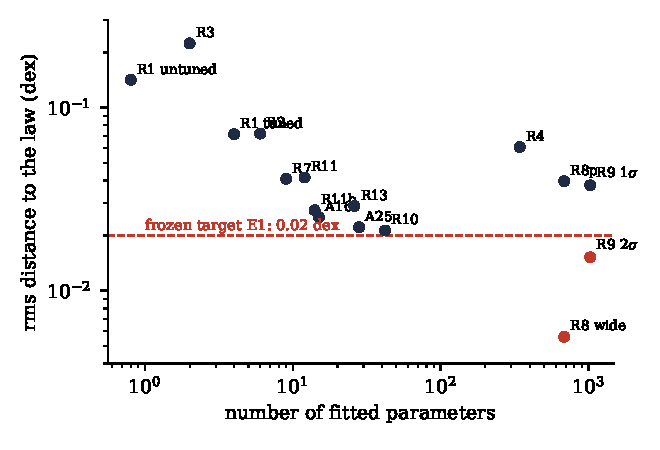
\includegraphics[width=0.92\linewidth]{figures/menu.pdf}
\caption{The knob curve. Each point is a recipe; red points pass the pooled target E1 (dashed). Getting under the line takes either hundreds of per-galaxy knobs or a formula with the law written into it (R5, R6 and R12 aren't plotted; they sit at or near zero by construction).}
\end{figure}

Here is the same menu as a staircase, best recipe at each knob count. Each step down costs more knobs than the last, and the last steps are not recipes at all but the law itself, written as a halo.


\fig{knob_staircase}{Descending the knob staircase. The distance to the law falls as knobs are added, but it crosses the frozen target only with a thousand per-galaxy knobs, or with 3373 knobs that simply restate the law shell by shell.}



We'll come back to the bottom of the menu, where the exact dishes live, in Chapter~5. First, the main course.

\section{Course one: the level comes cheaply}

Start with plain \LCDM: NFW halos, masses from abundance matching, concentrations from the $c(M)$ relation, nothing tuned. That's R1, and it's not close. Its rms distance from the law is $0.1419\dex$, and its acceleration scale is $15.76\times10^{-11}\ms$, about 1.7 times $a_0$. Untouched \LCDM\ halos are too heavy in the middle.

Now turn four knobs: the stellar-to-halo normalisation, the normalisation and mass slope of the concentration relation, and a contraction fraction. The scale drops to $9.12\times10^{-11}$, within 3 per cent of $a_0$.

\begin{honestbox}[The first lesson]
\textbf{Getting the right number from tuned halos is easy, so the number alone proves little.} Four knobs bring \LCDM\ halos to the law's acceleration scale, with the concentration knob sitting at its bound. If you've ever seen ``$\Lambda$CDM reproduces $a_0$'' presented as a deep result, this is the reason for caution. The level is the cheapest part of the law.
\end{honestbox}

Why is the level so cheap? Because in the deep regime the law says $g=\sqrt{\gbar a_0}$, so any model's effective scale is $a=g^2/\gbar$, a single overall amplitude. Anything that moves the overall amount of dark matter in the inner galaxy (halo mass, concentration, contraction) slides $a$ up or down. One knob per direction is enough to hit a target number. The difficult part is the \emph{shape}.

\section{Course two: the shape does not come cheaply}

Halos whose properties depend only on their mass can't follow the law, because the law cares about surface density. Two galaxies with the same mass but different sizes have different $\gbar$ profiles, and the law gives each its own boost. A halo assigned by mass gives them the same.

\fig{level_vs_shape}{Level versus shape. Left: the level knob $a$ slides the law's curve up and down. Right: two discs of the same mass, one compact and one diffuse, in the same halo, compared point by point with the law. The law puts both on one line (red); the shared halo puts them on two different tracks. Fixing that needs knobs that know about surface density.\label{fig:levelshape}}


So the next move is to couple the halo to the galaxy's surface density, $M_b/R_d^2$, where $R_d$ is the disc scale length. Recipe R7 does this with nine knobs and gets to $0.0408\dex$, with the abundance-matching normalisation at its bound. It still misses all three targets.

\section{Course three: twelve knobs of supernova}

The headline recipe, R11, is an analytic stand-in for feedback physics. It's not a hydrodynamic simulation, and the mapping from knob to halo is mine, not any simulation's parameter file. It has twelve global knobs in four groups.

\begin{knobbox}{Recipe R11: twelve supernova knobs}
\textbf{Stellar mass (4).} The Moster stellar-to-halo relation: normalisation, $\log M_1$, $\beta$, $\gamma$.

\textbf{Feedback energy (4).} A dimensionless energy injection
\[
e=\epsilon\left(\frac{M_*}{0.01\,M_{200}}\right)^{a_1}\left(\frac{\Sigma_b}{100}\right)^{a_2}\left(\frac{f_{\rm gas}}{0.5}\right)^{a_4},
\]
with core exponent $n=\tanh e$ in the coreNFW form. Knobs: $\epsilon$, $a_1$, $a_2$, $a_4$.

\textbf{Core size (2).} $\eta=\eta_0\,(M_*/10^9\Msun)^{a_3}$, core radius $r_c=\eta\,R_{1/2}$. Knobs: $\eta_0$, $a_3$.

\textbf{Contraction (2).} Blumenthal fraction $f=f_0+f_1\log_{10}(M_b/10^{9.5}\Msun)$. Knobs: $f_0$, $f_1$.

\medskip
Halos: Einasto with $\alpha=0.16$, concentrations from the Diemer--Joyce $c(M)$ relation.
\end{knobbox}

\fig{recipe_flow}{Recipe R11 as a flowchart, from one galaxy's measured baryons to a grade against the law. Red badges count the knobs at each step: twelve in all.}


Tuned to the law on SPARC, the knobs land at
\begin{center}\small
\begin{tabular}{@{}lrlr@{}}
\toprule
knob & value & knob & value\\
\midrule
$\log N$ shift & $-0.319$ & $\log\epsilon$ & $-0.639$\\
$\log M_1$ shift & $+0.705$ & $a_1$ & $-0.760$\\
$\beta$ shift & $-0.884$ & $a_2$ & $+0.091$\\
$\gamma$ shift & $-0.600$ \ (bound) & $a_4$ & $-0.097$\\
$\log\eta_0$ & $+1.000$ \ (bound) & $a_3$ & $+0.466$\\
$f_0$ & $+1.000$ \ (bound) & $f_1$ & $-0.335$\\
\bottomrule
\end{tabular}
\end{center}
Three of the twelve sit at the bounds of the ranges I chose. Halo masses stay near abundance matching: $\log M_{200}$ shifts by $-0.23$, $+0.11$ and $+0.30$ at the 16th, 50th and 84th percentiles.

\fig{core_exponent}{Two of the tuned knobs at work: the core exponent $n=\tanh e$ as the feedback energy changes with star-formation efficiency, at three surface densities. The tuned slope $a_1=-0.76$ gives the biggest cores to the least efficient galaxies.}


The result:
\begin{itemize}
\item the recipe's acceleration scale is $a=9.331\times10^{-11}\ms$, \textbf{within 0.3 per cent of $a_0$};
\item its rms distance from the law is $\mathbf{0.0415\dex}$, a typical gap of about 10 per cent;
\item tuned on half the galaxies, it scores $0.0405$ there and $0.0445$ on the half it never saw, so it transfers.
\end{itemize}
It doesn't pass E1, which needs $0.02$. But it's close.

\fig{train_test}{Do the recipes generalise? Each was tuned on one set of galaxies (blue) and graded on galaxies it had never seen (red). Most hold up: the patterns the knobs found are real patterns. The widened 28-ingredient recipe (A25) is the exception, the sign of a recipe fitting noise.}



Add two more knobs, a normalisation and slope for the $c(M)$ relation, and you have R11b with fourteen knobs. That reaches $0.0275\dex$ ($0.0326$ on unseen galaxies), with halo masses raised by a median $0.39\dex$ and both new concentration knobs at their bounds.

\section{The plot twist: the observed curves}

None of these recipes was tuned to observed rotation curves; they were tuned to my formula. So it's fair to ask how they do on the real data, at the same fixed $\Upsilon$. Here's the answer, in rms dex against the observed curves of the same 171 galaxies:

\begin{center}
\begin{tabular}{lrr}
\toprule
model & knobs & rms to observed curves\\
\midrule
the law & 1 & 0.1951\\
R7 surface density & 9 & 0.1964\\
R11 twelve knobs & 12 & 0.1953\\
R11b fourteen knobs & 14 & 0.1933\\
\bottomrule
\end{tabular}
\end{center}

They're indistinguishable. The fourteen-knob recipe is very slightly \emph{better} than the law on this statistic.

\fig{observed_tie}{The plot twist. Against the observed rotation curves, at fixed mass-to-light ratios, the law and the tuned recipes are indistinguishable: all four sit within 0.003\,dex.}


\begin{honestbox}[The second lesson]
With these fixed mass-to-light ratios, a good fit to rotation curves alone can't pick the law over a tuned halo. The scatter in this statistic is dominated by the observational errors and the fixed-$\Upsilon$ assumption, not by the difference between the models. So anybody who says ``the law fits rotation curves better than \LCDM'' on the basis of this kind of comparison is overclaiming, and that includes me if I ever say it. What the law has is not a better fit. It's the same fit with one knob instead of twelve, and the twelve were tuned \emph{to the law}.
\end{honestbox}

\fig{needle_haystack}{Why rotation curves alone can't decide. The residuals against observed curves spread by about 0.195\,dex for every model; the difference between the law and a tuned recipe is 0.003\,dex. The two curves are drawn on top of each other, and you can't see the gap.}



\section{A side dish that didn't work: the thermal halo}

One idea deserves a mention because it looked like the natural imitator and isn't. If dark matter particles interact enough to thermalise in a galaxy's centre, the inner halo becomes isothermal, with a profile set by the baryons' potential. Kaplinghat, Tulin and Yu argued in 2016 that this can produce the diversity of rotation curves. Recipe R3 tries it with two global laws and fails badly: $0.2245\dex$. Even with 342 per-galaxy parameters (R4) it gets only to $0.0609$.

There's a curious footnote. The per-galaxy fits land near a relation between the isothermal dispersion $\sigma$ and the baryon mass,
\begin{equation}
\sigma^4\approx\frac{G\,M_b\,a_0}{4},
\end{equation}
with a median ratio of 1.017. That's the baryonic Tully--Fisher relation in disguise, $V_f^4=GM_ba_0$ with $V_f=\sqrt2\,\sigma$, the textbook relation between circular speed and dispersion for an isothermal sphere. The halo has been tuned to carry the law, and it shows. But the scatter is wide, ratios from 0.568 to 3.174, so it's no more than a tendency.

\section{What the twelve knobs taught us}

\begin{enumerate}
\item The \textbf{level} of the law, its acceleration scale, comes almost for free. Four knobs get within 3 per cent; twelve within 0.3 per cent.
\item The \textbf{shape} costs more. Twelve knobs reach $0.0415\dex$, fourteen reach $0.0275$, and neither passes the frozen $0.02$ target.
\item On the \textbf{observed} curves the tuned recipes and the law are indistinguishable at fixed $\Upsilon$. Fit quality alone doesn't decide.
\item The recipes needed \textbf{knobs at their bounds} to get there: three of twelve, both new knobs of fourteen.
\end{enumerate}

So far the knobs have done well. In the next chapter we let them do whatever they like, and then we add up the bill.

\chapter{The Exact Dish, and Its Bill}

\epi{Anything is on the menu if you don't look at the prices.}

\fig[0.8]{plate_bill}{The bill for the exact dish, itemised. Each line is a number from this chapter. The subtotal is a perfect match; the last line is the one item no \LCDM\ kitchen stocks.}


\section{Ordering everything}

Chapter~4 played fair: a handful of global knobs, one recipe for every galaxy. This chapter takes the gloves off. What if every galaxy gets its own knobs? What if we write down the halo the law would need and simply call it a halo? What if the recipe is the formula with a new name?

Each of these gets closer to the law. Each passes or nearly passes the frozen targets. And each comes with a bill that says, in the plainest possible terms, where the match came from.

\section{R9: six knobs per galaxy, inside the priors}

Recipe R9 is the closest match to the law using only \LCDM\ parts within stated priors. Each galaxy gets its own
\begin{equation}
\{\,M_{200},\ c,\ \alpha_{\rm Einasto},\ f_{\rm contraction},\ n_{\rm core},\ r_c\,\},
\end{equation}
six knobs times 171 galaxies, 1026 in all. Each knob may move only within a set range around its \LCDM\ expectation: abundance matching for $M_{200}$, the $c(M)$ relation for $c$, with fixed ranges for the shape, contraction and core knobs.

With ranges of one standard deviation of each relation (0.11\,dex in $c$, 0.3\,dex in $M_{200}$) R9 fails, at $0.0376\dex$. Widen to 2$\sigma$ (0.22\,dex in $c$, 0.6\,dex in $M_{200}$) and it passes all three targets: rms $0.0152$, 95th percentile $0.0283$, worst bin $0.0040$.

\begin{knobbox}{R9's bill}
\begin{itemize}
\item 1026 knobs. BIC rent at $n=3373$: about 8335.
\item Median $\log c$ shift: $-0.22$, \textbf{at the bound}.
\item Median Einasto $\alpha$: 0.1, \textbf{also at the bound}.
\end{itemize}
Scatter can't push half of all galaxies to the same edge of a prior. When the median galaxy wants its concentration at the limit, the priors aren't describing scatter around \LCDM's halos; they're describing a population shift away from them. R9 is really saying ``give me halos about 40 per cent less concentrated than \LCDM\ predicts, for everybody.''
\end{knobbox}

\section{R8: let it all hang out}

Remove the priors almost entirely and you get R8: each galaxy gets its own $M_{200}$, $c$, contraction fraction and core exponent, 684 knobs, using NFW, Blumenthal contraction and a coreNFW core. It nails the law: rms $0.0056\dex$, about 1.3 per cent.

The bill, relative to abundance matching and the $c(M)$ relation: $\log M_{200}$ shifts by a median $+0.29$ and by $+1.2$ at the 84th percentile, more than ten times heavier than abundance matching allows. $\log c$ shifts by a median $-0.42$, reaching $-0.81$ at the 16th percentile, so halos six times less concentrated than predicted. Contraction is near full (median 0.9). Put the priors back at the referee's values, 0.11\,dex in $c$ and 0.3\,dex in $M_{200}$, and the same recipe (R8p) is $0.0396\dex$ and fails.

\fig{bill}{The bill, in pictures: how far each exact or near-exact dish pushes halos from \LCDM's relations. Shaded bands are 1$\sigma$ and 2$\sigma$ prior widths. Concentrations go low across the board; halo masses go high, except in the biggest galaxies, where the law wants halos several times lighter than abundance matching.}


\section{R10: the knobs as functions}

Per-galaxy knobs are the polynomial-through-the-points of Chapter~1. A fairer test of whether there's a \emph{recipe} hiding in them is to write the six per-galaxy knobs as smooth functions of each galaxy's measurable properties. R10 makes each of the six a quadratic in baryon mass, surface density and gas fraction: 42 coefficients, one recipe for everybody.

It stops just short: $0.0213\dex$, and $0.0270$ on unseen galaxies. But look at the halos it builds. The median $\log M_{200}$ shift is $+0.46$ and the median $\log c$ shift is $-0.74$. \textbf{Zero of 171 galaxies} lie inside 1$\sigma$ of both \LCDM\ relations. It's a recipe, but not for \LCDM\ halos.

\section{R6: the one-knob halo}

Now go the other way. There's a published one-line formula for the radial acceleration relation, from McGaugh, Lelli and Schombert (2016):
\begin{equation}
g_{\rm obs}=\frac{\gbar}{1-\exp\!\left(-\sqrt{\gbar/g_\dagger}\right)}.
\end{equation}
Read it as a halo: whatever $g_{\rm obs}-\gbar$ is, that's the dark matter. With one knob, $g_\dagger=9.585\times10^{-11}\ms=1.024\,a_0$, recipe R6 passes E1 to E3 at $0.0075\dex$.

One knob, a pass. Isn't that as good as my law? Not as a \LCDM\ recipe, because nothing in \LCDM\ produces it. It writes the law's content as a halo response with no process behind it. It's modified dynamics in a trench coat, standing on a dark matter halo's shoulders.

\section{R5: the law, renamed}

Finally, the logical end point. Define the dark matter at each measured radius as whatever is needed to make the law come out:
\begin{equation}
M_{\rm DM}(r)=\frac{r^2}{G}\Bigl[g_{\rm law}(\gbar(r))-\gbar(r)\Bigr].
\end{equation}
Do this shell by shell, and you have 3373 knobs for 3373 points. The rms is $0.0000\dex$. It's the polynomial through all the points.

\fig{shells_knobs}{Recipe R5, drawn. Every shell of every galaxy gets its own dial for the dark mass inside it, set to whatever makes the law come out. That's one knob per data point: 3373 knobs for 3373 points.}



\fig{needed_halo}{The halo the law needs, for the toy galaxy of Chapter~3, defined shell by shell as $M_{\rm DM}=r^2(g_{\rm law}-g_{\rm bar})/G$, beside an ordinary NFW halo. For one Milky-Way-like galaxy the two look alike, which is why the level is cheap. The bill comes from fitting all 171 galaxies at once.}


That sounds like a joke, but it raises a serious question. \emph{Could} such a halo exist? A mass profile isn't automatically a physical halo; it has to be made of particles on real orbits with positive probabilities. That's checkable.

\begin{mathbox}{Can a halo be made of particles? Eddington's test}
For a spherical, isotropic, collisionless system, the phase-space distribution function depends only on energy, $f=f(\mathcal{E})$, where $\mathcal{E}=\Psi-\tfrac12v^2$ is the binding energy and $\Psi=-\Phi$ the relative potential. Eddington showed in 1916 that the density determines $f$ uniquely:
\[
f(\mathcal{E})=\frac{1}{\sqrt8\,\pi^2}\,\frac{d}{d\mathcal{E}}\int_0^{\mathcal{E}}\frac{d\rho}{d\Psi}\,\frac{d\Psi}{\sqrt{\mathcal{E}-\Psi}}.
\]
A halo is physically possible as such a system only if $f(\mathcal{E})\ge0$ for every $\mathcal{E}$. Two weaker checks come first: the density must be positive, and the isotropic Jeans equation,
\[
\frac{d(\rho\sigma^2)}{dr}=-\rho\,\frac{d\Phi}{dr},
\]
must give a positive velocity dispersion $\sigma^2$ everywhere.
\end{mathbox}

\fig{eddington}{Eddington's test can fail. Left: a Hernquist sphere has a positive distribution function at every energy, so it can be built from particles. Right: a cored tracer around a point mass needs negative numbers of stars at some energies, so it can't. R5's halos pass this test in 171 of 171 galaxies.}

The Jeans check is easier to picture. Treat the needed halo as a cloud of particles moving in the galaxy's total gravity, and ask how fast they must move, on average, to hold the cloud up. If the answer were negative anywhere, no such cloud could exist.


\fig{jeans_check}{The Jeans check, on the toy galaxy of Chapter~3. The velocity spread the halo's particles need (green) is positive everywhere, between about 90 and 150\,km\,s$^{-1}$, so a halo of particles can hold this shape. For the 171 real galaxies the paper finds the same.}




The paper ran all three checks on R5's halos, with the baryons smoothed by $0.1\dex$. Density positive: 171 of 171. Isotropic Jeans dispersion positive: 171 of 171. Eddington distribution function non-negative (to 1 per cent of its peak): 171 of 171. To make sure the code could actually fail, it was run on two known cases: it returns $+0.0000$ for a Hernquist sphere, which is physical, and $-0.2555$ for a cored tracer in a point-mass potential, which famously isn't.

\begin{honestbox}[The third lesson]
\textbf{Stability is no argument against the imitation.} A halo made of particles, in equilibrium, can reproduce the law exactly in every SPARC galaxy, at least within the measured radii. ``Dark matter can't do that'' is false as a statement about equilibria. What dark matter has trouble with is \emph{getting there}, which is the next section.
\end{honestbox}

\section{Where would R5's halos come from?}

A halo that exists in equilibrium today must have formed somehow. In \LCDM\ it formed as an NFW-like halo and was then modified by baryons. So run the clock backward: undo the adiabatic contraction and ask what the halo looked like before the galaxy formed.

Undoing Blumenthal contraction gives a monotonic initial profile in 158 of 171 galaxies; in the other 13 it isn't. An NFW fit to the initial profiles has a median rms of $0.057\dex$ and $0.261\dex$ at the 84th percentile, so some are nothing like NFW. The median fitted concentration is \textbf{0.32 of the $c(M)$ value}, a third as concentrated as \LCDM\ predicts. The implied halo mass has median shift $+0.16\dex$ from abundance matching, but $-0.76$ at $\log M_b$ 11 to 12: the biggest galaxies want halos six times lighter than abundance matching gives them.

So the exact halo exists but is hard to grow. That's the origin problem, and no knob fixes it.

\section{R12: the halo defined from the formula}

At my request the paper added one more dish, frozen as Amendment A6: a single function for every galaxy that \emph{is} the law, including its tie to dark energy.
\begin{gather}
M_{\rm DM}(r)=\frac{r^2}{G}\Bigl[g_{\rm law}(\gbar;a)-\gbar\Bigr],\\
a=\kappa\,c\sqrt{G\rhoDE},\qquad\kappa=\tfrac12\ \text{by hand}.
\end{gather}
In \LCDM's language this is a halo of collisionless particles with the particle unspecified. Only the mass profile enters, so it says nothing about the particle's mass or identity. R5's Eddington check is what licenses that reading.

It passes everything by construction:
\begin{itemize}
\item rms distance to the law: $0.0000\dex$;
\item rms to the observed curves: $0.1951$, identical to the law;
\item $\kappa=0.500$ in all three test cosmologies;
\item slope with the dark energy density: $+0.500$;
\item $a(z)/a(0)=1.000$ for constant dark energy, inside the law's band.
\end{itemize}
\textbf{None of that is evidence.} The formula went in, so the formula comes out.

\begin{knobbox}{R12's bill}
\begin{enumerate}
\item \textbf{A coupling \LCDM\ doesn't have.} A particle halo has no term through which it could know the dark energy density. The tie needs a new interaction that isn't one of \LCDM's knobs. It's not a knob setting; it's new physics.
\item \textbf{No formation path.} R5's origin problem stands.
\item \textbf{Halo masses off at the top.} The implied $\log M_{200}$ sits a median $+0.11\dex$ from abundance matching (16th to 84th percentile $-0.23$ to $+0.27$), but $-0.80$ at $\log M_b$ 11 to 13.
\end{enumerate}
One item is \emph{not} on the bill: baryon fractions. $M_b/M_{200}$ stays below the cosmic value of 0.156 in all 171 galaxies, so the exact halo doesn't run out of dark matter.
\end{knobbox}

\section{The menu, re-read}

Line the dishes up by what they cost:

\begin{center}\small
\begin{tabular}{@{}lrl@{}}
\toprule
dish & knobs & what the match is made of\\
\midrule
R11 & 12 & real \LCDM\ processes, tuned to the law; close, not exact\\
R11b & 14 & the same plus stretched concentrations; closer\\
R10 & 42 & smooth functions; halos outside \LCDM\ for all 171\\
R9 & 1026 & per-galaxy, inside 2$\sigma$; a population shift in $c$\\
R8 & 684 & per-galaxy, no priors; halos up to 10$\times$ off\\
R6 & 1 & the empirical relation, renamed a halo\\
R5 & 3373 & the law, shell by shell\\
R12 & 1 & the law plus its tie, written as a halo\\
\bottomrule
\end{tabular}
\end{center}

The pattern is a seesaw. Recipes that stay close to \LCDM's predicted halos miss the law. Recipes that hit the law do so either with hundreds of per-galaxy knobs pushed to their limits, or by containing the law. There's no point on the menu that is both a natural \LCDM\ halo and an exact match.

And every one of them, apart from R12, which got the tie by having it typed in, has the same hole. None of them knows about dark energy. That's the ingredient no knob supplies, and it's the subject of the next chapter.

\chapter{The Ingredient No Knob Supplies}

\epi{You can tune a halo to taste.\\ You cannot tune it to know what the vacuum weighs.}

\section{What ``tied to dark energy'' means}

My law doesn't just say galaxies have an acceleration scale of about $10^{-10}\ms$. It says what that scale \emph{is}:
\begin{equation}
a_0=\kappa\,c\sqrt{G\rhoDE},
\end{equation}
where $\rhoDE$ is the density of dark energy, the same quantity that drives the accelerating expansion of the universe. With $\kappa=\tfrac12$ and the dark energy density implied by today's expansion, $\rhoDE\approx5.84\times10^{-27}\,\mathrm{kg\,m^{-3}}$ (about 3.3\,GeV per cubic metre, a few protons' worth), this gives $a_0=9.36\times10^{-11}\ms$.

The idea of tying Milgrom's scale to the dark energy density isn't mine. Limbach, Psaltis and \"Ozel proposed it in 2008, and Milgrom pointed out the numerical nearness of $a_0$ to $cH_0$ and to $c^2\sqrt\Lambda$ in his first papers. What this programme adds is a reconstruction of how that scale should change over time and a graded record of whether anything else can produce it.

The tie has three operational consequences, and each is a test any imitation has to pass.
\begin{enumerate}
\item \textbf{The slope.} In a universe with a different dark energy density, $a_0$ must change as $\rhoDE^{1/2}$:
\begin{equation}
\frac{d\ln a_0}{d\ln\rhoDE}=\frac12.
\end{equation}
\item \textbf{The constant.} The coefficient $\kappa$ must come out the same in every cosmology. It's a property of the law, not of our particular universe.
\item \textbf{The history.} As the universe ages, $a_0$ must follow the dark energy density, not the matter density or the expansion rate:
\begin{equation}
\frac{a_0(z)}{a_0(0)}=\sqrt{\frac{\rhoDE(z)}{\rhoDE(0)}}.
\end{equation}
If dark energy is a cosmological constant, $a_0$ is the same at every redshift.
\end{enumerate}
These are the fried chicken paper's targets E4 and E5, frozen before anything was cooked. To test them, each recipe is put into other universes: three cosmologies with different $(\Omega_\Lambda,H_0)$, holding the physical matter densities and fluctuation amplitude fixed, and the same universe at redshifts 1, 1.5 and 2.33.

\section{What the knobs do in other universes}

Take R10, the 42-coefficient recipe from Chapter~5, with no help. In other universes its scale moves the wrong way:
\begin{itemize}
\item slope with $\rhoDE$: $+0.283$, against $0.50$;
\item effective $\kappa$: 0.459, 0.614 and 0.735 across the three cosmologies, against a constant;
\item $a(z)/a(0)$: 1.58, 2.12 and 3.44 at $z=1$, 1.5 and 2.33, against a band near 1.
\end{itemize}

The redshift drift is the instructive part, because it follows from simple halo physics.

\begin{mathbox}{Why halo accelerations rise with redshift}
A halo of mass $M_{200}$ has, by definition, mean density $200\rho_c(z)$ with $\rho_c=3H^2/8\pi G$. So
\begin{gather*}
M_{200}=100\,\frac{H^2r_{200}^3}{G}\quad\Longrightarrow\\
V_{200}^2=\frac{GM_{200}}{r_{200}}=100\,H^2r_{200}^2,\qquad V_{200}=10\,H\,r_{200}.
\end{gather*}
A characteristic acceleration of the halo is then
\[
a_{\rm halo}\sim\frac{V_{200}^2}{r_{200}}=10\,H\,V_{200}\ \propto\ (GM_{200})^{1/3}H^{4/3},
\]
using $V_{200}=(10\,GM_{200}H)^{1/3}$. At fixed mass and concentration, a halo's acceleration scale grows as $H^{4/3}$. By $z=2.33$ the expansion rate is about 3.5 times today's, so a halo of the same mass and concentration has an acceleration scale about $3.5^{4/3}\approx5.3$ times larger. Concentrations evolve and galaxies grow, which softens that, but the direction is set: halo scales follow the expansion rate and the matter density. Nothing in this pulls toward the dark energy density.
\end{mathbox}

\fig{halo_vs_z}{How each scale changes with redshift. The law with a cosmological constant is flat. The rival $a\propto H$ and the untuned recipe climb; a halo at fixed mass and concentration climbs fastest, as $H^{4/3}$. Only the recipe with hand terms typed in stays near flat.}


\section{Hand terms: typing the tie in}

To make R10 pass, the paper wrote dependences in by hand, five terms in all. With
\begin{equation}
c\propto\rhoDE^{\,3.00}\,H_0^{-1.61},\qquad M_{200}\propto H_0^{-12},
\end{equation}
the slope becomes $+0.496$, which passes, and $\kappa$ reads 0.485, 0.506 and 0.525 across the cosmologies, a narrow miss of the 5 per cent target. And with
\begin{equation}
c\propto(1+z)^{-0.26-0.89z}
\end{equation}
the redshift ratios become 0.93, 0.91 and 0.92, inside the band.

\begin{knobbox}{Counting those hand terms}
Five hand terms, two at the bounds the paper allowed. Each must be counted twice under the rules of Chapter~1: once as a knob, and once as a confession. Concentration rising as the dark energy density \emph{cubed}? Halo mass falling as the twelfth power of the Hubble constant? No process produces these. And the redshift term only works with the baryons held fixed in time, which no real galaxy does. When you have to type the tie in, it's the law's physics written into the halo.
\end{knobbox}

\section{Does \texorpdfstring{\LCDM}{LCDM} contain the tie already?}

A rival would reasonably say: never mind knobs, there are acceleration scales in \LCDM\ that involve $\Lambda$. Maybe one of them is the tie. Amendment A13 asked exactly that, with five gates frozen first: $\kappa_{\rm eff}$ within $0.05\dex$ of $\tfrac12$; slope $0.50\pm0.05$ across cosmologies; inside the redshift band; one constant over halo masses $10^{10}$ to $10^{15}\Msun$; and acting on galaxy dynamics. Here are the candidates.

\subsection{Milgrom's coincidence}

The cosmological constant has its own acceleration. In a de Sitter universe two test particles separate as $\ddot r=(\Lambda c^2/3)\,r$, and the natural scale is
\begin{equation}
a_\Lambda=\frac{c^2}{2\pi}\sqrt{\frac{\Lambda}{3}}.
\end{equation}
Using $\Lambda c^2=8\pi G\rhoDE$, this is
\begin{equation}
a_\Lambda=\frac{c}{2\pi}\sqrt{\frac{8\pi G\rhoDE}{3}}=\underbrace{\frac{1}{2\pi}\sqrt{\frac{8\pi}{3}}}_{0.461}\;c\sqrt{G\rhoDE}.
\end{equation}
So $\kappa_{\rm eff}=0.461$, slope exactly $+0.500$, and flat in redshift if dark energy is constant. It passes three gates out of the box.

It fails the fifth. The cosmological constant's actual pull on a star 10\,kpc from a galaxy's centre is
\begin{equation}
g_\Lambda=\frac{\Lambda c^2}{3}\,r=\frac{8\pi G\rhoDE}{3}\,r\approx1.0\times10^{-15}\ms\approx1.1\times10^{-5}\,a_0.
\end{equation}
It acts on nothing in a galaxy. A rival can quote $\Lambda$ for the \emph{value}, but no \LCDM\ process carries it into halos. That outcome was written down before the run.

\fig{lambda_pull}{The cosmological constant's push against a galaxy's pull. At 10\,kpc $\Lambda$ pushes with a hundred-thousandth of $a_0$; it only reaches $a_0$ about a gigaparsec out. Its \emph{scale} is near $a_0$; its \emph{force} in a galaxy is negligible.}


\subsection{The expansion rate}

$cH_0/2\pi$ gives $\kappa_{\rm eff}\approx0.551$ on the dark energy footing, but if galaxies knew about $H$ rather than $\rhoDE$, the scale would rise 3.432 times by $z=2.33$. That's the rival law $a_0\propto H(z)$ of Part~V, and it fails E5.

\subsection{The NFW central acceleration}

There's a natural acceleration inside every NFW halo, $2\pi G\rho_sr_s$. At $M_{200}=10^{12}\Msun$ it's $0.830\,a_0$, intriguingly close. But over halo masses it spans $-0.46$ to $+0.48\dex$, and it scales with cosmology at slopes of $+1.381$ and $+3.561$ (against 0.5).

\subsection{The baryonic Tully--Fisher scale}

Feed the cosmic baryon fraction into $V^4/GM_b$ and you get $0.202\,a_0$, spread over $0.505\dex$. No.

\begin{mathbox}{The $c$-barrier: why halo scales near $a_0$ are a coincidence}
The tie contains the speed of light: $a_0=\kappa c\sqrt{G\rhoDE}$. Writing $\rhoDE=\Omega_\Lambda\cdot3H_0^2/8\pi G$,
\[
a_0=\kappa\sqrt{\frac{3\Omega_\Lambda}{8\pi}}\;cH_0\approx0.143\,cH_0\quad(\kappa=\tfrac12,\ \Omega_\Lambda=0.685).
\]
A halo's acceleration, built from $G$, $M_{200}$ and $H$, has no $c$ in it:
\[
a_{\rm halo}=10\,H\,V_{200}\times F(c_{\rm NFW}),
\]
where $F$ depends only on concentration. For $2\pi G\rho_sr_s$, $F=c_{\rm NFW}^2/2m(c_{\rm NFW})$ with $m(x)=\ln(1+x)-x/(1+x)$. So
\[
\frac{a_{\rm halo}}{a_0}=\frac{10\,F(c_{\rm NFW})}{0.143}\cdot\frac{V_{200}}{c}.
\]
For $M_{200}=10^{12}\Msun$, $V_{200}\approx143\kms$ and $c/V_{200}\approx2102$. The factor $10F/0.143$ must therefore be about 2000 to land near $a_0$, and it is: for $c_{\rm NFW}=8$, $F\approx33.6$ and $a_{\rm halo}\approx0.81\,a_0$. A factor of two thousand from the overdensity convention and the concentration happens to cancel a factor of two thousand in $c/V_{200}$. Change the mass and $V_{200}$ changes as $M^{1/3}$; change the cosmology and nothing in $F$ knows. The nearness is a coincidence at one mass, not a tie.
\end{mathbox}

\fig{c_barrier}{The $c$-barrier. A halo's central acceleration relative to $a_0$ across halo masses, with an illustrative $c(M)$ relation (Dutton and Macci\`o 2014). It crosses $a_0$ near $10^{12}M_\odot$ and misses by a factor of 2 to 3 at the ends. The top axis shows the factor of about two thousand, $c/V_{200}$, that the overdensity and concentration factors happen to cancel near that mass.}


Amendment A35 graded every place where $\rhoDE$ enters \LCDM\ structure formation and found no tie; the native collapse-epoch route gives $\kappa_{\rm eff}=0.4358$, and it isn't a tie either.

\section{The strongest swoop}

The best rival move came in Amendment A15, and in the spirit of the book I'll give it its due. It's the argument of Navarro and collaborators (2017): over the mass range of disc-galaxy hosts, $\log M_{200}$ from 11 to 12.5, the NFW central acceleration varies by only $0.089\dex$. So maybe the law's scale is just the typical halo's inner acceleration.

Per SPARC galaxy, through the stellar-to-halo relation, that acceleration has a median of $0.612\,a_0$ and a spread of $0.156\dex$, with $\kappa_{\rm eff}=0.306$, and it rises 1.493 times by $z=2.33$. On its own it doesn't supply the tie. But multiply it by \textbf{one global factor, 1.404}, use each galaxy's own halo scale in the law's formula, and it sits $0.0586\dex$ from the law and $0.1941\dex$ from the observed curves, against the law's $0.1951$.

\begin{honestbox}[What the strongest swoop shows]
One knob on \LCDM\ halos ties the law on today's rotation curves. What it lacks is the tie to dark energy and a flat $a_0(z)$. And here's the uncomfortable part, in the paper's own words: on observable gates alone, since one universe has one $\rhoDE$, Milgrom's coincidence can't be told from the tie. Only a mechanism separates them, or a measurement of how the scale changes with time. That's why Part~V exists.
\end{honestbox}

\section{Coincidences are cheap}

How easy is it to find a number near $a_0$ by combining \LCDM's constants? Amendment A27 counted. It built 199,584 acceleration expressions from the constants of \LCDM\ ($G$, $c$, $H_0$, the density parameters, the baryon fraction and so on) and asked how many pass the number, slope and redshift gates. 104 do, 63 of them distinct values. With the target deliberately slid off its true value, the expected number of chance hits is 62.1.

So 63 distinct hits against 62.1 by chance: \emph{exactly what you'd expect from numerology}.

\fig{coincidences}{Numerology, counted. Of 199,584 acceleration formulas built from \LCDM's constants, the number that pass all three gates is what chance alone predicts.}
 Most of them are the $\Lambda$ coincidence dressed up with other ratios. None reaches galaxy radii. The lesson cuts against everyone, including me. A formula that lands near $a_0$ isn't special on that basis alone. The programme ran this test on my own formula too, in a lane called CG1. The test lacks the power to call any formula special at today's precision, and it gives my formula no statistical support for being special either. That doesn't refute it; it just means the formula has to earn its keep through predictions, not through numerical nearness.

\section{Plus one ingredient}

Amendment A14 tried \LCDM\ plus one named extra ingredient. Feedback as encoded in the stellar-to-halo relation gives $1.715\,a_0$ at $10^{12}\Msun$ but spreads $0.830\dex$ over mass and rises 3.2 times by $z=2.33$. A halo edge set by $\Lambda$, at the radius where the halo's pull equals $\Lambda$'s push, is flat in redshift but only $0.001\,a_0$, and it grows as $M^{1/3}$. Coupled quintessence rescales $G$ for dark matter and carries no acceleration scale. A product of halo gravity and $\Lambda$'s pull gives $0.005\,a_0$.

Then the paper turned to the one route that \emph{does} put $\rhoDE$ into halos: interacting vacuum, where dark energy exchanges energy with dark matter at a rate $Q=\xi H\rho$ (Amendment A20). Near $\xi=-0.35$ it gives $\kappa_{\rm eff}$ between 0.456 and 0.550. But the halo scale drifts with redshift, spreads $0.152\dex$ between galaxies, and put into the law's formula it sits $0.0577\dex$ away.

\section{The scorecard for the tie}

\fig{tie_gates}{The tie's gates, route by route. Each row is a way a rival could try to get $a_0=\kappa c\sqrt{G\rho_{\rm DE}}$; each column is a frozen gate. Only R12, which has the law typed in and needs a coupling \LCDM\ lacks, passes them all.}


\begin{center}\small
\begin{tabular}{@{}lll@{}}
\toprule
route & what it gets & what it misses\\
\midrule
knobs, no hand terms & slope $+0.283$ & $\kappa$ runs; rises $3.44\times$\\
knobs plus 5 hand terms & slope $+0.496$, band & terms no process makes\\
$\Lambda$ coincidence & $\kappa$ 0.461, slope, flat & acts on nothing ($10^{-5}a_0$)\\
$cH/2\pi$ & $\kappa$ 0.551 & rises $3.43\times$\\
NFW centre & $0.830\,a_0$ at $10^{12}$ & $\pm0.5\dex$ over mass\\
strongest swoop & law on today's curves & no tie, rises $1.49\times$\\
interacting vacuum & $\kappa$ 0.46--0.55 & drifts in $z$, spreads\\
199,584 formulas & 63 hits & 62.1 expected by chance\\
\bottomrule
\end{tabular}
\end{center}

Every route gets one or two pieces. None gets the law and the tie together. The only dish that has both is R12, and R12 has them because they were typed in, with a coupling to dark energy that \LCDM\ doesn't contain.

That's the central finding of the fried chicken experiment, so here it is in one line: \textbf{knobs can make the law, but they can't make it know about dark energy.}

\chapter{The High Priest's Complete Recipe}

\epi{Twenty-six knobs walk into a cluster.\\ Seven of them are pinned to the wall.}

\section{Beyond rotation curves}

So far the kitchen has cooked for one customer, the SPARC rotation curves. A real theory has to feed everyone: gravitational lensing around galaxies, the hot gas in galaxy clusters, the dark energy tie and the Solar System. The paper's next move, at my request, was to ask for the complete meal. Build one global \LCDM\ recipe, using the law as its basis, that passes every line on a scoreboard frozen in advance. I called it the high priest's recipe, because it's the one a determined defender of the faith would cook.

First, though, the new customers.

\section{Lensing: the bending of light around galaxies}

A galaxy's mass bends the light of galaxies behind it, slightly distorting their shapes. Averaging the distortion over many foreground galaxies (lenses) gives the excess surface density profile, $\Delta\Sigma(R)$, the mean surface density inside projected radius $R$ minus that at $R$:
\begin{equation}
\Delta\Sigma(R)=\bar\Sigma(<R)-\Sigma(R),\qquad\Sigma(R)=\int\rho\!\left(\sqrt{R^2+z^2}\right)dz.
\end{equation}
The KiDS-1000 survey measured this for isolated lens galaxies (Brouwer and collaborators, 2021) in four bins of stellar mass, 60 points from 35\,kpc out to 2.6\,Mpc, with a full covariance matrix. Lensing reaches far beyond the visible discs, which makes it a strong test of what the halo does where rotation curves can't see.

The recipes need extra knobs to face lensing. Out at a megaparsec, a lens's signal includes its neighbours, through a two-halo term with a large-scale bias $b(M)$ from Tinker and collaborators (2010):
\begin{equation}
\Delta\Sigma=\Delta\Sigma_{\rm 1h}+b(M)\,\Delta\Sigma_{\rm lin}.
\end{equation}
The plain law has neither a truncation nor a two-halo term; it is applied as is. All models were graded against the gate $p\ge0.01$ with nothing refitted, frozen before the numbers in Amendments A4 to A6.

\begin{table}[h]\centering\small
\begin{tabular}{@{}lrrr@{}}
\toprule
model & $\chi^2$, 60 pts & $\chi^2$, $R\le1$\,Mpc (44) & amplitude $A$\\
\midrule
plain law, R12 untruncated & 276.1 & 211.4 & 1.367\\
R12 cut at $R_{200}$, two-halo & 457.7 & 290.4 & 1.422\\
R11 twelve knobs & 277.9 & 146.5 & 1.179\\
R11b fourteen knobs & 242.1 & 120.9 & 1.140\\
base \LCDM\ control, untuned & 563.1 & 444.2 & 0.809\\
\bottomrule
\end{tabular}
\caption{KiDS-1000 isolated lenses. Every row fails the $p\ge0.01$ gate. $A$ is one fitted scale factor, a diagnostic only; 1 means no offset.}
\end{table}

\begin{honestbox}
Every model fails, mine included. The recipes, tuned only to the law on SPARC, don't lose to the law here; the fourteen-knob recipe does better. A halo made more realistic by a cutoff does worse. A post-result diagnostic with a free mass shift in each bin (so not a grade) gives the law 167.7 on 56 degrees of freedom at $+0.2$ to $+0.3\dex$, close to an earlier independent run of 163.1 on the same file. All the rows may share a problem with lens masses or the covariance. In Chapter~12 we'll see that the law has a real lensing shortfall of about $0.09\dex$ inside 0.3\,Mpc that survives every estimator the programme has.
\end{honestbox}

\fig{kids_chi2}{The lensing grade on KiDS-1000. Every single-recipe model fails the $p=0.01$ line. Only R14's patchwork of about 1066 parameters gets under it (on 46 degrees of freedom, line 71.2).}


\section{Clusters: the X-COP test}

Galaxy clusters are the other big customer. X-COP is a sample of clusters with excellent X-ray data, where the hot gas's temperature and density profiles give the total mass through hydrostatic equilibrium:
\begin{equation}
M_{\rm HSE}(<r)=-\frac{k_BT(r)\,r}{G\mu m_p}\left[\frac{d\ln n_e}{d\ln r}+\frac{d\ln T}{d\ln r}\right].
\end{equation}
Clusters are where modified dynamics has always struggled, and my law is no exception. On X-COP the law's mean log offset is $-0.467\dex$ with rms $0.476$. In mass terms, the hydrostatic mass is 2.93 times what the law provides from the visible baryons, and all seven clusters come up short (Chapter~12). \LCDM\ halos, by contrast, are at home here.

\section{R13: the high priest's recipe}

R13 is one global recipe tuned jointly to the law on SPARC, to KiDS lensing and to X-COP hydrostatic masses, frozen as Amendment A10. Its ingredients:

\begin{knobbox}{R13: 21 knobs plus 5 hand terms}
\begin{itemize}
\item R11b's 14 feedback and concentration knobs;
\item an AGN core cutoff for massive systems;
\item a lens mass offset;
\item a two-halo multiplier;
\item a satellite fraction and host mass;
\item a hydrostatic bias;
\item a cluster baryon fraction;
\item and the 5 dark-energy and redshift hand terms from Chapter~6.
\end{itemize}
It was tuned on half of each dataset and graded on the rest, then tuned on everything.
\end{knobbox}

The first run had an X-COP radius error of a factor of 1000 and two smaller errors. They were fixed under the same gates and the wrong output was kept on the record. Here's the frozen scoreboard.

\begin{table}[h]\centering\small
\begin{tabular}{@{}p{4.3cm}p{2.6cm}l@{}}
\toprule
line & R13 & result\\
\midrule
L1 distance to the law (0.02, 0.04, 0.02) & 0.0290, 0.0640, 0.0187 & fail (E3 passes)\\
L2 rms to observed SPARC ($\le0.205$) & 0.1943 & pass\\
L3 KiDS, 60 points, $p\ge0.01$ & $\chi^2=145.2$ & fail\\
L4 X-COP mean, rms (0.05, 0.12) & $-0.001$, 0.075 & pass\\
L5 slope with $\rhoDE$; $\kappa$ & $+0.500$; 0.483, 0.49, 0.51 & pass\\
L6 $a(z)/a(0)$ & 0.929, 0.913, 0.92 & pass\\
L7 Cassini, smooth halo & $2.0\times10^{-9}\,a_0$ & pass\\
L8 unseen SPARC, KiDS, X-COP & 0.0281; 82.1 on 30; 0.048 & fail on KiDS\\
L9 knobs at bounds ($\le3$); $M_{200}$ shift ($\le0.3$) & 7; 0.32 & fail\\
\bottomrule
\end{tabular}
\caption{R13's frozen scoreboard. Verdict: \textbf{not complete}.}
\end{table}

Four fails out of nine. And two of the passes are softer than they look.

\fig{r13_scoreboard}{R13's frozen scoreboard as tiles. Light green marks passes that rest on hand terms or a parameter at its bound.}


\textbf{The dark energy passes are typed in.} L5 and L6 pass because of the hand terms, which are still extreme: $c\propto\rhoDE^{3.00}H_0^{-4.86}$ and $M_{200}\propto H_0^{-9.54}$. Without them the slope is $+0.245$.

\textbf{The cluster pass is propped up.} L4 passes with the cluster baryon fraction at its lower bound of 0.08, when the sample's measured value in one system is 0.138, and with the hydrostatic bias at zero. That's a poor physical reading, so the X-COP pass is weak.

\section{R14: escalation}

When R13 failed, the obvious next move was to give the recipe more freedom, and the paper did, frozen as Amendment A11. R14 uses R9's 1026 per-galaxy parameters on SPARC, and adds 14 per-bin parameters for lensing on R13's halo.

It gets lensing to pass: $\chi^2=69.6$ on 60 points, $p=0.014$ at 46 degrees of freedom, and 44.7 on 28 unseen radii, $p=0.024$. Four of the 14 new knobs are at their bounds, including truncation at three times $R_{200}$ and the host mass.

Count it up: 1026 per galaxy, 14 per lensing bin, R13's 21 knobs and 5 hand terms. About \textbf{1066 parameters}. And it's a patchwork. Nothing connects R9's per-galaxy values to the lensing side, and the hand terms weren't rechecked on R9's halos. It's not one theory; it's a quilt.

\section{The honest reading}

This is the chapter where it would be easy to crow, so let me be precise about what was found.

\textbf{Getting close is easy.} A dozen knobs get the law's level, nearly its shape, and a tie with the law on observed rotation curves.

\textbf{Getting everything at once, as one theory, wasn't achieved here.} R13, with 26 knobs and hand terms, fails four of nine lines. R14 passes more lines with about 1066 parameters, but it isn't a single theory.

\textbf{And on two datasets, the tuned recipe beats the law.} On X-COP the law's mean offset is $-0.467$ with rms 0.476; R13 gets $-0.001$ with rms 0.075. On KiDS the law's $\chi^2$ is 276.1 against R13's 145.2. The tuned \LCDM\ recipe fits clusters and lensing better than my law. It does so with a weak physical reading in clusters and hand terms for the tie, but it does.

\fig{xcop_compare}{X-COP clusters: the law comes up short by about half a dex; the tuned recipe lands on the data, with a baryon fraction at its lower bound.}


\textbf{Not graded:} the CMB and growth on the recipe, cluster keys, dwarfs, IC~1613, the Milky Way, the Bullet Cluster, wide binaries and any formation path.

\begin{honestbox}[The fourth lesson]
A complete \LCDM\ recipe that contains the law and its tie wasn't found. That doesn't refute \LCDM: real hydrodynamic simulations could do things a semi-analytic model can't, and \LCDM\ never claimed to contain my law. What the experiment does show is that if a \LCDM\ paper ever claims to \emph{derive} this law, it has five things to show: the per-galaxy priors on $M_{200}$ and $c$; the fit against surface-density diversity, not just mass; the slope with $\rhoDE$ with baryons evolved; $\kappa$ across cosmologies; and a formation path to the required halos. Passing those would be a real result, and the law would then have to be read as an output of the halo side.
\end{honestbox}

\section{An interlude: what if the halo were a particle?}

Since R5 and R12 showed that equilibrium halos can carry the law, the paper took the reasoning one step further, in the rival's language. I don't hold this reading. The point is to see what a reverse-engineered particle would need.

\textbf{A field version.} A static scalar field with
\begin{equation}
\frac{y^2}{a_0-y}=\gbar
\end{equation}
reproduces the law to $3.9\times10^{-13}$ on all 3373 points in spherical symmetry, so $y<a_0$ everywhere. It's not new: it's the scalar function $\mu_s=\tilde\mu/(1-\tilde\mu)$ of Zhao and Famaey (2006) for the simple interpolating function of Famaey and Binney (2005).

\textbf{A particle version.} If a real particle halo supplies all of $g_{\rm law}-\gbar$, there's no extra force on baryons, so no double counting. Such a halo can't bind to the Sun beyond 0.076\,AU, so the Solar System passes, and wide binary stars should be Newtonian, unlike a field reading of the law.

\textbf{Its bill.} A boson that condenses in all of SPARC but not in clusters at 100\,kpc lands between 9.2 and 13.7\,eV. But the pressure at fixed density scatters by $0.521\dex$ between galaxies against a limit of 0.1, so no single equation of state holds these halos up. The halos need a median of 0.516 of \emph{all} the supernova energy available, at full coupling. Tracking baryons by scattering would need $\sigma/m$ of 0.63 to 40\,cm$^2$\,g$^{-1}$. A fermion needs a mass above about 56\,eV for a typical galaxy and 245\,eV for the most demanding. And nothing in any of it puts the dark energy density in the halo.

\textbf{A posited action.} Amendment A12 wrote the link as one action with one scale:
\begin{gather}
L=-\rhoDE\left[1+\frac{\kappa^2}{4\pi}H(s)\right]-\frac{\kappa}{\sqrt{8\pi}}\frac{\phi\,\rho_b}{M_{\rm Pl}},\\
s=\frac{|\nabla\phi|}{\sqrt{\rhoDE}},\qquad H'(s)=\frac{s^2}{1-s}.
\end{gather}
It gives $a_0=\kappa c\sqrt{G\rhoDE}$ and reproduces the law to $0.00004\dex$, with the field's gradient energy capped at $\rhoDE$. It's a posit, not a derivation. $\kappa$ stays fitted, the free function leaves the vacuum constant free and turns complex for timelike gradients, so the action has no cosmology yet. Close neighbours exist in the literature: Banik and Zhao's observation that a gravitational field's energy density reaches the dark energy density at $c^2\sqrt\Lambda$, and a Skordis--Z\l{}o\'snik extension that ties the MOND scale to the dark energy potential.

The particle detour ends where every road in this kitchen ends. Everything can be imitated. The dark energy tie has to be put in by hand.

\chapter{Every Other Kitchen in Town}

\epi{A restaurant guide to the dark sector.\\ Stars awarded for flavour. Nobody gets the fourth star.}

\section{The crawl}

Once the main recipe was on record, the obvious objection was: you only tried \emph{your} version of \LCDM. What about self-interacting dark matter? Fuzzy dark matter? The simulations themselves? Superfluids, dipoles, emergent gravity? So, over a single long day, the paper went on a restaurant crawl. Amendments A16 through A48 each took one more kitchen and graded it on the same frozen gates: the distance to the law (rms $\le0.02$, 95th-percentile galaxy $\le0.04$, worst bin $\le0.02$, unseen galaxies $\le0.025$), and whether the scale ties to $\rhoDE$, including, from A29 on, a tracking gate where dark energy evolves.

Here's the guide. Ratings are mine and carry no physics; the numbers are the paper's.

\section{More knobs on the same stove}

\textbf{A16, the knob blocks.} Four new blocks of knobs added to the fourteen-knob recipe, keeping whatever helps. The best set has 15 knobs and reaches $0.0263\dex$; with widened bounds $0.0252$, at a median halo mass $0.64\dex$ (4.4 times) above the stellar-to-halo relation. On unseen galaxies it gives $0.0267$, and the per-galaxy 95th percentile, $0.053$, blocks it. This is the closest single recipe in the whole paper.

\textbf{A25, the kitchen sink.} 28 \LCDM\ ingredients stacked into one global recipe: the 14 feedback knobs, the A16 blocks, two published halo-response forms, a self-interacting core, adiabatic contraction, separate settings for gas-rich and bulge galaxies, the slope and scatter of the stellar-to-halo relation. Plot distance against knob count and the curve \emph{flattens}, near $0.022\dex$; 28 knobs give $0.0222$. Widen the bounds and it reaches $0.0204$, but $0.0370$ on unseen galaxies, at a plausibility cost of 1.29 range-widths outside the literature. Its $\kappa_{\rm eff}$ of 0.497 is inherited from the target, and its scale still rises about three times by $z=2.33$.

\begin{knobbox}{The plateau}
Adding knobs stops helping at about $0.022\dex$. That's the most interesting single number in this chapter. A model that could reach the law if only it had enough freedom would keep descending as knobs are added. A plateau means the remaining gap is a shape the ingredients can't make, not a level they can't reach.
\end{knobbox}

\textbf{A26, the same recipe in other universes.} The frozen 14-knob recipe, put into universes with different $\rhoDE$, moves with slope $+0.187$ to $+1.453$ depending on what's held fixed, against 0.5. By $z=2.33$ its scale is 3.02 to 4.55 times today's. You'll see that bar again in the figure of Chapter~13.

\section{Other kinds of dark matter}

\begin{description}[leftmargin=1em,style=nextline]
\item[Wave (fuzzy) dark matter, A17.] A solitonic core on an NFW halo, from an ultralight boson. The boson mass alone gives $0.149\dex$; six knobs give $0.092$. The fits improve by \emph{switching the soliton off}: at six knobs it survives in none of the 171 galaxies, and the soliton's acceleration scale grows with halo mass.
\item[Hydro-calibrated halo responses, A18.] Published formulas fitted to simulations (Di Cintio and collaborators 2014, coreNFW, and the FIRE-2 form of Lazar and collaborators 2020) sit $0.116$ to $0.177\dex$ from the law; with three knobs each, $0.073$ to $0.084$, wanting lighter halos.
\item[Self-interacting dark matter, A19 and A41.] Velocity-dependent cross-section: $0.122\dex$, $0.080$ with three halo knobs. Per-galaxy halo masses and concentrations at $\sigma/m=0.5$\,cm$^2$\,g$^{-1}$, in the style of Ren and collaborators (2019): $0.0487$ with 343 parameters, 77 at a bound, and $0.110$ on unseen galaxies. On its collapsed branch, $0.179$; with each galaxy free to choose its branch, $0.047$ with 514 parameters but $0.110$ unseen.
\item[Warm and mixed dark matter, A19 and A41.] $0.116$ to $0.120$.
\item[Condensate dark matter, A41.] A fixed core radius gives $0.129$, with no core solution at all in 83 of 171 galaxies.
\item[Decaying dark matter, primordial black holes, dark radiation, a Yukawa force, A42.] Best $0.0717$, with every fitted particle parameter beyond published limits. The black holes, for example, come out at $4\times10^5\Msun$, which would also overheat the discs.
\item[Dark mass that traces the gas, A43.] $0.41$ as published, $0.21$ with a stellar term, because bright discs hold too little gas.
\item[Halo flattening, tides, substructure, environment, A44.] Moves the best 28-knob recipe from $0.0222$ to $0.0221$. The plateau doesn't budge.
\end{description}

\section{The simulations themselves}

The fairest test of all would be real hydrodynamic simulations, which the paper can't run. Amendment A21 used their published results instead, as read from the papers. No measured simulation scale reaches the law. The closest is Magneticum, $0.0290\dex$, then MassiveBlack-II's faint galaxies at $0.0306$ and ZOMG at $0.0359$; EAGLE's raw fits sit $0.17$ to $0.19\dex$ away. Only round, order-of-magnitude figures of ``$10^{-10}\ms$'' pass. The EAGLE runs with varied $\Lambda$ report no acceleration relation, so the slope with $\rhoDE$ can't be tested from any simulation on record. Where redshift numbers exist, the scale rises into the past, by 1.305 to 1.428 times in ZOMG.

\begin{honestbox}
These simulation values come from the papers' summaries and are provisional. Simulations are the one kitchen this book can't fully inspect, and a future simulation could do better than anything graded here. If one does, and passes the five tests of Chapter~7, that would be a real result.
\end{honestbox}

\section{The near-MOND kitchens}

Several theories reproduce modified-dynamics phenomenology from something else. They're interesting because they're closest in spirit to my law.

\textbf{Superfluid dark matter, A22} (Berezhiani and Khoury, 2015). Dark matter condenses in galaxies into a superfluid whose phonons mediate an extra force on baryons. Its deep force, $\gbar+\sqrt{a\gbar}$, sits $0.0392\dex$ from the law. Setting its energy scale by $\Lambda^4=\rhoDE$ gives $\kappa_{\rm eff}=5.01$, ten times too big; reaching 0.5 needs its coupling set by hand, so $\kappa$ just moves into the coupling.

\textbf{Dipolar dark matter, A23} (Blanchet and Le Tiec, 2008). Its published cubic function gives the same $\gbar+\sqrt{a\gbar}$ and the same $0.0392$. Its free function \emph{can} take the law's shape exactly: a fourth-order expansion with three knobs reaches $0.0036$. But that's a fit of shape inside a reformulation of MOND, not a \LCDM\ mechanism, and its link to $\Lambda$ is stated as an order of magnitude and imposed.

\textbf{Emergent gravity, A24} (Verlinde, 2017). Best $0.0392$ with one knob. With today's $H_0$ it gives $\kappa_{\rm eff}=0.583$ and rises 3.51 times by $z=2.33$. With the de Sitter rate $\sqrt{\Lambda/3}$ it gives $\kappa_{\rm eff}=0.482$, slope 0.5 and no drift, but its effective scale spreads $0.115\dex$ between galaxies, and the choice of rate is imposed. It's the $\Lambda$ coincidence of Chapter~6 with $1/6$ in place of $1/2\pi$.

\begin{mathbox}{Three theories, one wrong shape}
Superfluid, dipolar and emergent gravity all reduce, in their plain forms, to
\[
g_{\rm sum}=\gbar+\sqrt{a\,\gbar},
\]
while the law is
\[
g_{\rm law}=\frac{\gbar}{2}+\sqrt{\frac{\gbar^2}{4}+a\,\gbar}.
\]
Both go to $\sqrt{a\gbar}$ in the deep regime ($\gbar\ll a$), and both go to $\gbar$ in the Newtonian regime, but at different rates. The excess over Newton is $g-\gbar\to\sqrt{a\gbar}$ for the sum, which keeps growing, and $g-\gbar\to a$ for the law, which saturates. At the transition, $\gbar=a$:
\[
g_{\rm sum}=2a,\qquad g_{\rm law}=\tfrac12a+\sqrt{\tfrac54}\,a=1.618\,a,
\]
the golden ratio, as it happens. The gap there is $\log_{10}(2/1.618)=0.092\dex$. Averaged over SPARC's points, it's the $0.0392\dex$ that all three theories share. Same functional form, same miss: the transition has the wrong shape.
\end{mathbox}

\fig{sum_vs_law}{Three theories, one shape. Left: the boost $g/g_{\rm bar}$ for the law and for the sum form $g_{\rm bar}+\sqrt{ag_{\rm bar}}$. Right: their difference, which peaks near the transition, where the law gives the golden ratio and the sum form gives 2.}


\section{Fitting the observed curves directly}

Amendment A28 changed the question. Forget imitating the law; fit each galaxy's \emph{observed} rotation curve with mass-to-light ratio, distance and inclination free within published priors, and compare cored \LCDM\ halos with my law (with its dark energy tie).

\textbf{Here the rival wins.} Cored halos fit better than the tied law even after paying the BIC rent: total BIC 17804.6 against 19744.2, and they beat the law in 154 of 171 galaxies.

But the fitted galaxies, put back through the radial acceleration relation, give a relation $+0.056$ to $+0.103\dex$ off the tied $a_0$, with $0.125$ to $0.137\dex$ of scatter. So they reproduce the data \emph{without} reproducing the law. A better fit is not a derivation, and it isn't proof for either side. The paper's verdict: \textbf{the swoop that works is fitting the curves galaxy by galaxy; the one that fails is deriving the law and its tie.}

\section{Evolving dark energy and the rival literature}

Amendments A29 to A40 added the sharpest gate: where dark energy evolves, the scale must follow $\sqrt{\rhoDE(z)}$ to within $0.05\dex$ at $z=1$, 1.5 and 2.33.

\textbf{\LCDM\ halos follow the wrong thing.} In evolving backgrounds, halo scales follow the expansion rate and the matter density, not dark energy. Their slope with $\rhoDE$ runs from $-0.124$ to $+0.026$, and none of 315 $w_0$--$w_a$ backgrounds passes with the 14-knob recipe frozen (A29). Tuning feedback and dark energy together reaches tracking only through fitted powers of $H(z)$ with no named process, $H^{+3.0}$ on the stellar-to-halo relation and $H^{+4.2}$ on feedback (A32), which then distort the curves at high redshift and fail on unseen galaxies.

\textbf{The best rival line in the literature (A34).} The cooling scale of Kaplinghat and Turner (2002), one of the earliest \LCDM\ explanations of a MOND-like scale, put inside the law's formula and multiplied by one factor, 0.398, set by hand, matches today's curves exactly: $0.0152\dex$, $0.0156$ unseen. The shape is borrowed from the law, and the scale is tuned. It follows the matter density, not $\rhoDE$, and rises 1.42 times by $z=2.33$. Disc-formation and halo-response papers miss by 0.12 to $0.22\dex$.

\textbf{Screened fields (A30).} A three-knob k-mouflage fit with no halo reaches the law's shape, $0.0086\dex$, because its switch lies below almost every point and it acts as a power law. It adds $61.6\,a_0$ at Saturn, which the Cassini spacecraft would have noticed, and its scale doesn't depend on $\rhoDE$. Chameleon, symmetron and coupled quintessence fail.

\textbf{The logotropic fluid (A36)} of Chavanis carries the slope 0.5 natively, the only route that does without help, but its halo pull caps at $0.298\,a_0$ where the law needs $0.618\,a_0$, and its scale stays flat as dark energy evolves.

\textbf{De Sitter and quantised inertia (A37)} share one shape, $0.0189\dex$ with a free constant, but fail the worst bin at $0.0273$, with $\kappa_{\rm eff}=0.651$. Dark matter tied to baryons (A38): $0.072$ at best. Clustering dark energy (A39): at most $0.1\,a_0$ in halos. Correlated halo scatter (A40): best $0.154$.

\section{Modified gravity and systematics}

The last four amendments asked whether other modified-gravity theories, or plain measurement error, could produce the law with its tie.

\textbf{Modified gravity (A45, A46).} Vainshtein-screened DGP and Galileon gravity leave galaxies Newtonian, $0.496\dex$ from the law (or $0.142$ with a \LCDM\ halo). Beyond-Horndeski theories have no acceleration scale. In relativistic MOND theories (TeVeS, AeST, bimetric MOND) $a_0$ is a constant written into the Lagrangian, and where the interpolation is free it can be chosen to be the law, which is a choice, not a derivation. TeVeS's standard function is the sum form, $0.10$ at its usual $a_0$. MOG misses by $0.377$, conformal gravity by $0.136$.

\textbf{Measurement systematics (A47, A48).} Is the law just what ordinary halos look like through imperfect measurements? Non-circular motions, bars, pressure support, disc thickness, beam smearing, selection, mass-to-light trends and gas uncertainties, applied to \LCDM\ mocks at literature amplitudes, reach at best $0.122\dex$. Every mock keeps an excess of $+0.13$ to $+0.16\dex$ in the lowest-acceleration bin. A selection weight towards weak halos reaches the scale, $\kappa_{\rm eff}=0.518$, but not the shape.

\begin{honestbox}[A systematic that cuts my way, and against me]
The same corrections, applied to the \emph{real} SPARC data, raise the law's own fitted $a_0$ by up to $+0.101\dex$. Allowed mass-to-light and gas changes move it by $-0.174$ to $+0.157\dex$. In other words, my one knob, $\kappa=\tfrac12$, carries a systematic uncertainty of order $\pm0.15\dex$, roughly 30 to 40 per cent either way. That's a big reason why $\kappa$ is described as fitted and why the data can't single out $\tfrac12$ (Chapter~10).
\end{honestbox}

\section{The guide, summarised}

\fig{kitchens_map}{Every kitchen on one map: best distance to the law against number of knobs. \LCDM\ recipes (dark) flatten out near 0.022\,dex. The kitchens that get below the target (green) do it by putting the law's shape in by choice. None ties the scale to dark energy.}


\begin{table}[h]\centering\small
\begin{tabular}{@{}lrrl@{}}
\toprule
kitchen & knobs & best dex & tie to $\rhoDE$?\\
\midrule
\LCDM\ feedback, A16 & 15 & 0.0252 & no\\
kitchen sink, A25 & 28 & 0.0222 & inherited; rises $3\times$\\
Kaplinghat--Turner, A34 & 1 + law shape & 0.0152 & no; rises $1.42\times$\\
simulations, A21 & (published) & 0.0290 & untestable\\
superfluid, A22 & 1 & 0.0392 & $\kappa$ 5.0 natively\\
dipolar, A23 & 3 & 0.0036 & imposed\\
emergent, A24 & 1 & 0.0392 & imposed rate\\
k-mouflage, A30 & 3 & 0.0086 & no; fails Saturn\\
logotropic, A36 & native & caps at $0.3\,a_0$ & slope yes; flat in $z$\\
SIDM per galaxy, A19 & 343 & 0.0487 & no\\
coreNFW on data, A28 & per galaxy & beats law on BIC & law not reproduced\\
\bottomrule
\end{tabular}
\caption{Every other kitchen. None gets the law \emph{and} the tie natively.}
\end{table}

Nobody gets the fourth star. Some kitchens reach the law's shape (dipolar, k-mouflage) by choosing a free function. Some reach today's curves exactly by borrowing the law's form and tuning a scale (Kaplinghat--Turner). One beats the law outright on observed curves (per-galaxy cored halos) without reproducing the law. And not one of them, on its own terms, makes the acceleration scale follow the density of dark energy.

Which brings us to a theory with rather more freedom than any kitchen in town.


\part{A Knob With \texorpdfstring{$10^{500}$}{10\textasciicircum 500} Clicks}
\chapter{The Landscape: A Knob With \texorpdfstring{$10^{500}$}{10\textasciicircum 500} Clicks}

\epi{Zero knobs on the front panel.\\ A warehouse out back with $10^{500}$ of them, and no map.}

\fig[1.0]{plate_landscape}{The landscape, drawn. Every valley is a possible vacuum, a universe with its own constants of nature. String theory's equations allow an astronomical number of them, and nothing yet says which valley is ours.}


\section{A theory with no knobs at all}

After eight chapters of counting knobs in \LCDM's kitchen, you might expect string theory to be the opposite case, and in one sense it is. Its admirers point out, rightly, that string theory has \emph{no} adjustable dimensionless parameters in its fundamental formulation. There's a string length, which sets the units, and that's it. The coupling strength isn't a knob; it's the value of a field. Every number in physics, in principle, is supposed to come out of the theory.

That's an extraordinary ambition, and it's worth pausing to admire it. The Standard Model of particle physics has around nineteen free parameters, and more once you include neutrino masses: particle masses, mixing angles and coupling strengths, all measured and none explained. \LCDM\ adds its six. A theory that derived all of them from nothing but geometry would be the greatest achievement in the history of science.

The catch is in the phrase ``in principle.''

\section{Where the knobs went}

Superstring theory is consistent in ten spacetime dimensions. We see four. The other six must be curled up, \emph{compactified}, into a tiny space, and the physics we see in four dimensions depends on the shape and size of that space. The favoured candidates are Calabi--Yau manifolds, six-dimensional spaces with special properties that preserve some supersymmetry.

\fig{garden_hose}{How a dimension can hide. Up close, a garden hose is a two-dimensional surface; from far away it looks like a one-dimensional line. String theory curls up six extra dimensions this way, far too small to see.}



How many Calabi--Yau shapes are there? Nobody knows if the number is finite. One classical construction, as hypersurfaces in toric varieties, uses four-dimensional reflexive polytopes; Kreuzer and Skarke enumerated those in 2000 and found 473,800,776. Each gives at least one Calabi--Yau space, and many give more.

\fig{counts_ladder}{How big the numbers are, measured by how many digits it takes to write them: about nine for the count of four-dimensional reflexive polytopes, 500 for the famous estimate of flux vacua, and 272,000 for one F-theory geometry.}



Each shape also comes with continuous deformations, called \emph{moduli}: sizes and shape parameters that can vary smoothly without changing the topology. Their counts are given by the Hodge numbers $h^{1,1}$ and $h^{2,1}$. The quintic threefold, the simplest textbook example, has $h^{2,1}=101$ complex-structure moduli. In four dimensions every modulus shows up as a massless scalar field, which would mediate a long-range force that experiments don't see. So the moduli have to be fixed, or \emph{stabilised}.

That's where the knobs come from. The theory doesn't have them in its equations. It has them in its \emph{solutions}.

\section{Fluxes: how to build a discretuum}

The standard way to stabilise moduli is with fluxes: generalised magnetic fields threading the cycles of the compact space. Like magnetic flux through a superconducting ring, these fluxes are quantised. Each cycle carries an integer $n_i$.

Bousso and Polchinski showed in 2000 how this solves, or rather dissolves, the cosmological constant problem. Suppose there are $J$ independent cycles with flux quanta $n_1,\dots,n_J$ and charges $q_i$. The effective cosmological constant is roughly
\begin{equation}
\Lambda=\Lambda_{\rm bare}+\frac12\sum_{i=1}^{J}n_i^2q_i^2,
\end{equation}
with $\Lambda_{\rm bare}$ a large negative number. Each choice of integers $(n_1,\dots,n_J)$ is a different vacuum, a different universe with its own physics.

\fig{flux_lattice}{The Bousso--Polchinski picture in two dimensions. Each lattice point is a choice of flux integers. The cosmological constant is near zero only for points in a thin shell (red). In two dimensions there are a handful; in hundreds of dimensions there are astronomically many.}


\begin{mathbox}{Counting vacua in $J$ dimensions}
Think of the flux vector $\mathbf{n}=(n_1q_1,\dots,n_Jq_J)$ as a point in a $J$-dimensional lattice with cells of size about $q$. A vacuum has $\Lambda$ near zero when $|\mathbf n|^2\approx2|\Lambda_{\rm bare}|$, a sphere of radius $r=\sqrt{2|\Lambda_{\rm bare}|}$. The number of lattice points inside a ball of that radius is about
\[
\mathcal{N}\approx\frac{\pi^{J/2}}{\Gamma(J/2+1)}\left(\frac{r}{q}\right)^{J}\approx\frac{1}{\sqrt{\pi J}}\left(\frac{2\pi e\,r^2}{J\,q^2}\right)^{J/2},
\]
using Stirling's formula for the Gamma function. The count is astronomical as soon as $r/q$ exceeds about $\sqrt{J/2\pi e}$. With $J=500$ cycles, fluxes up to about $\pm10$ in units of their charges give $\mathcal N\approx10^{132}$, and fluxes up to about $\pm54$ give $\mathcal N\approx10^{500}$. The values of $\Lambda$ for these vacua are spread over a range of order the Planck scale, so the typical spacing between neighbouring values is about $1/\mathcal N$ in Planck units, far below the observed value of about $10^{-120}$. Somewhere in the lattice there are vacua with a cosmological constant as small as ours.
\end{mathbox}

\fig{vacua_count}{How many flux vacua? The ball count as the number of cycles $J$ grows, for three ranges of flux. Above the gold line there are enough vacua for some to have a cosmological constant as small as ours; with a few hundred cycles and fluxes of a few tens, the count reaches $10^{500}$.}

\fig{powers_of_ten_zoom}{What one part in $10^{120}$ means. Zoom in by ten on a ruler, then by ten again, and again. Three zooms are shown; finding one setting in $10^{120}$ takes 120 of them.}



That's the origin of the famous number. Later work refined it. Douglas and collaborators developed statistical methods for counting flux vacua, in 2003 Kachru, Kallosh, Linde and Trivedi (KKLT) proposed a construction of metastable vacua with a small positive cosmological constant, and the estimate of ``$10^{500}$'' entered folklore. In 2015 Taylor and Wang found a single F-theory geometry with of order $10^{272{,}000}$ flux vacua, which makes $10^{500}$ look modest.

\section{The landscape and the anthropic principle}

Leonard Susskind named this the \emph{landscape}, in 2003, and argued that we should embrace it. If there are $10^{500}$ vacua, and if cosmic inflation populates many of them in a vast multiverse, then the cosmological constant in our region needn't be explained by any equation. It's small because we live in one of the rare places where it's small enough for galaxies to form and observers to exist.

This has a respectable ancestor. In 1987 Steven Weinberg argued that if the vacuum energy were more than a few hundred times today's matter density, gravitational clumping would stall before galaxies could form, and that observers should therefore expect to find $\Lambda$ not too far below that bound. A decade later $\Lambda$ was measured, within an order of magnitude or so of the region his argument favoured. That's the best anthropic argument in physics, and it deserves the credit.

\fig{weinberg_window}{Weinberg's window. On a scale running up to the naive Planck-scale estimate, the range where galaxies can form (green) is a sliver near zero, and the measured value sits inside it (right panel, zoomed).}



But notice what happened to the knob. In \LCDM, $\Lambda$ is a dial you read off the sky. In the landscape, $\Lambda$ is one of $10^{500}$ settings of a dial nobody can turn, selected by the fact that someone is around to read it.

\section{A knob measured in bits}

Chapter~1 gave a way to put every knob on one scale: the information needed to pin it down. Let's do that for the landscape.

Choosing one vacuum out of $10^{500}$ requires
\begin{equation}
I_{\rm landscape}=\log_2\left(10^{500}\right)=500\log_210\approx1661\ \text{bits}.
\end{equation}
For the Taylor--Wang geometry it's $272{,}000\log_210\approx903{,}564$ bits.

Compare:
\begin{center}
\begin{tabular}{lr}
\toprule
knob & bits\\
\midrule
my galaxy law, $\kappa$ to 5\% over a 2-dex prior & 6.6\\
base \LCDM, 6 knobs at Planck precision & $\sim50$\\
the landscape, $10^{500}$ vacua & 1661\\
one F-theory geometry, $10^{272{,}000}$ & 903,564\\
\bottomrule
\end{tabular}
\end{center}

\fig{bits_ladder}{Knobs in bits, on a logarithmic scale. My law's one knob, \LCDM's six, everything physics has ever measured, and the landscape.}


\begin{mathbox}{A Fermi estimate: can we even find our vacuum?}
To \emph{predict} anything from the landscape, you'd first locate our vacuum by matching its low-energy physics to what we measure. How much information do our measurements contain?

The Standard Model and cosmology have roughly 30 measured constants. A few are known extremely well: the fine-structure constant to about a tenth of a part per billion, which is about $\log_2(10^{10})\approx33$ bits. Most are known to between a tenth of a per cent and ten per cent, which is 3 to 10 bits. Be generous and call it 12 bits each on average:
\[
I_{\rm measured}\approx30\times12\approx360\ \text{bits}.
\]
If vacua were spread uniformly and independently over those constants, our measurements would narrow $10^{500}$ down to about
\[
2^{1661-360}=2^{1301}\approx10^{392}\ \text{vacua}
\]
that agree with everything we have ever measured. This is cartoonish. Vacua aren't uniform, constants aren't independent, and most vacua don't look anything like the Standard Model. But the order of magnitude makes the point: the landscape's selection problem is bigger than all the information physics has ever extracted from nature, by hundreds of orders of magnitude.
\end{mathbox}

\section{The case for the defence}

It would be cheap to stop there, and it would also be unfair, so here's the defence.

\textbf{It's not a fit.} The landscape isn't a set of knobs someone tunes to match data. It's a claim about the solution space of a fixed theory. A knob in a \LCDM\ recipe is freedom chosen by a modeller; a vacuum in the landscape is a solution the theory forces on you. You can't simply decline to have it.

\textbf{It produced real physics.} String theory gave the first microscopic counting of black hole entropy (Strominger and Vafa, 1996), the AdS/CFT correspondence that has transformed how physicists think about quantum gravity and strongly coupled systems, and a great deal of mathematics. None of that depends on the landscape being small.

\textbf{People are trying to cut it down.} The \emph{swampland} programme, begun by Vafa in 2005, asks which effective theories \emph{can't} come from string theory. One conjecture, from Obied, Ooguri, Spodyneiko and Vafa in 2018, proposed that stable de Sitter vacua, universes with a true positive cosmological constant, may not exist in string theory at all. If true, dark energy would have to be evolving. You can imagine the interest in that community when DESI's evolving-dark-energy hint arrived.

\textbf{The critics are also physicists.} Lee Smolin's \emph{The Trouble with Physics} and Peter Woit's \emph{Not Even Wrong} (both 2006) argued that a theory compatible with almost any low-energy physics has stopped making testable predictions. In 2014 George Ellis and Joe Silk wrote in \emph{Nature} that some theorists were proposing to weaken the requirement of testability, and called on physicists to defend it. The debate is ongoing and conducted, for the most part, in good faith.

\section{The punch}

Here's the honest jab, in the spirit of this book. A theory with $10^{500}$ vacua has, in effect, one knob with $10^{500}$ clicks. It's the most knobby theory ever proposed, wearing the costume of a theory with no knobs at all. It moves the freedom from the control panel to the warehouse, and the warehouse has no index.

And the anthropic escape converts that freedom into an argument that we shouldn't expect explanations for the things we most want explained, like the value of $\Lambda$. It's possible that this is how the universe is. If so, it's a sad day for knob accounting, because it means some knobs can never be counted.

\begin{knobbox}{Knob accounting for the landscape}
\begin{itemize}
\item Front-panel knobs: zero dimensionless parameters in the fundamental theory.
\item Warehouse knobs: one choice of vacuum among $\sim10^{500}$ (or $10^{272{,}000}$ in one geometry).
\item Information needed to select: $\sim1661$ bits, against $\sim360$ bits in all measured constants.
\item Unique low-energy predictions: none established.
\end{itemize}
\end{knobbox}

\section{The question}

We've now seen three control panels.

\LCDM\ at the CMB: six knobs, superbly set, with an unexplained cosmological constant. \LCDM\ in galaxies: twelve knobs to imitate a formula closely, about 1066 to imitate it and its neighbours all at once, and five hand terms to make it notice dark energy. The landscape: a single knob with $10^{500}$ clicks and no map.

So here's the question this book has been building toward. What about \emph{one} knob? One number, set once, for every disc galaxy in the universe, with its value tied to the dark energy density measured by the expansion of the universe itself?

What does one knob get right? Where does it fail? And is there a test it can't wriggle out of?

That's Part~IV.


\part{What About One Knob?}
\chapter{What About One Knob?}

\epi{One dial. Set once. Painted over.\\ Now let's see what it does, and then let's see what it doesn't.}

\section{The law}

Here's the whole thing:
\begin{equation}
\boxed{\;\gbar=\frac{g^2}{g+a_0},\qquad a_0=\kappa\,c\sqrt{G\rhoDE},\qquad\kappa=\tfrac12\;}
\end{equation}
The first equation relates the acceleration $g$ that a star actually feels to the acceleration $\gbar$ that Newton's law would give from the visible stars and gas. The second sets the scale at which the two part company. The third is the knob.

Solving the quadratic $g^2-\gbar g-\gbar a_0=0$ for the positive root gives
\begin{equation}
g=\frac{\gbar}{2}+\sqrt{\frac{\gbar^2}{4}+\gbar\,a_0}\;=\;\gbar\,\nu\!\left(\frac{\gbar}{a_0}\right),\qquad\nu(y)=\frac12+\sqrt{\frac14+\frac1y}.
\end{equation}

\fig{law_quadratic}{Reading the law. Left: the baryons' Newtonian pull as a function of the pull stars actually feel; to find $g$, go across from $g_{\rm bar}$ to the red curve. At $g=a_0$ the baryons supply exactly half. Right: the boost $g/g_{\rm bar}$, which grows without limit as $g_{\rm bar}$ falls.}

\begin{mathbox}{The two limits}
\textbf{Strong field}, $\gbar\gg a_0$: expand the square root,
\[
g=\frac{\gbar}{2}+\frac{\gbar}{2}\sqrt{1+\frac{4a_0}{\gbar}}\approx\gbar+a_0-\frac{a_0^2}{\gbar}+\dots
\]
Newton, plus a small correction that tends to the constant $a_0$. (That constant leftover is why the law, applied bare, has trouble in the Solar System; see Chapter~12.)

\textbf{Weak field}, $\gbar\ll a_0$: the $\gbar a_0$ term dominates under the root,
\[
g\approx\sqrt{\gbar\,a_0}+\frac{\gbar}{2}+\dots
\]
the deep regime of modified dynamics. For a point mass $M$, $\gbar=GM/r^2$ and $g=\sqrt{GMa_0}/r$, so the circular speed $v^2=gr=\sqrt{GMa_0}$ is independent of radius. Flat rotation curves, and
\[
v_f^4=GM\,a_0.
\]
\end{mathbox}

\begin{figure}[h]
\centering
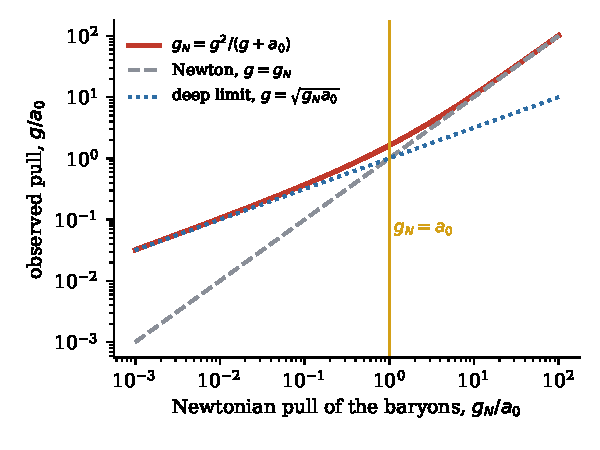
\includegraphics[width=0.85\linewidth]{figures/the_law.pdf}
\caption{The law (red) between its two limits: Newton at high acceleration (grey dashed) and $\sqrt{\gbar a_0}$ at low acceleration (blue dotted). The bend happens at $\gbar\approx a_0$, the only scale in the problem.}
\end{figure}

Equivalently, in Milgrom's notation $g\,\mu(g/a_0)=\gbar$, the law uses
\begin{equation}
\mu(x)=\frac{x}{1+x},
\end{equation}
the ``simple'' interpolating function, which Famaey and Binney found to fit the Milky Way well in 2005.

\fig{interp_family}{The shape knob nobody counts. Four interpolating functions with the same two limits differ by up to 0.1\,dex near the transition. Choosing the simple form is a decision made once; counted honestly, it's a meta-knob.}


\section{Whose idea is it?}

Let me be completely clear about credit, because this book would be worthless if it weren't.
\begin{itemize}
\item The relation between $g$ and $\gbar$, with a single acceleration scale, is \textbf{Milgrom's} modified Newtonian dynamics, proposed in 1983. The simple form of the interpolating function is well known in the MOND literature.
\item The nearness of $a_0$ to $cH_0$ and to $c^2\sqrt\Lambda$ is also \textbf{Milgrom's} observation, from his first papers and again in 1999.
\item The proposal that the scale is tied to the \textbf{dark energy density} was made by \textbf{Limbach, Psaltis and \"Ozel} in 2008.
\end{itemize}
What this programme adds is a particular coefficient, $\kappa=\tfrac12$, which is fitted; a reconstruction of how the scale should change over cosmic time from raw expansion data (Chapter~13); a graded comparison with every rival I could think of (Part~II); and a public record of every failure (Chapter~12).

\section{The numbers}

Using $\rhoDE=5.84\times10^{-27}\,\mathrm{kg\,m^{-3}}$, which corresponds to the dark energy share and expansion rate of the standard reading of the expansion history,
\begin{equation}
a_0=\tfrac12\,c\sqrt{G\rhoDE}=\tfrac12\,(3.00\times10^8)\sqrt{3.90\times10^{-37}}=9.36\times10^{-11}\ms,
\end{equation}
since $G\rhoDE=(6.674\times10^{-11})(5.84\times10^{-27})=3.90\times10^{-37}\,\mathrm{s^{-2}}$.

A few worked examples from the law's limits:
\begin{center}
\begin{tabular}{lrr}
\toprule
baryonic mass & flat speed $v_f=(GMa_0)^{1/4}$ & $r_M=\sqrt{GM/a_0}$\\
\midrule
$10^9\Msun$ (a dwarf) & $59\kms$ & 1.2 kpc\\
$10^{10}\Msun$ & $106\kms$ & 3.9 kpc\\
$6\times10^{10}\Msun$ (Milky Way-ish) & $165\kms$ & 9.4 kpc\\
$10^{11}\Msun$ & $188\kms$ & 12.2 kpc\\
\bottomrule
\end{tabular}

\smallskip
{\footnotesize $r_M$ is the radius at which a point mass's Newtonian pull falls to $a_0$. Real discs are extended, so treat it as a scale, not a boundary. Speeds are on the canonical footing.}
\end{center}

\section{Two footings, never pooled}

There's a subtlety that every honest report of this law has to carry. ``The dark energy density'' and ``the critical density'' differ by the factor $\Omega_\Lambda\approx0.685$, and the programme has always reported results on both readings. They're called \emph{footings}.

\textbf{Canonical footing.} $\kappa=\tfrac12$ on the dark energy density: $a_0=9.3603\times10^{-11}\ms$.

\textbf{Alternative footing.} $\kappa=\tfrac12$ on the critical density $\rho_c=3H_0^2/8\pi G$:
\begin{gather}
a_0=\frac12\,c\sqrt{G\rho_c}=\frac12\,c\sqrt{\frac{3H_0^2}{8\pi}}=\frac{cH_0}{2\sqrt{8\pi/3}}\equiv\frac{cH_0}{Z},\\
Z=2\sqrt{\frac{8\pi}{3}}=5.7888.
\end{gather}
With $H_0=67.4\kms\,\mathrm{Mpc}^{-1}$ this is $1.1312\times10^{-10}\ms$. This was the programme's earliest form, $a_0=cH_0/Z$, before the tie to dark energy was made explicit.

The two values differ by $1/\sqrt{\Omega_\Lambda}\approx1.21$, about $0.08\dex$. Every result is reported on both footings and they're never averaged, because averaging would hide whichever one fails. They differ in a deeper way too: the canonical footing tracks dark energy, so it stays nearly flat in redshift, while the alternative tracks the critical density and rises with $H(z)$. That's the contrast at the heart of Chapter~13.

\section{The knob is fitted}

Now the confession that every chapter after this one depends on. \textbf{$\kappa=\tfrac12$ is not derived.}

The programme's record lists about 550 attempts to derive or select it: from horizon thermodynamics, from entropy arguments, from field equations, from symmetry. None succeeded. A closure analysis (the lane called KC1) reduced every route to the same missing piece. Setting $\kappa=\tfrac12$ is mathematically the same as asserting that some physical length is exactly $c/\sqrt{G\rho}$, and no field equation on record supplies that length. A screen of sixteen further premises found none that does (KC2). Another lane (KF1) found routes that give $\tfrac12$, 1.447 or 1.772 depending on which length you choose, and only the length with no field equation behind it gives $\tfrac12$.

So it's a knob. One knob. I set it.

\section{Does the data even pick \texorpdfstring{$\tfrac12$}{1/2}?}

Not decisively. Here's the profile likelihood over 175 SPARC galaxies, which asks how much worse the fit gets as $a_0$ is moved away from its best value (with galaxy-to-galaxy correlations included in the error estimate):

\begin{center}\small
\begin{tabular}{@{}lrrr@{}}
\toprule
choice of $a_0$ & value ($\ms$) & $\Delta\chi^2$ & significance\\
\midrule
free best fit & $1.0766\times10^{-10}$ & 0 & --\\
$\kappa=\tfrac12$ on $\rhoDE$ (canonical) & $9.36\times10^{-11}$ & 63.90 & 1.82$\sigma$\\
$\kappa=\tfrac12$ on $\rho_c$ (alternative) & $1.1312\times10^{-10}$ & 7.04 & 0.60$\sigma$\\
Milgrom's $cH_0/2\pi$ & $1.042\times10^{-10}$ & 5.34 & 0.53$\sigma$\\
\bottomrule
\end{tabular}
\end{center}

\fig{footings}{Candidate values of $a_0$ on SPARC, with their distance from the free best fit in clustered standard deviations. Milgrom's $cH_0/2\pi$ and the alternative footing sit closer to the best fit than the canonical $\kappa=\frac12$; a $2\pi$ horizon form on $\rho_{\rm DE}$ sits furthest.}

\begin{honestbox}[Milgrom's value fits at least as well]
On SPARC alone, Milgrom's own $cH_0/2\pi$ fits at least as well as my canonical $\tfrac12$, and the alternative footing sits between. The data can't settle the coefficient yet. To tell $\tfrac12$ from $0.461$, the value a $2\pi$ horizon form gives on the dark energy footing, at three standard deviations, you'd need $a_0$ to 2.8 per cent. The shared galaxy-mass floor, the uncertainty that every galaxy shares through stellar mass-to-light ratios and distances, is about 9.5 per cent, and the best case with the dark energy density is about 5 per cent. More archive data won't fix this; only new observations will. And Chapter~8 showed that plausible systematic corrections move the fitted scale by up to $\pm0.15\dex$.
\end{honestbox}

So why $\tfrac12$ at all? Because it's simple, because it puts the scale on the dark energy density with no $\pi$s floating around, and because it was the programme's starting hypothesis. Those are reasons to \emph{choose} it, not evidence that it's right. What makes the choice interesting is what it commits the law to, and that's Part~V.

\section{The honest knob count}

The cleanest way to finish this chapter is with the same knob accounting I applied to everyone else.

\begin{knobbox}{The law's control panel}
\begin{tabular}{@{}lp{6cm}@{}}
\toprule
item & status\\
\midrule
$\kappa$ & \textbf{1 global knob}, fitted; 6.6 bits\\
the scale $\rhoDE$ & not a knob: measured by the expansion of the universe, independently of galaxies\\
the function $\mu(x)=x/(1+x)$ & a shape choice made once (the simple MOND form); counted as a meta-knob\\
per-galaxy $\Upsilon$, distance, inclination & nuisance knobs, paid by \emph{every} theory including \LCDM; fixed at 0.5 and 0.7 in the fried chicken comparison\\
a Solar System screen & needed; the action adopted for it (v3s, Chapter~11) brings its own structure, and $a_0$ still enters it by hand\\
clusters, CMB & \textbf{not covered}; no knob offered (Chapter~12)\\
\bottomrule
\end{tabular}
\end{knobbox}

That last row matters. A theory with one knob that explains only galaxies isn't comparable, knob for knob, with a theory with six knobs that explains the CMB. What the one knob \emph{does} explain, it explains with almost no freedom. Let's see what that buys.

\chapter{What One Knob Buys}

\epi{Twelve knobs to imitate it. One knob to be it.\\ Here's the receipt.}

\section{The scoreboard, read kindly}

This chapter collects what the law gets right. Chapter~12 collects what it gets wrong, and that chapter is longer. Before the good news, three ground rules, so that nobody (including me) gets carried away.

First, most of the comparisons below are against the programme's own \emph{native halos}: dark-matter-like halos it built and graded on the same footing, then retired in November 2026. They are not \LCDM\ hydrodynamic simulations. A win against them is a win against them.

Second, every number is from a frozen grade, the programme's final scorecard (FG1) or a named lane, and a clean-room regrade reproduced FG1's table (289 match, 6 close, 0 disagree). That regrade mainly tested the code, not the independence of the definitions.

Third, none of this says the data favour the law over \LCDM. It says what one knob does.

\section{Win 1: galaxies stay tight}

On the SPARC sample, letting each galaxy's stellar mass-to-light ratio float inside a line of 0.50 to 0.80 (the nuisance knob every theory pays), the law's residuals have an rms of $\mathbf{0.0541\dex}$, about 13 per cent, at a median $\Upsilon$ of 0.52. The native halos, given the same freedom, scatter by $0.0682$ and $0.0694$.

\begin{honestbox}[A caution on the $\Upsilon$ line]
The 0.50--0.80 line was first written for this law, and its lower edge is a stellar-population model's central value, not a measurement. Passing it is weaker than it looks. Chapter~12 sets it against measured stellar masses, where the law does worse.
\end{honestbox}

\fig{wins_panels}{Four of the law's wins on one page. Top left: scatter on SPARC, the law against two versions of the programme's native halos. Top right: the median offset $E$ on LITTLE THINGS dwarfs. Bottom left: 63 galaxy groups, where $|Z|<2$ passes, on both footings. Bottom right: the law's $a_0$ measured on MeerKAT galaxies against SPARC, inside a line of $\pm0.15\dex$.}

\section{Win 2: no tilt with speed}

If the law's scale were wrong, or if galaxies of different masses needed different scales, the residuals would drift with rotation speed. They don't: the tilt is $+0.02$ on the canonical footing and $-0.02$ on the alternative, both consistent with zero.

\section{Win 3, the strongest: surface brightness}

Here's the result I'd put first if I could only keep one.

Take galaxies that rotate at the same speed, 60 to 120\kms, so they have about the same mass. Some are compact and bright; some are spread out and dim. Ask whether the law's residuals depend on surface brightness. If the extra gravity came from a halo whose properties are set by the galaxy's \emph{mass}, the dim galaxies and the bright ones would need the same halo, and the residuals would tilt with surface brightness. The law, which responds to the local $\gbar$ at each radius, has no such tilt built in.

The data: the law's residual slope with surface brightness is $\mathbf{-0.016\pm0.061}$ per dex (alternative footing $-0.023\pm0.063$), flat. Every version of the programme's mass-set halos tilts, at $-0.17$ to $-0.29$ per dex.

\fig{sb_tilt}{The strongest result: at fixed rotation speed, the law's residuals don't care about surface brightness (black, both footings), while halos set by mass tilt by $-0.17$ to $-0.29$ per dex (red band).}

This is the shape problem of Chapter~4 seen in real data. Recall Figure~\ref{fig:levelshape}: one halo, two discs, two tracks. The law puts every disc on one line, and so do the galaxies.

\begin{honestbox}
That's a real discriminator on the data used, but only between the law and the halos tested. A \LCDM\ halo whose properties depend on surface density as well as mass, like the R7 recipe of Chapter~4, could in principle remove the tilt; that's what its extra knobs were for.
\end{honestbox}

\section{Win 4: dwarfs}

Dwarf galaxies are gas-rich and dark-matter-dominated, which makes them a sharp test: there's little stellar mass to hide behind. On the LITTLE THINGS sample of dwarf irregulars, the law's median offset is $E=-0.025$ (alternative $-0.064$). The native halos' is $+0.138$.

\section{Win 5: groups}

Small groups of galaxies sit between single galaxies and clusters. On 63 groups the law reads $Z=+0.31$ on the canonical footing and $-0.31$ on the alternative, well inside the $\pm2$ pass line. That's worth noting, because the next step up in mass, the clusters, is where the law falls over.

\section{Win 6: the same scale in a different sample}

If $a_0$ is a property of the universe, galaxies measured with a different telescope and a different team should give the same value. The law's scale fitted on MeerKAT galaxies sits $+0.032\dex$ from its SPARC value, inside a line of $0.15\dex$ set in advance.

\section{Win 7: the shape of lensing around galaxies}

Weak lensing around isolated galaxies probes their gravity out to a megaparsec, far beyond the visible disc. On KiDS-1000 lenses, the law's \emph{shape} is preferred over the best native halo by $\Delta\chi^2=+366$. The law predicts, in its deep regime, an excess surface density that falls as $1/R$ out to large radius, with no edge.

\fig{delta_sigma}{What a lensing survey measures, around a toy galaxy of $5\times10^{10}M_\odot$. Stars and gas alone (blue dashed) fall as $1/R^2$. The law (red) adds a phantom mass whose signal tends to $\sqrt{GMa_0}/4GR$ (grey dotted). An untruncated NFW halo (black) is similar in size at 100\,kpc and bends down further out. The difference in shape is what KiDS sees.}

\begin{honestbox}
Shape, not amplitude. The law's lensing amplitude depends on galaxy colour and on how much hot gas is counted, and inside 0.3\,Mpc the data sit about $0.09\dex$ above the law under every estimator on record. No tested model, including the law, fits these profiles in absolute terms. Chapter~12 has the details.
\end{honestbox}

\section{Win 8: Tully--Fisher for free}

The baryonic Tully--Fisher relation, $M_b=v_f^4/Ga_0$, isn't a fit in the law; it's a consequence. The slope of exactly 4 and the zero point both follow from the one knob. Milgrom predicted this in 1983, so the credit is his; the law inherits it.

\fig{btfr}{The baryonic Tully--Fisher relation from the law's deep limit, on both footings. The slope of 4 is not adjustable. The zero point is set by $a_0$, so it's set by $\kappa$ and by the dark energy density.}

\section{Win 9: same fit, one knob}

Now the comparison the book has been building. Chapter~4 found that, on the observed rotation curves at fixed $\Upsilon$, the twelve-knob recipe and the law are indistinguishable. Here it is again, with the complete recipe of Chapter~7 added.

\fig{knob_economy}{Knob economy on the observed rotation curves at fixed $\Upsilon$. All five sit inside a band of 0.003\,dex, smaller than this statistic can resolve. The recipes got there by being tuned to the law; the law got there with one knob set once.}

\begin{knobbox}{The economy, stated carefully}
Five models, the same fit to the data. The law uses one knob, $\kappa$, which carries 6.6 bits. The recipes use 9 to 26 knobs, and they got their fit by being tuned \emph{to the law}, not to the data. Remove the law and they have nothing to aim at. That's the honest content of ``one knob versus twelve'': not a better fit, but the same fit from a much smaller control panel, which is what a law looks like when it has captured something.
\end{knobbox}

\section{Win 10: an action, in a stated scope}

A formula for accelerations isn't a theory of gravity. A theory needs an \emph{action}, a single expression from which all the equations of motion follow, including how light bends, how gravitational waves travel and what happens in the Solar System. That last one is a real problem for the law as written. Its strong-field limit, $g\approx\gbar+a_0$, leaves a constant extra pull of order $a_0$ even where gravity is strong, and in the Solar System the Cassini spacecraft's tracking rules that out (Chapter~12). The law needs a \emph{screen}: something that switches the modification off in strong fields.

On 4 November 2026 I adopted, as the action for the law, a theory the programme calls v3s. It's a version of the Khronon idea of Blanchet and Skordis, a field that picks out a preferred slicing of spacetime into moments of time, with a ``switched stiffness'' that provides the screen. I adopted it in a limited scope: isolated galaxies, the Solar System, galaxy lensing and gravitational waves.

The gates it rests on:
\begin{itemize}
\item \textbf{Every action class graded} (AX1): no unscreened class gives the law and passes the Solar System; only v3s's screening length does.
\item \textbf{Solar System} (C6P): a clean pass, with the Cassini signal at least $4.8\times10^7$ times inside the bound.
\item \textbf{Post-Newtonian parameters}: $\gamma=\beta=1$ derived from the action, as in general relativity.
\item \textbf{Gravitational-wave speed}: $c_T=c$, $|\Delta v/c|\le5.1\times10^{-32}$, comfortably inside the limit set by the 2017 neutron-star merger.
\item \textbf{Galaxy lensing equals dynamics}: KiDS amplitude $A=1.129\pm0.206$, which has little power.
\item \textbf{Health}: no ghost or gradient instability; force signs, dwarf virials and planetary bounds pass on both footings (VH1).
\end{itemize}

\fig{v3s_tiles}{The gates behind v3s's scoped adoption. Two items are undecided on numerics, and clusters and the CMB are outside the scope, where its failures stand.}

\begin{honestbox}[What the adoption doesn't do]
v3s supplies no mass for clusters or the CMB, and the failures there stand. Two checks are undecided on numerics. Four items are asserted, not shown: post-Newtonian corrections don't flip signs, the Sun is at rest in the Khronon frame, the solar interior is uniform, and the theory is well-posed nonlinearly. The constraints act instantaneously. And $a_0=\kappa c\sqrt{G\rhoDE}$ is put in by hand, not derived from the action. This is the programme's own version of a Khronon theory; it doesn't test the published theory.
\end{honestbox}

\section{The receipt}

Here's the law's row on the final scorecard, the part that passes:

\begin{center}\small
\begin{tabular}{@{}lll@{}}
\toprule
line & result & note\\
\midrule
SPARC scatter & pass, 0.0541 dex & $\Upsilon$ line written for the law\\
tilt with speed & pass, $+0.02$ & both footings\\
LITTLE THINGS dwarfs & pass, $E=-0.025$ & \\
63 groups & pass, $Z=+0.31$ & alt $-0.31$\\
KiDS isolated lenses & pass on shape & amplitude open\\
surface brightness & flat, $-0.016\pm0.061$ & halos tilt\\
MeerKAT $a_0$ & $+0.032\dex$ & line 0.15\\
\bottomrule
\end{tabular}
\end{center}

That's a lot of galaxy physics for one knob. It's also the same row that, read to the right, fails clusters, X-COP, the Local Group dwarfs, the Milky Way, the DiskMass discs and IC~1613. Time to read to the right.

\chapter{Where One Knob Isn't Enough}

\epi{A book about counting knobs that doesn't count its own\\ is a sales brochure.}

\fig[1.0]{plate_wall}{The wall. Each red brick is a place where one knob isn't enough, and every one of them is in this chapter: clusters, the microwave background, a stubborn dwarf, the Milky Way's vertical pull, stellar masses, disc weighings, the Solar System without a screen, the matter term, and a published high-redshift rise.}


\section{Reading the row to the right}

Here is the programme's final scorecard, FG1, frozen on 1 November 2026. It grades five candidates, four versions of a cold sector the programme built and then retired, and the law alone (C4), on eleven lines. I'm showing all five because the cold sector was my attempt to cover exactly the places where the law fails, and it failed too.

\fig{fg1_heatmap}{The final grade. Row C4 is the law with nothing added. Rows C1--C3 and C5 are versions of a cold dark energy sector the programme built to cover clusters and the CMB, graded on measured data and retired on 1 November 2026. No row passes everything. The lines aren't independent, so no winner is declared.\label{fig:fg1}}

The law's row passes the galaxy lines and fails six: the cluster keys, X-COP, the Local Group dwarfs, the Milky Way, the DiskMass discs and IC~1613. Add the CMB, which isn't on this table because the law can't even compute it, and the Solar System, where the law needs a screen it doesn't contain. Let's go through them.

\section{Loss 1: galaxy clusters}

Clusters are the oldest problem for modified dynamics, older than this programme by decades, and the law inherits it whole.

\textbf{X-COP.} For seven clusters with excellent X-ray data, the hydrostatic mass, the mass needed to hold the hot gas up against its own pressure, is \textbf{2.93 times} what the law provides from the visible baryons (alternative footing 2.72). All seven come up short. If the hydrostatic masses are biased high by $0.12\dex$, a common worry, the shortfall is still 2.23 (2.06).

\textbf{Shear around 318 clusters.} Using measured gas from eROSITA and raw lensing shear from KiDS, the law is short by a factor $A=1.91\pm0.12$ between 0.5 and 1.2\,Mpc (alternative $1.75\pm0.11$) and matches, $A=1.01\pm0.09$, between 1.2 and 3\,Mpc. On the measured chain it fails 10 of 15 keys on both footings.

\fig{clusters}{Clusters. Left: on X-COP, hydrostatic masses exceed the law's by a factor near 3, and near 2 even if the hydrostatic masses are biased. Right: lensing shear around 318 eROSITA clusters needs about twice the law inside 1.2\,Mpc and agrees further out.}

\textbf{What's missing, described.} Inside about $R_{500}$ the deficit is near 8 times the gas mass at 0.2--0.5\,$R_{500}$ and 5 times at 0.5--1\,$R_{500}$, with no detected mass dependence and no preferred scale found. The outer shear grows with gas mass as $M_{\rm gas}^{0.90\pm0.21}$, against the law's 0.47 and Newton's 0.84. So the agreement in the outer bin is an average over a slope the law gets wrong.

\fig{cluster_deficit}{What clusters are missing, relative to their hot gas. Inside about $R_{500}$ the law leaves a deficit near eight times the gas mass in the inner bin and five times further out. That's a description, not a mechanism.}



\fig{outer_shear_slope}{How outer shear grows with gas mass. The measured slope is $0.90\pm0.21$; the law predicts 0.47, Newton 0.84. The law's good average amplitude at large radius hides a slope it gets wrong.}



\begin{knobbox}{A knob I tried, and didn't adopt}
The obvious patch is a gas term: boost the law in proportion to the local gas acceleration,
\[
g=g_{\rm law}\left(1+\theta\,k\,\frac{g_{\rm gas}}{a_0}\right),
\]
with $k$ fitted on clusters. With $k=13.29$ (alternative 14.25), fitted on four X-COP clusters, the canonical cluster keys go from 10 of 15 to 14. But that's fragile: it holds only for $k$ between 12.87 and 15.09, no value gives 15 of 15, it breaks discs unless a switch turns it off there (and then it passes largely by construction), and there's no action behind it. On the Bullet Cluster's lensing map, every version tied to present gas puts the mass in the wrong place, because the observed lensing peaks sit on the galaxies, not on the gas. The frozen label is KEYS FAIL. That would have been knob number two, and it didn't earn its place.
\end{knobbox}

\fig{k_window}{Why the gas-term knob failed. Each bar is the range of $k$ that one cluster test allows. One test needs $k$ below 7.2; the others need it above 8.8 or 12.9. No single setting satisfies all three, so no value of the knob gives 15 of 15.}



\section{Loss 2: the cosmic microwave background}

This is the big one. The law's scale $a_0$ doesn't appear in the linear equations of a uniform expanding universe, so the law can't change the background expansion. It can act on the perturbations, and the potentials that CMB lensing maps between redshifts 0.5 and 2.33 have gradients of 0.003 to 0.22\,$a_0$, inside the law's regime. So the question is fair.

The answer is bad. Run on the cosmic web from a start with baryons only and no cold component, the law gets the CMB lensing spectrum wrong in \emph{shape}, not just size. As QUMOND on the peculiar field it gives about 14 times the measured lensing at multipole $L\approx28$ and 0.08 times at $L\approx377$. A baryons-only start has had its small-scale fluctuations erased by photon diffusion (Silk damping), and the law boosts the largest scales most. Letting $a_0$ track evolving dark energy, as the law says it should, lowers the whole spectrum by about half without changing its shape. A screening term put in by hand removes the large-scale excess but leaves the spectrum 1.5 to 7 times low above $L\approx100$.

\fig{cmb_lensing_shape}{The law alone against CMB lensing: too much on large scales, far too little on small ones. Two points from the graded run, joined to show the shape. Tracking dark energy halves it (gold); hand-added screening (blue band) still falls short above $L\approx100$. ``1'' would be a match.}

\begin{honestbox}[The record has no CMB pass without a dust-like component]
With a component that behaves at linear order like cold dark matter ($w=0$, no sound speed), a window exists. The programme built one, a gravitating ``cold dark energy'' sector, explicitly not a particle, and graded four versions on measured data. All four fail somewhere (Figure~\ref{fig:fg1}). Two walls stopped it: whatever behaves as dust in the CMB falls into spiral galaxies and contracts with them, which the rotation curves don't allow; and the outer shear around clusters, on measured gas, misses at $Z=+4.41$. The sector was retired on 1 November 2026. \textbf{The law offers no replacement, and I don't claim it needs none.} This is exactly where \LCDM's six knobs shine.
\end{honestbox}

\section{Loss 3: lensing around galaxies, in detail}

Chapter~11 counted the \emph{shape} of galaxy lensing as a win. The \emph{amplitude} isn't. Inside 0.3\,Mpc the data sit above the law by $+0.0887\dex$ (alternative $+0.0500$) under every grader on record, and no single swap of estimator brings the full-profile grade inside $|Z|=2$. The hot gas measured through the kinematic Sunyaev--Zel'dovich effect, mostly at 200--500\,kpc, doesn't close the gap.

The amplitude also depends on colour. Red lenses read well above the law and blue lenses slightly below. One gas rule for both colours can't bring red within 2$\sigma$ without pushing blue over.

\fig{lens_colour}{Galaxy lensing amplitude relative to the law, for red and blue lenses, as more of the baryon inventory is counted. Red stays 4.87$\sigma$ above 1 even with measured hot gas. No tested model fits these profiles in absolute terms.}

\section{Loss 4: IC 1613}

One nearby dwarf galaxy, IC~1613, doesn't fit. The law's offset is $E=-0.593$, $Z=-7.9$, and it fails under every inclination the data allow. That $Z$ has no velocity error in it; with 15 per cent on the velocities the base is $-3.94$, and $-2.35$ to $-2.83$ at the central inclinations of an independent analysis. Only a much more face-on disc would close it: $E=0$ needs an inclination of about $22^\circ$, against central estimates of 34 to 38. A disturbed gas disc is a live explanation that nobody has computed. One galaxy disfavours a law; it doesn't exclude it. But it's on the list.

\section{Loss 5: the Local Group's dwarfs}

The satellites of the Milky Way and Andromeda are the most dark-matter-dominated systems known, and several classes of them miss.

\fig{dwarf_z}{Local Group dwarf classes against the law ($Z$; inside $\pm2$ passes). Ultra-faint satellites of the Milky Way miss badly, and including the host galaxy's external field, which modified dynamics says should matter, makes it worse.}

The Milky Way's ultra-faints read $Z=+5.22$; Andromeda's bright satellites $+2.20$ and its others $+2.29$. Adding the external field from the host, which in MOND-type theories weakens a satellite's internal boost, makes it worse: $+6.76$ and $+3.97$. Worse still, at fixed luminosity the data are flat in host field ($-0.05\pm0.19$ per dex) where the external-field theory predicts $-0.76$. Listed systematics (binary stars, tides, membership, heating) don't close it: a central stack of them leaves the ultra-faints at $+5.08$.

\section{Loss 6: the Milky Way's vertical pull}

The law gives the in-plane force. To test the Milky Way, you also need the force perpendicular to the disc, $K_z$, which the law as written doesn't supply. The two standard field-equation forms (AQUAL and QUMOND) can't reach the measured $K_z$ at the Sun's position inside the priors: the lowest they get is 75.9 against an upper line of 70.8. A simpler rule passes only in a few corners of parameter space and still misses the scale length. FG1 counts it as a fail.

\section{Loss 7: measured stellar masses}

The law asks for stellar mass-to-light ratios of 0.62 and 0.65 in galaxies rotating at 60--150\kms. Stellar masses from the GSWLC catalogue give 0.277 and 0.304 for the same galaxies, a miss at $Z=+3.4$ and $+5.6$. These are estimators against a different photometric band, not a direct measurement, and offsets, distances and inclinations don't carry the difference. The law wants about twice the stellar mass the photometry suggests.

\fig{upsilon_compare}{Stellar mass-to-light ratios in two bins of rotation speed: what the law needs (red) against what stellar masses from the GSWLC catalogue give (blue). The gaps are $Z=+3.4$ and $+5.6$.}



\section{Loss 8: disc thickness}

The DiskMass survey measured vertical stellar velocity dispersions in face-on discs, which weigh the disc directly. On the law's own form, the ratio that should be near 1 reads 1.239 (alternative 1.204), outside the 0.90--1.10 line. Corrections for which stars are being measured could move it inside, but the sources' own tables span a wide range. This one is open, and graded as a fail.

\section{Loss 9: the Solar System}

As written, the law leaves a nearly constant extra pull of order $a_0$ even in strong fields, and in the Solar System that shows up as an anomalous quadrupole in the Sun's gravitational field, which radio tracking of the Cassini spacecraft at Saturn constrains. The unscreened law fails that constraint by 2.44 to 4.59 times (alternative 2.85 to 5.19). Every unscreened action class in the record fails it, by 1.69 to 5.18 times. Only v3s, with its screening length, passes.

\fig{solar_system}{The Cassini constraint. Unscreened, the law and every unscreened action fail by factors of 2 to 5. With v3s's screen the signal drops more than seven orders of magnitude below the line. The screen is the price of the Solar System, and it's paid in v3s's extra structure.}

\section{Loss 10: the matter term}

There's a quieter problem underneath everything. The law takes $\rhoDE$ from the expansion history, and that history contains a matter term several times larger than the baryons. The law doesn't explain that term. Even the redshift band of Chapter~13 uses $\rho_m(z)=\omega_m(1+z)^3$ with a cold mass taken from the CMB. With only positivity, and no CMB or Hubble-constant input, that band's own check fails. So the cleanest prediction in this book isn't entirely free of the sector the programme retired.

\section{The 96-row list}

The programme also built a harness that grades any proposed $g$ on one list of 96 rows. The rows are correlated in blocks and many are disputed, so the counts don't rank anything. They do show how much of the universe each candidate can even attempt.

\fig{rq3_counts}{The 96-row list. Green pass, red fail, gold depends on the form, grey not computable. Newton's 10 passes show how little those rows ask. For the law, 38 rows need an action or a Boltzmann calculation it doesn't have. These counts don't rank the candidates.}

\section{What a successor must do}

From the failures, the programme wrote down twelve requirements that any theory replacing the law (or completing it) has to meet:

\begin{center}\small
\begin{tabular}{@{}rp{3.1cm}p{4.0cm}@{}}
\toprule
\# & must & the law\\
\midrule
1 & keep galaxies tight & \textbf{0.0541 dex}\\
2 & stay flat with surface brightness & \textbf{$-0.016$}\\
3 & sit on $\Upsilon$ at every speed & 0.52 (alt 0.44)\\
4 & little net contraction in spirals & not needed\\
5 & fit dwarfs & \textbf{$-0.025$}; ultra-faints $+5.08$\\
6 & fit IC 1613 & $-0.593$\\
7 & fit the Milky Way & AQUAL, QUMOND infeasible\\
8 & fit isolated lenses & shape preferred; 0.09 dex short inside 0.3 Mpc\\
9 & add mass in cluster cores & $A=1.91$\\
10 & match outer cluster shear & slope 0.47 against 0.90\\
11 & act as dust in the CMB & no cold term\\
12 & have an action & met in a scope only (v3s)\\
\bottomrule
\end{tabular}
\end{center}

The collisions are the interesting part. Rows 4 and 11 pull against each other: dust in the CMB falls into galaxies. Rows 1--3 and 10 pull against each other: the amount of extra gravity needed runs from about 0.8 of a native halo's in SPARC to 1.2--1.8 in clusters. Rows 7 and 8: systems of the same mass want different things. None of this is a theorem, but every route the programme tried ran into one of these collisions.

\fig{collision_graph}{The twelve requirements as a network. Red lines join requirements that pull against each other: dust in the microwave background against little contraction in spirals; tight galaxies against outer cluster shear; the Milky Way against isolated lenses.}



\section{The honest count}

So here's the law's control panel, with the losses included.

\begin{knobbox}{The law, all in}
One knob ($\kappa$, fitted). One shape choice ($\mu=x/(1+x)$). One adopted action (v3s) in a scope, with its screening structure and with $a_0$ still put in by hand. Galaxies: tight, flat with surface brightness, dwarfs and groups passing. Clusters: short by a factor of 2 to 3. CMB: nothing. Solar System: only with the screen. Local Group dwarfs, IC~1613, the Milky Way's vertical force, measured stellar masses, disc weighings: fail or open.
\end{knobbox}

One knob explains a remarkable amount about disc galaxies. It doesn't explain the universe. \LCDM\ explains the universe's large-scale structure with six knobs and needs dozens more to make a galaxy look like the law. My law makes a galaxy look like the law with one knob and can't make a universe.

You might think that's a draw, or a loss on points. But there's one more thing the one knob does, and it's the reason this book exists. It makes a prediction that no one can tune.


\part{The Knob That Can't Be Turned}
\chapter{The Knob That Can't Be Turned}

\epi{Every theory in this book has a dial somebody could reach for.\\ This one is welded shut, and the universe holds the key.}

\fig[1.0]{plate_locked_knob}{The knob that can't be turned. Once $\kappa$ is set by galaxies today it cancels from the ratio, and the key to $a_0$'s history is held by expansion surveys that never look at a rotation curve.}


\section{Where \texorpdfstring{$\kappa$}{kappa} goes to disappear}

Here's the law's scale again, now written as a function of cosmic time:
\begin{equation}
a_0(z)=\kappa\,c\sqrt{G\rhoDE(z)}.
\end{equation}
Divide by today's value:
\begin{equation}
\boxed{\;\frac{a_0(z)}{a_0(0)}=\sqrt{\frac{\rhoDE(z)}{\rhoDE(0)}}\;}
\end{equation}
The knob is gone. $\kappa$ cancels, $c$ cancels, $G$ cancels. What's left is a ratio of dark energy densities at two times, and that ratio is measured by surveys of the expansion of the universe (baryon acoustic oscillations, supernovae) that have nothing to do with how galaxies rotate. Nobody gets to set it with galaxy data. Not me, not a referee, not a rival.

That's the knob that can't be turned. Once $\kappa$ is fixed by galaxies today, the law's entire history is fixed by cosmology. If dark energy is a cosmological constant, $a_0$ is exactly the same at every redshift. If dark energy evolves, $a_0$ evolves with it, by an amount you can compute in advance.

\section{What evolving dark energy does to \texorpdfstring{$a_0$}{a0}}

\begin{mathbox}{From $w(z)$ to $a_0(z)$}
Energy conservation for a fluid with pressure $p=w\rho c^2$ in an expanding universe gives
\[
\frac{d\rho}{dt}=-3H(1+w)\rho\quad\Longrightarrow\quad\frac{\rhoDE(a)}{\rhoDE(1)}=\exp\left[3\int_a^1\frac{1+w(a')}{a'}\,da'\right],
\]
where $a=1/(1+z)$ is the scale factor. For the common parameterisation $w(a)=w_0+w_a(1-a)$, the integral is elementary:
\[
\frac{\rhoDE(z)}{\rhoDE(0)}=(1+z)^{3(1+w_0+w_a)}\exp\left(-\frac{3w_az}{1+z}\right).
\]
So the law predicts, with no galaxy input at all,
\[
\frac{a_0(z)}{a_0(0)}=(1+z)^{\frac32(1+w_0+w_a)}\exp\left(-\frac{3w_az}{2(1+z)}\right).
\]
For $w_0=-1$, $w_a=0$ this is exactly 1.
\end{mathbox}

Try an illustrative evolving case, $w_0=-0.75$ and $w_a=-0.8$, roughly the kind of values recent surveys have hinted at (these are for illustration, not a fit):
\begin{center}
\begin{tabular}{lccccc}
\toprule
$z$ & 0.5 & 1 & 1.5 & 2 & 2.33\\
\midrule
$a_0(z)/a_0(0)$ & 1.068 & 1.029 & 0.965 & 0.899 & 0.858\\
\bottomrule
\end{tabular}
\end{center}
It rises a little, then falls. Each number came from cosmology alone.

Figure~\ref{fig:w0wa} in Chapter~2 shows where this illustrative case sits in the dark energy knob plane. Every point in that plane gives its own $a_0(z)$ history, and none of them needs a galaxy knob.


\fig{cpl_family}{Twenty possible dark energy histories (grey), each giving a different $a_0(z)$ with zero galaxy knobs. The surveys pick the curve; the law has to follow it. A cosmological constant gives the flat red line. The rival rule $a_0\propto H(z)$ (blue) rises steeply.}

\section{The band}

The programme reconstructed $\rhoDE(z)$ from raw baryon-acoustic and supernova data with a stated distance ruler (the lane called CFG689), and converted it to the law's prediction. At 68 per cent confidence:
\begin{center}
\begin{tabular}{lccc}
\toprule
$z$ & 1 & 1.5 & 2.33\\
\midrule
the law, $a_0(z)/a_0(0)$ & 0.91 [0.76, 1.03] & 0.94 [0.71, 1.12] & 0.91 [0.33, 1.21]\\
rival, $a_0\propto H(z)$ & 1.76 & 2.35 & 3.49\\
\bottomrule
\end{tabular}
\end{center}
These are predictions from the measured dark energy density, not measured galaxy values. Constant dark energy isn't rejected by the same data (1.97$\sigma$).

\fig{a0z}{The prediction that can't be tuned. Red: the law's band from the measured dark energy history. Blue: the rival $a_0\propto H(z)$ from the same reconstruction. Dark bar: the tuned \LCDM\ recipe of Chapter~8 put in earlier universes. Gold: one published measurement at face value (see below).}

\begin{honestbox}[What the band rests on]
The band isn't free of the retired cold sector's input. It takes the matter density as $\rho_m(z)=\omega_m(1+z)^3$, with a cold mass taken from the CMB, and with positivity alone, no CMB and no Hubble constant, its own check fails. The law doesn't explain that matter term (Chapter~12).
\end{honestbox}

\section{Everybody else's scale climbs}

Now line up every acceleration scale from Part~II and ask what it does by $z=2.33$, about eleven billion years ago.

\fig{redshift_rise}{Every scale in the book at $z=2.33$, relative to today. Halo-based scales follow the expansion rate or the matter density and climb by factors of 1.3 to 5. The law follows the dark energy density and stays near 1. Only a recipe with hand terms typed in to imitate the law stays down with it.}

This is the payoff of Chapter~6. Halo accelerations are built from $G$, $M$ and $H$, so at fixed mass they grow roughly as $H^{4/3}$, and every \LCDM\ route the paper tried rises: 1.42 times for the Kaplinghat--Turner scale, 1.49 for the strongest swoop, 3.0 to 4.6 for the frozen fourteen-knob recipe. The law can't rise unless dark energy itself rises, and the measured dark energy history doesn't rise much.

\section{What to measure: Tully--Fisher in the past}

The cleanest observable is the baryonic Tully--Fisher relation, $M_b=v_f^4/Ga_0$. At fixed rotation speed, a change in $a_0$ shifts the baryonic mass by
\begin{equation}
\Delta\log_{10}M_b\big|_{v_f}=-\log_{10}\frac{a_0(z)}{a_0(0)}.
\end{equation}

\fig{btfr_shift}{The Tully--Fisher shift at fixed speed. The law (red, with its band) stays within a few hundredths of a dex of today's relation. The rival $a_0\propto H(z)$ needs galaxies about 0.25\,dex lighter at $z=1$ and 0.54\,dex lighter at $z=2.33$. The tuned \LCDM\ recipe sits lower still.}

At $z=2.33$ the law says about $+0.04\dex$; the rival says $-0.54\dex$, a factor of 3.5 in mass. That's not a subtle difference. The trouble is measuring baryonic masses of distant galaxies to a few hundredths of a dex, which nobody can yet do.

\section{The bad news first}

Before the hard part about measurement, the bad news, because it exists and it's in the record.

In 2026 the MUSE-DARK team (Ciocan and collaborators, paper III of their series) fitted the radial acceleration relation in 79 galaxies between redshift 0.33 and 1.44 and reported
\[
a_0(z\sim1)=2.38^{+0.12}_{-0.10}\times10^{-10}\ms,
\]
rising with redshift at $a_1=1.59\pm0.10$ in the same units per unit redshift (95 per cent intervals). Our band at $z=1$ on the canonical footing is $0.91\times9.36\times10^{-11}$, a factor of about 2.8 lower. An independent author, Alcock, fitted the survey's four bins as read from its figure and found a constant $a_0$ excluded at 5.3$\sigma$ if the bars are one standard deviation, and at 10$\sigma$ or more if they're 95 per cent intervals; on that reading, $a_0\propto E(z)$ is in tension too, at 4.2$\sigma$. The MUSE-DARK paper notes that frameworks tying $a_0$ to the cosmological constant are under the same pressure. That's this law. It was received before the programme's first deposit using these data, and I claim no priority on it.

\begin{honestbox}[Why I read it as not decisive, and what that reading rests on]
The survey's main fit leaves each galaxy's stellar mass free of its photometric estimate. The programme's own frozen run on a different sample of 109 galaxies (CFG262, not a direct $a_0$ measurement) found that the rise travels with the mass route: from $z=0.52$ to 1.20 the implied change is $+0.570\pm0.094\dex$ with fitted masses, $-0.115\pm0.489$ with photometric masses plus molecular gas, and $+0.036\pm0.138$ with photometric masses alone. The photometric routes are consistent with flat, and also with $H(z)$, so they rescue nothing. A redshift-dependent mass drift of 0.13--0.19\,dex would remove the rise; the survey puts its unmodelled molecular gas near 0.2\,dex, but nothing shows such a drift is present. Their companion paper finds no Tully--Fisher zero-point evolution at $z\sim1$ ($0.00\pm0.06\dex$). \textbf{On the survey's own masses, the band and the dark energy tie fail.} That reading stands until a per-galaxy reanalysis with independent baryon masses says otherwise. The programme tried that reanalysis (FN3): with the gas unmeasured, a planted rise of the survey's size still grades as consistent with the band, so the existing data cubes can't decide.
\end{honestbox}

\fig{mass_route}{Why the published rise is read as not decisive. The programme's frozen run on 109 galaxies finds the implied change in $a_0$ depends on how stellar masses are obtained: a large rise when they're fitted freely, nothing significant when they come from photometry. The answer travels with the mass route.}



\section{Why nothing on disk can decide}

The difficulty isn't the number of galaxies; it's the part of the mass error that every galaxy in a sample shares. Call it the common mode: a shared bias from the stellar-population model, the gas inventory or the distance scale, which doesn't average down.

\fig{common_mode_cartoon}{Why more galaxies don't help on their own. Left: when each galaxy's error is independent, the average of 60 lands on the truth. Right: when every galaxy shares the same bias, the average lands confidently in the wrong place.}

 The programme froze a decision rule (AT1, its arithmetic checked in the Lean proof assistant). To separate the law from $a_0\propto H$ at 3$\sigma$, the total error must be below $0.055\dex$ at $z=1$ and $0.084\dex$ at $z=2.33$. With 0.14\,dex of scatter per galaxy, the common mode $\sigma_{\rm cm}$ and the number of galaxies $N$ must satisfy, roughly,
\begin{equation}
\sigma_{\rm cm}^2+\frac{0.14^2}{N}<(\text{budget})^2.
\end{equation}
At $\sigma_{\rm cm}=0.05\dex$ the frozen rule needs 41 galaxies at $z=1$ and only 5 at $z=2.33$. At $0.075\dex$, only $z=2.33$ stays open.

\fig{decision_power}{How many galaxies it takes to decide, as a function of the sample's shared mass error, in a simplified form of the frozen rule. Near the budget the number explodes. Every high-redshift sample on disk has a common mode of 0.30 to 0.60\,dex, far off this chart.}

The programme applied the rule to every high-redshift sample it has on disk: 22 samples, 52 redshift cells. All 52 are BLOCKED, with common modes of 0.30 to 0.60\,dex and no matched local reference. That's not a failure of the law or of its rivals. It's a statement that the experiment hasn't been done yet.

\section{What would decide it}

One measurement, named but not scheduled: \textbf{a single clean deep-MOND galaxy at $z\approx2.5$ with $a_0$ measured to about 0.10\,dex}, with gas and stars weighed independently of the rotation curve. At that redshift the law and its rival differ by more than half a dex, and the tuned recipes by more. A handful of such galaxies, with a shared mass error under 0.084\,dex, would settle it.

\fig{mock_decider}{What a deciding measurement could look like (mock data, not a measurement). Five galaxies near $z\approx2.3$ with baryonic masses weighed to 0.14\,dex. The law (red) and its rival (blue dashed) are about half a dex apart, so a handful of clean galaxies would tell them apart.}



Meanwhile, three dated tests are on the calendar.

\fig{timeline}{Dated tests. The first three are scheduled data releases; none of them tests the dark energy tie directly. The last is the measurement that would.}

\textbf{ALMA U4\_28473, public 6 November 2026.} One galaxy at high redshift, with predictions frozen in PAPER66. It tests that galaxy's mass budget, not $a_0(z)$, and one disc excludes no model.

\textbf{GS4\_24110, late November 2026} (date from earlier metadata, to be rechecked). Every pairing of the alternatives tested gives at most 0.51$\sigma$ separation, so it can't decide.

\textbf{Gaia DR4, around December 2026.} Wide binary stars, separated by thousands of astronomical units, orbit each other with accelerations below $a_0$, inside the Galaxy's own field. The prediction is sealed: the law in QUMOND form, unscreened, gives a velocity ratio $\gamma_\infty=1.149$ (alternative 1.208) through the frozen pipeline. A Newtonian result at 2--30\,thousand AU would count against the bare law. (That last sentence is a reading, not a frozen line: the registered bands were written for the fuller framework, and an amendment registers a gated branch that also predicts Newton inside 30\,thousand AU.)

\fig{wide_binaries}{What Gaia DR4's wide binaries could show. Newton gives 1. The law, sealed in advance, gives 1.149. The earlier DR3 dry run's 1.205 is evidence for nothing; it was a test of the pipeline.}

\section{Why this is the point}

Every theory in this book could, in principle, reach for a knob when a measurement goes wrong. \LCDM\ can add extensions or retune feedback; the fried chicken recipes did exactly that, and they can do it again for a high-redshift sample. The landscape can always find another vacuum. Even my law has knobs it could reach for in other places: a gas term for clusters, a different interpolating function, a filter length.

But not here. The redshift dependence of $a_0$ contains no galaxy parameter. If clean measurements find $a_0$ at $z=2.5$ rising like the expansion rate, or like a halo, the law is dead, and there's nothing to turn to save it. If they find it flat, or following the dark energy history the surveys measure, the law will have done something no knob in this book could do: predict the past of galaxies from the expansion of the universe.

That's what a knob that can't be turned is for.

\chapter{Count Your Knobs}

\epi{Not a verdict. A habit.}

\section{Four control panels}

We've now looked at four ways of explaining the sky, and counted the dials on each.

\fig{knob_counts}{The knob counts from this book, on a logarithmic scale: the law's one knob, \LCDM's six at the CMB, the fried chicken recipes from twelve to about 1066, and the string landscape somewhere far off the right edge of the page.}

\begin{table}[h]\centering\small
\begin{tabular}{@{}p{2.2cm}p{1.6cm}p{2.0cm}p{2.3cm}@{}}
\toprule
panel & knobs & covers & misses\\
\midrule
base \LCDM\ & 6 (+ nuisance) & CMB, expansion, light elements, large-scale structure & $\Lambda$'s value; the particle; galaxies need a second panel\\
\LCDM\ imitating the law & 12 to $\sim$1066, + 5 hand terms & the law's level and nearly its shape; clusters better than the law & the tie to dark energy; complete in one recipe\\
the landscape & $10^{500}$ clicks & everything, in principle & a map; established low-energy predictions\\
the law & 1 (+ shape, + scoped action) & disc galaxies, dwarfs, groups, lensing shape & clusters, CMB, several dwarfs, the Milky Way's vertical force\\
\bottomrule
\end{tabular}
\caption{The ledger. Nothing in it is a verdict on which theory is true.}
\end{table}

If you came for a winner, I'm sorry. The honest reading is that each panel is good at something and pays for it somewhere. \LCDM's six knobs are the most successful control panel in cosmology. Its galaxy panel can imitate my law closely, and with enough knobs it can even beat the law on clusters and lensing, but it can't make the law know about dark energy without typing it in. The landscape has so many clicks that it can't yet be checked. And my one knob describes disc galaxies with almost no freedom and fails, plainly and on the record, almost everywhere else.

\section{The six lessons}

Here's what the kitchen taught, compressed.

\begin{enumerate}
\item \textbf{The level is cheap.} Four knobs bring \LCDM\ halos to the law's acceleration scale within 3 per cent. A theory that reproduces ``about $10^{-10}\ms$'' hasn't done much.
\item \textbf{The shape is expensive.} Twelve knobs reach 0.0415\,dex, fourteen reach 0.0275, and stacking 28 ingredients plateaus near 0.022. The law's exact shape takes per-galaxy freedom or the law itself.
\item \textbf{The tie is out of reach.} No \LCDM\ route, of dozens tried, makes the acceleration scale follow the dark energy density without a hand term or a new coupling.
\item \textbf{An imitation proves freedom, not truth.} A tuned match, however close, is evidence that the model was flexible enough. It doesn't show the model is right, and it doesn't show the target is right either.
\item \textbf{Fewer knobs means more risk, not more truth.} The one-knob law fails in clusters and the CMB precisely because it has nowhere to hide. That's a feature of a falsifiable theory, and also a list of its failures.
\item \textbf{A knob that can't be turned is how a theory earns trust.} The law's prediction for how $a_0$ changes with redshift contains no galaxy parameter. It will come out right or wrong, and nobody can adjust it.
\end{enumerate}

\section{How to count the knobs in the next paper you read}

You don't need to agree with anything in this book to use its method. Next time you read a claim that a model ``explains'' something, ask six questions.

\begin{enumerate}
\item \textbf{What was frozen before the data were seen?} Targets, sample cuts, the statistic. If nothing was, the choice of what to report is itself a knob.
\item \textbf{How many numbers were set by the data being explained?} Count the per-object ones too. Six per galaxy over 171 galaxies is 1026.
\item \textbf{Are any knobs at their bounds?} A model pushing half its population to the edge of a prior is asking for different physics.
\item \textbf{How does it do on data it never saw?} A holdout grade counts for more than a tuning grade.
\item \textbf{Were any dependences written in by hand?} If so, the behaviour they produce is an input, not an output.
\item \textbf{What does it predict that it can't adjust?} If the answer is ``nothing,'' then whatever the model's merits, it hasn't yet stuck its neck out.
\end{enumerate}

Apply those to my law and you get: one fitted knob, a shape choice, an action adopted in a scope, a frozen scorecard with six failures out of eleven, and one unturnable prediction. Apply them to the fried chicken recipes and you get: 12 to 1066 knobs, several at their bounds, decent holdout grades, five hand terms for the tie, and no unturnable prediction, because the next sample can always be tuned to as well. Apply them to the landscape and you get: zero knobs on the panel, $10^{500}$ in the warehouse, and a selection problem bigger than all of physics' measurements put together.

\section{What happens next}

The calendar is short. On 6 November 2026, the day after this edition is dated, an ALMA observation of one high-redshift galaxy goes public, and the programme scores it against predictions frozen in advance. It tests one galaxy's mass budget, not the tie, and one disc excludes no model. Around December, Gaia's fourth data release gives the wide-binary test a much larger sample, with the law's prediction sealed at 1.149.

The real test of the knob that can't be turned isn't on any calendar yet. It needs a few galaxies at redshift two or more, measured cleanly in the deep regime, with stars and gas weighed independently of their rotation and a shared mass error under about 0.08\,dex. That's hard. It's within reach of the telescopes we have, and it's the kind of measurement that ends arguments.

When it's made, one of two things will happen. Either $a_0$ will have climbed with the expansion rate, like every halo scale in this book, and the law will be finished. Or it will have stayed put, following the dark energy history that the expansion surveys measure, and the law will have done the one thing no knob could do for it.

Either way, nobody will have turned a knob. That's the point.

\bigskip
\begin{center}
\emph{Count your knobs.}
\end{center}


\appendix
\chapter{The Toolkit: Every Formula in One Place}

This appendix collects the mathematics of the book, with a line on what each formula is for.

\fig{formula_map}{The book's formulas on one page. Two inputs, the dark energy history and one fitted knob, feed one scale, and everything else hangs off it.}



\section{Dex, rms and distance to a target}

A dex is a factor of ten. A gap of $\Delta$ dex is a factor of $10^\Delta$, so for small $\Delta$ it's a fractional change of about $2.303\,\Delta$.

\fig{dex_ruler}{A ruler for dex. The book's key distances: the frozen target of 0.02\,dex is 4.7 per cent; the twelve-knob recipe's 0.0415\,dex is 10 per cent; 0.3\,dex is a factor of 2.}

The rms distance between a model and a target over $n$ points:
\[
\mathrm{rms}=\Bigl[\tfrac1n\textstyle\sum_i(\log_{10}g_{{\rm model},i}-\log_{10}g_{{\rm target},i})^2\Bigr]^{1/2}.
\]

\section{Fitting and penalties}

\begin{gather*}
\chi^2=\sum_i\frac{(d_i-M_i)^2}{\sigma_i^2},\qquad\nu=n-k,\\
\mathrm{AIC}=2k-2\ln\mathcal L_{\max},\qquad\mathrm{BIC}=k\ln n-2\ln\mathcal L_{\max},\\
\mathcal Z=\int\mathcal L(\boldsymbol\theta)\pi(\boldsymbol\theta)\,d^k\theta\approx\mathcal L_{\max}\prod_{j=1}^k\frac{\sqrt{2\pi}\,\sigma_j}{\Delta_j},\\
I=\log_2\frac{\Delta}{\sigma}\ \text{bits}.
\end{gather*}
Use: $\chi^2$ grades a fit; $\nu$ says what $\chi^2$ to expect; AIC and BIC charge rent per knob; the evidence $\mathcal Z$ includes the Occam factor; $I$ measures a knob's information.

\section{The law}

\begin{gather*}
\gbar=\frac{g^2}{g+a_0},\qquad g=\frac{\gbar}2+\sqrt{\frac{\gbar^2}4+\gbar a_0},\\
g\to\gbar+a_0\ \ (\gbar\gg a_0),\qquad g\to\sqrt{\gbar a_0}\ \ (\gbar\ll a_0),\\
v_f^4=GM_ba_0,\qquad r_M=\sqrt{GM/a_0},\\
a_0=\kappa c\sqrt{G\rhoDE},\qquad\frac{a_0(z)}{a_0(0)}=\sqrt{\frac{\rhoDE(z)}{\rhoDE(0)}}.
\end{gather*}
Footings: canonical $a_0=9.3603\times10^{-11}\ms$ ($\kappa=\tfrac12$ on $\rhoDE$); alternative $a_0=cH_0/Z=1.1312\times10^{-10}\ms$ with $Z=2\sqrt{8\pi/3}=5.7888$ ($\kappa=\tfrac12$ on $\rho_c$).

\section{Cosmology}

\begin{gather*}
H^2=H_0^2\left[\Omega_r(1+z)^4+\Omega_m(1+z)^3+\Omega_k(1+z)^2+\Omega_\Lambda\right],\\ \rho_c=\frac{3H^2}{8\pi G},\\
\frac{\rhoDE(z)}{\rhoDE(0)}=(1+z)^{3(1+w_0+w_a)}e^{-3w_az/(1+z)},\qquad\mathcal P_{\mathcal R}=A_s(k/k_p)^{n_s-1},\\
\theta_*=\frac{r_s}{D_M},\qquad r_s=\int_{z_*}^\infty\frac{c_s\,dz}{H},\qquad c_s=\frac{c}{\sqrt{3(1+R)}}.
\end{gather*}
$\Lambda$'s push on a test mass: $g_\Lambda=\tfrac13\Lambda c^2r=\tfrac{8\pi}{3}G\rhoDE\,r$.

\section{Halos}

\begin{gather*}
\rho_{\rm NFW}=\frac{\rho_s}{x(1+x)^2},\qquad M(<r)=4\pi\rho_sr_s^3\,m(x),\\ m(x)=\ln(1+x)-\frac{x}{1+x},\\
M_{200}=\frac{4\pi}{3}200\rho_cr_{200}^3,\qquad V_{200}=10\,Hr_{200}=(10\,GM_{200}H)^{1/3},\\
\rho_{\rm Ein}=\rho_{-2}\,e^{-\frac2\alpha[(r/r_{-2})^\alpha-1]},\\ \frac{M_*}{M_{200}}=\frac{2N}{(M_{200}/M_1)^{-\beta}+(M_{200}/M_1)^{\gamma}},\\
M_{\rm cNFW}=M_{\rm NFW}\tanh^n(r/r_c),\\ r_iM_i(r_i)=r_f\left[M_b(r_f)+(1-f_b)M_i(r_i)\right].
\end{gather*}
The NFW central acceleration: $2\pi G\rho_sr_s=10\,HV_{200}\,c^2/2m(c)$.

\section{Discs and lensing}

Thin exponential disc (Freeman 1970), with $y=R/2R_d$ and $\Sigma_0=M/2\pi R_d^2$:
\[
V^2(R)=4\pi G\Sigma_0R_d\,y^2\left[I_0(y)K_0(y)-I_1(y)K_1(y)\right].
\]
Projection and excess surface density:
\begin{gather*}
\Sigma(R)=2\int_0^\infty\rho(R\cosh t)\,R\cosh t\,dt,\\
\Delta\Sigma(R)=\frac{2}{R^2}\int_0^R\Sigma(R')R'\,dR'-\Sigma(R).
\end{gather*}
For the law around a point mass in the deep regime, $\Delta\Sigma\to\sqrt{GMa_0}/4GR$.

\section{Equilibrium checks}

Isotropic Jeans equation and Eddington's inversion:
\[
\frac{d(\rho\sigma^2)}{dr}=-\rho\frac{d\Phi}{dr},\qquad f(\mathcal E)=\frac{1}{\sqrt8\,\pi^2}\frac{d}{d\mathcal E}\int_0^{\mathcal E}\frac{d\rho}{d\Psi}\frac{d\Psi}{\sqrt{\mathcal E-\Psi}}.
\]
An isothermal sphere has $V_c=\sqrt2\,\sigma$, so the law's Tully--Fisher relation reads $\sigma^4=GM_ba_0/4$.

\section{Vacuum counting}

Lattice points in a $J$-dimensional ball of radius $r$, with cells of size $q$:
\[
\mathcal N\approx\frac{\pi^{J/2}}{\Gamma(J/2+1)}\left(\frac rq\right)^J\approx\frac{1}{\sqrt{\pi J}}\left(\frac{2\pi e\,r^2}{Jq^2}\right)^{J/2}.
\]
Bits to select one of $\mathcal N$: $\log_2\mathcal N$; for $10^{500}$, 1661 bits.

\chapter{A Glossary of Names}

The programme names every calculation, and the book uses some of those names. Here they are.

\begin{description}[leftmargin=1em,style=nextline,itemsep=1pt]
\item[A1--A48] Dated amendments to the fried chicken paper, each frozen before its numbers.
\item[AT1, AT2] The frozen rule for deciding whether $a_0$ tracks $\rhoDE$ or $H$, and its application to every high-redshift sample on disk (all 52 cells blocked).
\item[AX1] The audit of every action class against the law.
\item[C6P] The high-precision Solar System check of v3s.
\item[CFG262] A frozen run showing the MUSE-DARK rise travels with the stellar-mass route.
\item[CFG689] The reconstruction of $a_0(z)$ from raw baryon-acoustic and supernova data.
\item[CG1, BK1] Tests of whether the $a_0$ formula is statistically special; no support, and no power to tell.
\item[cold dark energy sector] A gravitating component with linear dust behaviour, built to cover clusters and the CMB, graded and retired on 1 November 2026. Never a particle.
\item[E1--E5] The fried chicken paper's frozen targets.
\item[FG1] The programme's final scorecard (Figure~\ref{fig:fg1}).
\item[footing] Canonical ($\kappa=\tfrac12$ on $\rhoDE$) or alternative ($\kappa=\tfrac12$ on $\rho_c$); results are always given on both and never pooled.
\item[FN3, FN3b] Per-galaxy refits of MUSE-DARK cubes with the law imposed; can't decide with the existing data.
\item[KC1, KC2, KF1] The $\kappa$ closure: no derivation of $\tfrac12$ survives; it is equivalent to an unexplained length $c/\sqrt{G\rho}$.
\item[LE1, CW6] Galaxy-lensing estimator audit and the measured-hot-gas check; the 0.09\,dex gap stands.
\item[lane] One named, frozen calculation with its criteria committed before any script.
\item[MUTATE] A deliberately broken twin of a test, which must fail.
\item[R1--R14] The fried chicken recipes.
\item[RQ3] The 96-row acceptance list.
\item[UX3, CU1] The cluster gas term and its replication; KEYS FAIL.
\item[v3s] The screened Khronon theory adopted as the law's action, scoped to galaxies, the Solar System, galaxy lensing and gravitational waves.
\item[VH1, V3W, V3X] Health and weak-spot checks on v3s.
\item[WG1--WG6] The law on the cosmic web against CMB lensing.
\end{description}

\chapter{Where the Numbers Live}

Every number in this book is quoted from a committed, frozen calculation in the programme's public repository, or computed by a script in the book's own folder.

\begin{itemize}
\item \textbf{The fried chicken paper.} \emph{ACDM flavored fried chicken version of Galaxy Dynamics}, version 2.3, DOI 10.5281/zenodo.23962973 (version 2.0: 10.5281/zenodo.23958263). Recipes and amendments in \texttt{qwen\_claude\_field\_theory/papers\_2026/LCDM\_FRIED\_CHICKEN/}, with \texttt{FROZEN\_RECIPE.md}, the \texttt{FROZEN\_A*.md} amendments, \texttt{scripts/recipe*.py} and \texttt{audit.py}.
\item \textbf{The law and its failures.} PAPER67, \emph{A Galaxy Law Tied to Dark Energy, and a Map of What It Leaves Unexplained}, version 1.0 DOI 10.5281/zenodo.23883741, version 1.1 DOI 10.5281/zenodo.23966443; source and audit in \texttt{qwen\_claude\_field\_theory/papers\_2026/}.
\item \textbf{The ALMA predictions.} PAPER66 version 1.4, DOI 10.5281/zenodo.23958256.
\item \textbf{This book.} \texttt{book\_universe\_of\_knobs/}: \texttt{universe\_of\_knobs.tex} and the chapter files; \texttt{figures.py}, \texttt{figures\_math\_a.py}, \texttt{figures\_math\_b.py}, \texttt{figures\_picture\_a.py} and \texttt{figures\_picture\_b.py} draw every figure (with \texttt{figstyle.py}); \texttt{worked\_numbers.py} computes every worked example. Build with \texttt{tectonic universe\_of\_knobs.tex}.
\end{itemize}

Figures marked as cartoons (the CMB spectra and simulated sky of Chapter~2) are illustrations of what a knob does, not computed spectra. Toy galaxies (Chapters~3, 4, 5, 10 and 11) are built from textbook formulas, not data. The mock galaxies of Chapter~13 are invented to show what a deciding measurement could look like. Drawings (dials, kitchens, walls, landscapes) carry no data. Every other plotted number is quoted from the two papers above.

None of the programme's results has been reproduced by an outside group. Most lanes were not blind, and the grading was done by the same programme that proposed the models.


\backmatter
\begin{thebibliography}{99}\small
\addcontentsline{toc}{chapter}{References}

\bibitem{abbott17} B. P. Abbott et al., Gravitational waves and gamma-rays from a binary neutron star merger: GW170817 and GRB 170817A, ApJL 848, L13 (2017).
\bibitem{alcock26} G. T. Alcock, MNRAS 551, L1 (2026), arXiv:2609.38796.
\bibitem{banik22} I. Banik, H. Zhao, Symmetry 14, 1331 (2022).
\bibitem{berezhiani15} L. Berezhiani, J. Khoury, Phys. Rev. D 92, 103510 (2015).
\bibitem{blanchet08} L. Blanchet, A. Le Tiec, Phys. Rev. D 78, 024031 (2008).
\bibitem{blanchetskordis24} L. Blanchet, C. Skordis, arXiv:2404.06584 (2024).
\bibitem{blumenthal86} G. R. Blumenthal, S. M. Faber, R. Flores, J. R. Primack, ApJ 301, 27 (1986).
\bibitem{bousso00} R. Bousso, J. Polchinski, JHEP 06, 006 (2000).
\bibitem{brouwer21} M. M. Brouwer et al., A\&A 650, A113 (2021).
\bibitem{chavanis22} P.-H. Chavanis, arXiv:2201.05903 (2022).
\bibitem{ciocan26} B. I. Ciocan et al., A\&A 709, L16 (2026), arXiv:2604.22613.
\bibitem{desi25} DESI Collaboration, DESI DR2 results II: baryon acoustic oscillations and cosmological constraints, arXiv:2503.14738 (2025).
\bibitem{dicintio14} A. Di Cintio et al., MNRAS 441, 2986 (2014).
\bibitem{diemer19} B. Diemer, M. Joyce, ApJ 871, 168 (2019).
\bibitem{douglas03} M. R. Douglas, JHEP 05, 046 (2003).
\bibitem{dutton14} A. A. Dutton, A. V. Macci\`o, MNRAS 441, 3359 (2014).
\bibitem{dyson04} F. Dyson, A meeting with Enrico Fermi, Nature 427, 297 (2004).
\bibitem{eddington16} A. S. Eddington, MNRAS 76, 572 (1916).
\bibitem{einasto65} J. Einasto, Trudy Astrofiz. Inst. Alma-Ata 5, 87 (1965).
\bibitem{ellissilk14} G. Ellis, J. Silk, Defend the integrity of physics, Nature 516, 321 (2014).
\bibitem{famaey05} B. Famaey, J. Binney, MNRAS 363, 603 (2005).
\bibitem{freeman70} K. C. Freeman, ApJ 160, 811 (1970).
\bibitem{hees14} A. Hees et al., Phys. Rev. D 89, 102002 (2014).
\bibitem{jeanneau26} Jeanneau et al., A\&A 709, A120 (2026), arXiv:2603.28856.
\bibitem{kaplinghat02} M. Kaplinghat, M. Turner, ApJ 569, L19 (2002).
\bibitem{kaplinghat16} M. Kaplinghat, S. Tulin, H.-B. Yu, Phys. Rev. Lett. 116, 041302 (2016).
\bibitem{kklt03} S. Kachru, R. Kallosh, A. Linde, S. P. Trivedi, Phys. Rev. D 68, 046005 (2003).
\bibitem{keller17} B. W. Keller, J. W. Wadsley, ApJL 835, L17 (2017).
\bibitem{kreuzer00} M. Kreuzer, H. Skarke, Adv. Theor. Math. Phys. 4, 1209 (2000).
\bibitem{lazar20} A. Lazar et al., MNRAS 497, 2393 (2020).
\bibitem{lelli16} F. Lelli, S. S. McGaugh, J. M. Schombert, AJ 152, 157 (2016).
\bibitem{limbach08} C. Limbach, D. Psaltis, F. \"Ozel, arXiv:0809.2790 (2008).
\bibitem{ludlow17} A. D. Ludlow et al., Phys. Rev. Lett. 118, 161103 (2017).
\bibitem{mayer10} J. Mayer, K. Khairy, J. Howard, Drawing an elephant with four complex parameters, Am. J. Phys. 78, 648 (2010).
\bibitem{mcgaugh16} S. S. McGaugh, F. Lelli, J. M. Schombert, Phys. Rev. Lett. 117, 201101 (2016).
\bibitem{milgrom83} M. Milgrom, ApJ 270, 365 (1983).
\bibitem{milgrom99} M. Milgrom, Phys. Lett. A 253, 273 (1999).
\bibitem{moster13} B. P. Moster, T. Naab, S. D. M. White, MNRAS 428, 3121 (2013).
\bibitem{navarro97} J. F. Navarro, C. S. Frenk, S. D. M. White, ApJ 490, 493 (1997).
\bibitem{navarro17} J. F. Navarro et al., MNRAS 471, 1841 (2017).
\bibitem{obied18} G. Obied, H. Ooguri, L. Spodyneiko, C. Vafa, arXiv:1806.08362 (2018).
\bibitem{pillepich18} A. Pillepich et al., MNRAS 473, 4077 (2018).
\bibitem{planck18} Planck Collaboration, Planck 2018 results VI: cosmological parameters, A\&A 641, A6 (2020).
\bibitem{read16} J. I. Read, O. Agertz, M. L. M. Collins, MNRAS 459, 2573 (2016).
\bibitem{ren19} T. Ren, A. Kwa, M. Kaplinghat, H.-B. Yu, Phys. Rev. X 9, 031020 (2019).
\bibitem{riess22} A. G. Riess et al., ApJL 934, L7 (2022).
\bibitem{schaye15} J. Schaye et al., MNRAS 446, 521 (2015).
\bibitem{schive14} H.-Y. Schive, T. Chiueh, T. Broadhurst, Nature Phys. 10, 496 (2014).
\bibitem{skordis20} C. Skordis, T. Z\l{}o\'snik, arXiv:2007.00082 (2020).
\bibitem{smolin06} L. Smolin, \emph{The Trouble with Physics} (Houghton Mifflin, 2006).
\bibitem{strominger96} A. Strominger, C. Vafa, Phys. Lett. B 379, 99 (1996).
\bibitem{susskind03} L. Susskind, The anthropic landscape of string theory, arXiv:hep-th/0302219 (2003).
\bibitem{taylor15} W. Taylor, Y.-N. Wang, JHEP 12, 164 (2015).
\bibitem{tian23} S. Tian, S. Hou, S. Cao, Z.-H. Zhu, arXiv:2302.13304 (2023).
\bibitem{tinker10} J. L. Tinker et al., ApJ 724, 878 (2010).
\bibitem{vafa05} C. Vafa, The string landscape and the swampland, arXiv:hep-th/0509212 (2005).
\bibitem{verlinde17} E. Verlinde, SciPost Phys. 2, 016 (2017).
\bibitem{wang16} B. Wang, E. Abdalla, F. Atrio-Barandela, D. Pav\'on, Rep. Prog. Phys. 79, 096901 (2016).
\bibitem{weinberg87} S. Weinberg, Phys. Rev. Lett. 59, 2607 (1987).
\bibitem{woit06} P. Woit, \emph{Not Even Wrong} (Jonathan Cape, 2006).
\bibitem{zhao06} H. Zhao, B. Famaey, ApJ 638, L9 (2006).

\medskip
\noindent\textbf{From this programme (working notes, not peer reviewed).}
\bibitem{friedchicken} \emph{ACDM flavored fried chicken version of Galaxy Dynamics}, version 2.3, DOI 10.5281/zenodo.23962973 (2026).
\bibitem{paper67} PAPER67, \emph{A Galaxy Law Tied to Dark Energy, and a Map of What It Leaves Unexplained}, version 1.0 DOI 10.5281/zenodo.23883741; version 1.1 DOI 10.5281/zenodo.23966443 (2026).
\bibitem{paper66} PAPER66, ALMA release predictions, version 1.4, DOI 10.5281/zenodo.23958256 (2026).
\end{thebibliography}

\end{document}
